\documentclass[11pt,oneside,openany]{book}
\usepackage{monograph}
\begin{document}
\hypersetup{pageanchor=false}
\monocover
\frontmatter
\monotitle
\hypersetup{pageanchor=true}
\chapter*{Preface}
\addcontentsline{toc}{chapter}{Preface}\markboth{Preface}{}
A Gaussian quadratic-form probability is often presented as an inversion problem. In a large calculation, the spectrum required by that inversion must first be obtained. Data may not fit in memory. A structural approximation may discard couplings. A reduced basis may leave part of the range unresolved. Each choice affects what can ultimately be said about the probability.

This book connects those choices. It begins with the exact Gaussian reduction to a weighted sum of independent squares and ends with an interval for the requested tail probability. Between them lie streamed factors, phase blocks, range cores, spectral intervals, and local transform expansions. Changing representation reduces the work only if the mathematical object is preserved or the resulting error is controlled.

K-COS is the transform method at the end of this construction. Exponential tilting moves an upper-tail query toward the center of a reweighted law. Centered spectral packets reduce repeated evaluations of the cumulant generating function. Fourier-cosine inversion evaluates the weighted tail functional. Packet approximation, finite support, and omitted modes contribute separate errors. Their separate bounds make refinement possible.

The distinction between exact representation and controlled approximation runs throughout the argument. So does the distinction between a real-arithmetic theorem and a computed interval with outward rounding. These are the interfaces that determine which parts of the method can be composed.

The four parts follow that dependency: Gaussian laws, structured operators and spectral recovery, packet and inversion analysis, then numerical enclosure and acceptance. One four-dimensional example accompanies the development from factor to independently checkable probability. Further visual studies, formal correspondence, reproducible computation, notation, and references are collected at the back.

The intended reader knows finite-dimensional linear algebra, Gaussian probability, and basic numerical analysis. Written proofs carry the mathematical argument. The accompanying numerical and formal sources provide distinct, explicitly delimited forms of supporting evidence.

\chapter*{How to read this book}
\addcontentsline{toc}{chapter}{How to read this book}\markboth{How to read this book}{}
\section*{Following the calculation}
For the complete matrix-to-tail route, read the chapters in order. For a supplied spectrum, read the Gaussian reductions in Chapter~\ref{ch:gaussian}, then Chapters~\ref{ch:packets}--\ref{ch:accuracy}. The intervening operator chapters explain what must be established when the spectrum is not already known.

A recurring example begins in Section~\ref{sec:worked-law} with an exact dyadic factor and spectrum $(1,1,2,2)$. Section~\ref{sec:worked-stream} changes its storage partition. Section~\ref{sec:worked-tilt} derives the tilt and packets. Section~\ref{sec:worked-enclosure} completes the enclosure and compares it with a closed-form probability.

\section*{Interpreting the answer}
A directed calculation returns an outward interval $[p_-,p_+]$. Requested multiplicative tolerance $\varepsilon>0$ is accepted only if $p_->0$ and
\[
\frac{p_+}{p_-}-1\le\varepsilon.
\]
A plausible point estimate can still fail this test. Failure means that the requested accuracy was not certified. Agreement with an independent value is useful evidence, but cannot replace the interval inequality.

The supplied directed backend requires an exact positive spectrum with rank greater than two, a nonnegative threshold, an admissible positive tilt, and a support endpoint above the threshold. Its automatic planner handles queries above the mean. The analytic packet theory has broader rank coverage, but its binary64 implementation does not inherit a directed-rounding guarantee.

For matrix inputs, certification targets the exact Gram matrix of the stored binary64 factor. Preprocessing and statistical-model validity are separate obligations. Signed and noncentral reductions are exact mathematics, but their supplied numerical paths have narrower guarantees than the positive directed backend.

Appendix~\ref{app:lean} identifies the finite-algebra and order statements represented in Lean. Appendix~\ref{app:reproduction} gives reproducible computations and their trust assumptions. Neither finite tests nor the limited formal companion establish end-to-end correctness of every layer.

\chapter*{Notation and conventions}
\addcontentsline{toc}{chapter}{Notation and conventions}\markboth{Notation and conventions}{}
All vector spaces and matrices in this book are finite dimensional unless stated otherwise. Matrices and factors are real, while transform arguments may be complex. Gaussian components in a spectral reduction are independent standard normal variables. Logarithms are natural unless the base is displayed.

\begin{longtable}{@{}P{.18\linewidth}P{.76\linewidth}@{}}
\toprule Symbol & Meaning\\\midrule\endhead
$A$ & A factor. In the streaming construction, $A\in\mathbb R^{n\times m}$.\\
$K=AA^\top$ & The sample-space Gram matrix.\\
$H=A^\top A$ & The feature-space Gram matrix in the phase construction. Elsewhere $H$ denotes the explicitly defined symmetric coefficient matrix.\\
$Q$ & The scalar Gaussian quadratic form whose law is being evaluated.\\
$\lambda_j$ & Its nonzero spectral coefficients, including multiplicity.\\
$q$ & The threshold in $P(Q\ge q)$.\\
$\kappa(s)$ & The cumulant generating function, $\log\mathbb E e^{sQ}$.\\
$\theta$ & A positive tilt in the moment-generating-function domain.\\
$b$, $N$ & The upper support endpoint and the number of retained COS modes.\\
$u_k$, $J_k$ & Frequency $k\pi/b$ and its exponentially weighted payoff integral.\\
$\|\cdot\|_2$ & Euclidean vector norm or induced matrix norm, as appropriate.\\
$\|\cdot\|_F$ & Frobenius norm.\\
$M\succeq0$ & Positive semidefiniteness.\\
\bottomrule
\end{longtable}
The symbols $U$, $B$, and $R$ have locally defined linear-algebra roles. A core or basis is never assumed to span the exact range unless that hypothesis is stated. Nonzero spectra are compared with multiplicity. Additional zero eigenvalues in an oversized core do not change the quadratic-form law.

The implementation retains some earlier variable names. Appendix~\ref{app:reproduction} maps those names to the notation used here. Printed endpoint strings, not rounded display fields, are the numerical record of an enclosure.

\clearpage
\tableofcontents
\clearpage
\mainmatter
\monopart{part:gaussian}{Gaussian quadratic forms}{A Gaussian quadratic form has several equivalent representations. We begin with the laws they describe, the hypotheses that make them equivalent, and a small calculation that will accompany the development.}
\chapter{Gaussian quadratic forms}\label{ch:gaussian}
\chapterlead{A quadratic statistic may be presented as a matrix, a factor, or a list of
spectral coefficients. The representation determines how the calculation is
organized. Under the Gaussian model, the spectrum determines the law.
This chapter fixes that distinction before any numerical approximation is
introduced.}
\label{sec:gaussian-core}

The primary mathematical object is a Gaussian quadratic form.

\section{Central positive forms}

Let
\[
X\sim N(0,\Sigma),
\qquad
M\succeq0,
\]
and write \(S=\Sigma^{1/2}\).  With \(X=SZ\), \(Z\sim N(0,I)\),
\[
Q=X^\top MX
=
Z^\top(SMS)Z.
\]
If the nonzero eigenvalues of the positive semidefinite operator
\[
H=SMS
\]
are \(\lambda_1,\ldots,\lambda_r\), then
\[
\boxed{
Q\overset d=
\sum_{j=1}^r\lambda_jZ_j^2.
}
\]

Here and throughout the central reductions, the variables $Z_j$ are independent
standard normal variables. The numerical tail problem therefore depends only
on a positive spectrum, regardless of how that spectrum was generated.
If there are no nonzero coefficients, then $Q=0$ almost surely and
$P(Q\ge q)=1$ for $q\le0$, while $P(Q\ge q)=0$ for $q>0$.
This deterministic case is handled directly, without a saddlepoint or an
inversion calculation.

\begin{proposition}[Representation equivalence]\label{claim:final-2-1}
The same central quadratic-form law may be supplied by any of the following:
\begin{enumerate}
\item a nonnegative spectrum \(\{\lambda_j\}\).
\item a positive semidefinite matrix \(H\).
\item a factor \(A\) with \(H=AA^\top\) or \(H=A^\top A\).
\item a replayable streamed factor
\[
A=[A_1\ \cdots\ A_B].
\]
\end{enumerate}
The nonzero spectra of \(AA^\top\) and \(A^\top A\) are identical, and
\[
AA^\top=\sum_bA_bA_b^\top.
\]
\end{proposition}

\begin{proof}
If $AA^\top u=\lambda u$ with $\lambda>0$, then $A^\top u\ne0$ and
$A^\top A(A^\top u)=\lambda A^\top u$. Conversely, an eigenvector
$v$ of $A^\top A$ with positive eigenvalue maps to the eigenvector $Av$
of $AA^\top$. These maps restrict to inverse isomorphisms of the
corresponding eigenspaces after scaling, so multiplicities agree.
Horizontal concatenation gives $AA^\top=\sum_b A_bA_b^\top$ by direct
matrix multiplication. Orthogonal diagonalization then identifies the
associated Gaussian quadratic-form laws.
\end{proof}

This proposition is the domain-independent source of the memory-bounded
streaming method developed below.

\section{Central indefinite forms}

The positive case is not the natural boundary of the central theory.  Let
\[
X\sim N(0,\Sigma),
\qquad
M=M^\top,
\]
where $M$ may be indefinite, and again write $S=\Sigma^{1/2}$.  The symmetric
operator
\[
H=SMS
\]
has a real signed spectrum.

\begin{theorem}[Exact central signed reduction]\label{claim:final-2-2}
If $\lambda_1,\ldots,\lambda_r$ are the nonzero eigenvalues of $H$, then
\[
\boxed{
X^\top M X
\overset d=
\sum_{j=1}^r\lambda_jZ_j^2.
}
\]
\end{theorem}

\begin{proof}
Write $X=SZ$ with $Z\sim N(0,I)$ and diagonalize
\[
SMS=V\Lambda V^\top.
\]
Rotational invariance of the standard normal gives
\[
Z^\top V\Lambda V^\top Z
\overset d=
\sum_j\lambda_jZ_j^2.
\]
No positivity assumption on $M$ is needed for this central reduction.
\end{proof}

The sign pattern determines the support.  If every $\lambda_j\ge0$, the lower
endpoint is zero.  If every $\lambda_j\le0$, the upper endpoint is zero.  If
both signs occur, the distribution is unbounded in both directions.

For the right-tail path, the cumulant generating function is
\[
\kappa(s)
=
-\frac12\sum_j\log(1-2s\lambda_j),
\]
with real domain
\[
\boxed{
\max_{\lambda_j<0}\frac{1}{2\lambda_j}
< s <
\min_{\lambda_j>0}\frac{1}{2\lambda_j}.
}
\]
Here a missing negative or positive spectral set gives a domain endpoint
\(-\infty\) or \(+\infty\), respectively.
When $q>E[Q]=\sum_j\lambda_j$, the saddlepoint is the unique positive solution
of
\[
\kappa'(\theta)=q
\]
inside this domain whenever a positive spectral component is present.  The
negative-only case with at least one nonzero coefficient has a positive
saddlepoint only for $E[Q]<q<0$. Indeed, $\kappa'(\theta)$ increases from
$E[Q]$ to zero as $\theta\to\infty$. For $q\ge0$ its survival
probability is zero, and no finite positive saddlepoint solves the query.

The packet representation is sign aware: positive and negative eigenvalues are
clustered separately, and each same-sign packet stores a center $\mu$ and
centered moments.  The local expansion remains
\[
-\frac12\log(1-2s(\mu+\delta))
=
-\frac12\log(1-2s\mu)
+
\frac12\sum_{n\ge1}
\frac{\alpha(s)^n\delta^n}{n},
\qquad
\alpha(s)=\frac{2s}{1-2s\mu},
\]
with the same geometric remainder condition
\[
|\alpha(s)|\max|\delta|<1.
\]

A useful distinction appears in the Fourier tail.  Under the saddlepoint tilt,
\[
\left|\phi_\theta(t)\right|
=
\prod_j
\left[
1+
\left(
\frac{2\lambda_j t}{1-2\theta\lambda_j}
\right)^2
\right]^{-1/4}.
\]
If $r$ coefficients are nonzero, then asymptotically
\[
|\phi_\theta(t)|=O(|t|^{-r/2}).
\]
Thus certification difficulty depends strongly on spectral rank, not only on
how small the requested probability is.

The signed law has an exact spectral reduction, but its numerical
certification requires bounds appropriate to its support and Fourier decay.
The finite-endpoint, mixed-sign, and low-rank controls are developed in
Chapter~\ref{ch:evidence}.

\section{Noncentral positive forms}

Let
\[
X\sim N(\mu,\Sigma),
\qquad
M\succeq0.
\]
Again set \(S=\Sigma^{1/2}\) and diagonalize
\[
SMS=V\Lambda V^\top.
\]
Writing
\[
c=V^\top SM\mu,
\]
each positive-eigenvalue direction satisfies
\[
\lambda_iY_i^2+2c_iY_i
=
\lambda_i
\left(
Y_i+\frac{c_i}{\lambda_i}
\right)^2
-
\frac{c_i^2}{\lambda_i}.
\]

\begin{theorem}[Exact noncentral reduction]\label{claim:final-2-3}
For the positive eigenvalues \(\lambda_i>0\),
\[
\boxed{
Q
\overset d=
q_0
+
\sum_i
\lambda_i
\chi^2_1(\delta_i),
}
\]
where
\[
\delta_i=
\left(\frac{c_i}{\lambda_i}\right)^2
\]
and
\[
q_0
=
\mu^\top M\mu
-
\sum_i\frac{c_i^2}{\lambda_i}
\ge0.
\]
The noncentral chi-square components are independent. To state the
zero-shift condition precisely, put $T=M^{1/2}S$, $b=M^{1/2}\mu$,
and let $P_T$ be the orthogonal projector onto $\operatorname{range}(T)$.
Then
\[
q_0=\|(I-P_T)b\|^2.
\]
Thus $q_0=0$ exactly when $M^{1/2}\mu\in\operatorname{range}(M^{1/2}S)$.
In particular, $\Sigma\succ0$ is sufficient. For singular covariance the
shift is the squared deterministic component perpendicular to the random
range in these weighted coordinates.
\end{theorem}

\begin{proof}
Expand
\[
(\mu+SZ)^\top M(\mu+SZ)
=
Z^\top SMSZ
+
2\mu^\top MSZ
+
\mu^\top M\mu
\]
and rotate by \(V\).  Completing the square gives the displayed
noncentral components.  For a null vector of \(SMS\),
\[
M^{1/2}Sv=0,
\]
hence
\[
v^\top SM\mu
=
(M^{1/2}Sv)^\top M^{1/2}\mu
=
0,
\]
so there is no unresolved stochastic linear term in a zero-eigenvalue
direction. For the positive eigenvectors $v_i$ of $T^\top T=SMS$,
the vectors $Tv_i/\sqrt{\lambda_i}$ form an orthonormal basis of
$\operatorname{range}(T)$. Their inner products with $b$ are
$c_i/\sqrt{\lambda_i}$. Hence the subtracted sum equals $\|P_Tb\|^2$,
leaving $q_0=\|(I-P_T)b\|^2\ge0$. Orthogonal rotation preserves
independence of the normal coordinates, so the squared components are
independent as stated.
\end{proof}

The numerical interface implements this reduction directly.  In an isotropic
control,
\[
\Sigma=I,\qquad M=aI,\qquad a>0,
\]
the law collapses to the exact scaled noncentral chi-square distribution
\[
Q/a\sim\chi^2_d(\|\mu\|^2).
\]

The numerical controls for this reduction appear in
Chapter~\ref{ch:evidence}. They test a floating analytic-ledger engine and
are not assigned the directed-enclosure guarantee of the central positive
backend.

\section{Decomposition axes}

The solver separates four logically different representations:
\[
\boxed{
\text{storage blocks}
\circ
\text{structural phases}
\circ
\text{Krylov/range compression}
\circ
\text{spectral tail packets}.
}
\]
Storage blocks answer where data reside.  Structural phases answer how the
operator propagates.  Krylov/range compression answers which subspace has
actually been resolved.  Spectral packets answer how the final transform is
evaluated.  These decompositions should not be conflated.




\section{A factor, a spectrum, and an exact law}\label{sec:worked-law}
We will follow one small example through the remaining parts of the book. Its entries are exact binary fractions, so the same matrix can be used for symbolic algebra and for a binary64 input without introducing an input-rounding ambiguity. Set
\[
A=\frac12
\begin{pmatrix}
 1& 1& 1& 1& 1& 1\\
 1&-1& 1&-1& 1&-1\\
 1& 1&-1&-1&-1&-1\\
 1&-1&-1& 1&-1& 1
\end{pmatrix}.
\]
Multiplication gives
\[
K=AA^\top=\frac12
\begin{pmatrix}
3&0&-1&0\\0&3&0&-1\\-1&0&3&0\\0&-1&0&3
\end{pmatrix}.
\]
The orthogonal matrix
\[
V=\frac12
\begin{pmatrix}
1&1&1&1\\1&-1&1&-1\\1&1&-1&-1\\1&-1&-1&1
\end{pmatrix}
\]
satisfies $V^\top K V=\operatorname{diag}(1,1,2,2)$. For $Z\sim N(0,I_4)$,
\[
Q=Z^\top KZ\ \overset d=\ Y+2W,
\qquad Y,W\text{ independent with law }\chi^2_2.
\]
The spectrum is therefore $(1,1,2,2)$ and $\mathbb E Q=6$. The six-dimensional feature Gram $A^\top A$ has these same four nonzero eigenvalues and two additional zeros.

Here the probability law also has a closed form. The densities of $Y$ and $2W$ are $\tfrac12e^{-x/2}$ and $\tfrac14e^{-x/4}$ on the nonnegative half-line. Their convolution is
\[
f_Q(x)=\int_0^x\frac12e^{-y/2}\frac14e^{-(x-y)/4}\,dy
       =\frac12\bigl(e^{-x/4}-e^{-x/2}\bigr).
\]
Integrating from $q$ to infinity gives
\begin{equation}
P(Q\ge q)=2e^{-q/4}-e^{-q/2},\qquad q\ge0.
\label{eq:worked-exact-tail}
\end{equation}
At $q=40$ the probability is approximately $9.079779837\times10^{-5}$. This formula will be used as an independent control, not as a shortcut inside the COS calculation. The next part begins with the factor $A$ and asks which operations may change its storage or basis without changing this law.

\monopart{part:operators}{Structured operators and spectral recovery}{The factor need not fit in memory, and not every part of its action is relevant to a given query. Exact streaming, phase structure, and range compression address these questions separately. Spectral bounds account for what a reduction leaves unresolved.}
\chapter{Exact streamed representations}\label{ch:streaming}
\chapterlead{Large factors need not be resident all at once. The identities in this
chapter separate total data size from the working set without changing the
operator. A storage partition is therefore a choice about execution, not a
statistical approximation. Weighted features provide a concrete construction,
but every subsequent identity applies to a supplied real factor.}
\section{Weighted-feature specialization}\label{sec:final-7}

A prominent application constructs the general factor from weighted,
covariate-residualized features.  The sequence kernel association test (SKAT) provides one application
\cite{Wu2011}, but the same formulas apply to any feature matrix with
nonnegative column weights.

Let
\[
G\in\mathbb R^{n\times m},
\qquad
W=\operatorname{diag}(w_1,\ldots,w_m),
\quad w_j\ge 0,
\]
and let \(Q_X\in\mathbb R^{n\times p}\) have orthonormal columns spanning
the null-model covariates.  Define
\[
M_X=I-Q_XQ_X^\top,
\qquad
A=M_XGW^{1/2},
\qquad
K=AA^\top.
\]

The central implementation difficulty is not the algebraic size of the
model but the mismatch between the total factor size \(n\times m\) and the
working memory of an accelerator.  The key point of this book is that
several decompositions act on different mathematical coordinates and therefore
compose:
\[
\boxed{
\text{storage blocks}
\circ
\text{structural phases}
\circ
\text{Krylov/range compression}
\circ
\text{spectral tail packets}.
}
\]

Storage blocking controls residence.  Structural phases encode linkage-disequilibrium (LD) windows,
annotations, frequency bands, or other coordinate groups.  Krylov methods
compress the operator to the rank actually requested.  Spectral packets
compress the final generalized-\(\chi^2\) transform.


\begin{figure}[htbp]
\centering
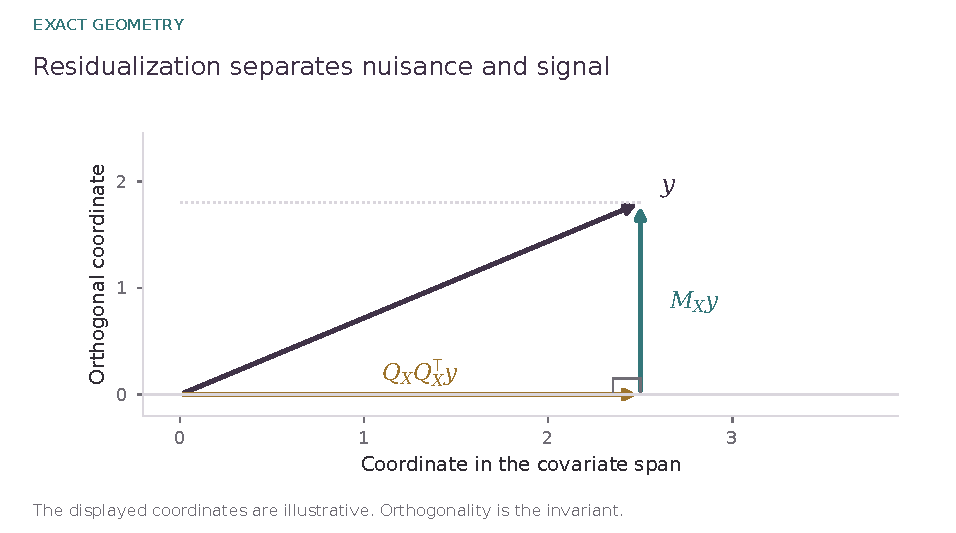
\includegraphics[width=\linewidth]{figures_production/figure_01_residualization_geometry.pdf}
\caption{Orthogonal residualization separates a feature into a component in the covariate span and a component retained by $M_X$. The diagram is an illustrative coordinate model. The identity behind it is the exact projector decomposition.}
\label{fig:residualization-geometry}
\end{figure}


\section{Variant-block Gram decomposition}\label{sec:final-8}

Partition the variant indices into disjoint blocks
\[
\{1,\ldots,m\}
=
J_1\sqcup\cdots\sqcup J_B.
\]
Let
\[
G_b=G_{[:,J_b]},
\qquad
W_b=W_{J_b,J_b},
\qquad
A_b=M_XG_bW_b^{1/2}.
\]
Then
\[
A=[A_1\ \cdots\ A_B].
\]

\begin{theorem}[Additive block Gram identity]\label{claim:final-8-1}
\[
\boxed{
K
=
AA^\top
=
\sum_{b=1}^B A_bA_b^\top
=
M_X
\left(
\sum_{b=1}^B G_bW_bG_b^\top
\right)
M_X.
}
\]
\end{theorem}

\begin{proof}
Horizontal concatenation gives
\[
[A_1\ \cdots\ A_B]
\begin{bmatrix}
A_1^\top\\
\vdots\\
A_B^\top
\end{bmatrix}
=
\sum_bA_bA_b^\top.
\]
The final form follows from
\(A_b=M_XG_bW_b^{1/2}\) and
\(M_X^\top=M_X=M_X^2\).
\end{proof}

\begin{remark}\label{claim:final-8-2}
The theorem is exact for every partition.  Block boundaries are execution
parameters, not statistical parameters.
\end{remark}


\begin{figure}[htbp]
\centering
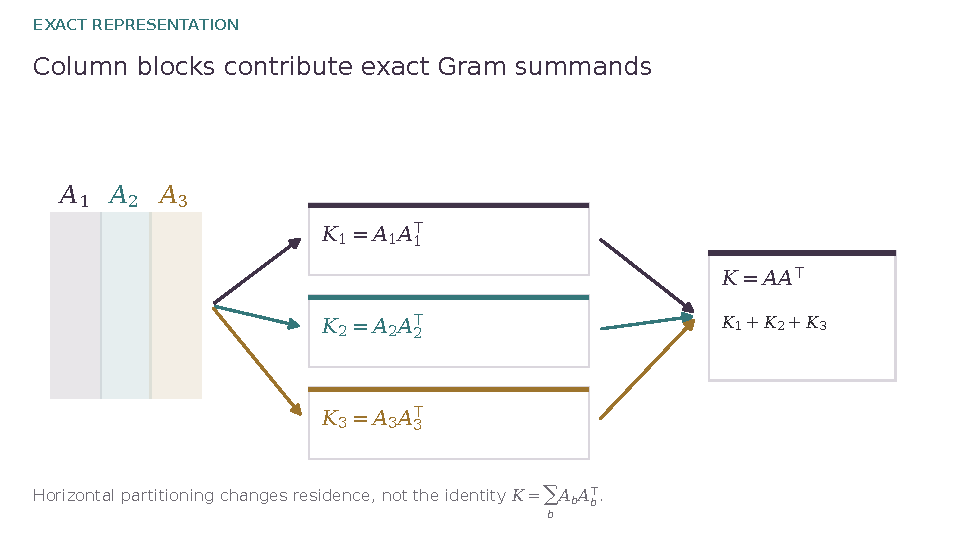
\includegraphics[width=\linewidth]{figures_production/figure_02_exact_block_kernel_assembly.pdf}
\caption{Each resident column block contributes a complete sample-space Gram summand $A_bA_b^{\mathsf T}$. Adding the summands recovers $AA^{\mathsf T}$ exactly. Storage partitioning changes residence and evaluation order, not the represented operator.}
\label{fig:block-kernel-assembly}
\end{figure}


\section{Exact streamed kernel actions}\label{sec:final-9}

\begin{theorem}[One-pass sample-space streaming action]\label{claim:final-9-1}
For every block vector \(V\in\mathbb R^{n\times s}\),
\[
\boxed{
KV
=
M_X
\sum_{b=1}^B
G_bW_bG_b^\top
M_XV.
}
\]
\end{theorem}

\begin{proof}
Apply the additive block Gram identity to \(KV\), then associate each block
product as
\[
G_bW_b(G_b^\top M_XV).
\]
\end{proof}

\begin{algorithm}[Streamed \(KV\)]\label{claim:final-9-2}
\begin{enumerate}[label=\arabic*.]
\item Compute \(U=M_XV\).
\item Set \(Y=0\).
\item For each resident block \(b\), compute
\[
T_b=G_b^\top U,
\qquad
Y\leftarrow Y+G_b(W_bT_b).
\]
\item Return \(M_XY\).
\end{enumerate}
\end{algorithm}

\begin{corollary}[Working memory independent of total variant count]\label{claim:final-9-3}
If at most \(c\) variants are resident and the block-vector width is \(s\),
then the algebraic working set is
\[
\boxed{
O(nc+ns+cs+np),
}
\]
independent of total variant count \(m\).
\end{corollary}


\section{Streamed factor actions and Golub--Kahan}\label{sec:final-10}

Let \(V\in\mathbb R^{m\times s}\) be partitioned conformally:
\[
V=
\begin{bmatrix}
V_1\\
\vdots\\
V_B
\end{bmatrix}.
\]

\begin{theorem}[Streamed \(AV\)]\label{claim:final-10-1}
\[
\boxed{
AV
=
M_X
\sum_{b=1}^B
G_bW_b^{1/2}V_b.
}
\]
\end{theorem}

\begin{theorem}[Streamed \(A^\top U\)]\label{claim:final-10-2}
For \(U\in\mathbb R^{n\times s}\),
\[
\boxed{
(A^\top U)_b
=
W_b^{1/2}G_b^\top M_XU.
}
\]
\end{theorem}

\begin{proof}
Both identities follow by substituting
\(A=M_XGW^{1/2}\) and partitioning the variant coordinate.
\end{proof}

\begin{corollary}[Streaming Golub--Kahan equivalence]\label{claim:final-10-3}
With the same initial state, algorithmic choices, and random draws, any
exact-arithmetic algorithm whose access to \(A\) occurs only through
\(AV\) and \(A^\top U\) produces the same iterates when those products are
implemented by the preceding streamed formulas.
\end{corollary}

This applies directly to block Golub--Kahan bidiagonalization, matrix-free
singular-value iteration, range finding, and restarted variants.  The
factor need not be resident.


\section{Two-pass dual action}\label{sec:final-11}

The variant-space normal operator is
\[
H=A^\top A.
\]

\begin{theorem}[Two-pass streamed dual action]\label{claim:final-11-1}
For every \(V\in\mathbb R^{m\times s}\),
\[
\boxed{
HV=A^\top(AV).
}
\]
The product is evaluated exactly by a streamed pass forming
\(Y=AV\in\mathbb R^{n\times s}\), followed by a second streamed pass
emitting the blocks
\[
(HV)_b=W_b^{1/2}G_b^\top M_XY.
\]
\end{theorem}

This form is particularly natural for variant-space polyphase Krylov
iterations because the right-coordinate blocks can be produced and consumed
sequentially.


\section{Two-dimensional sample/variant tiling}\label{sec:final-12}

A variant block may itself exceed device memory.  Let
\[
H_b=G_bW_b^{1/2}
\]
and partition samples into row tiles \(I_1,\ldots,I_R\).

\begin{theorem}[Two-pass residualized tile construction]\label{claim:final-12-1}
Define
\[
R_b=Q_X^\top H_b.
\]
Then
\[
\boxed{
R_b
=
\sum_r
Q_{X,I_r}^\top H_{b,I_r},
}
\]
and after \(R_b\) is known,
\[
\boxed{
A_{b,I_r}
=
H_{b,I_r}-Q_{X,I_r}R_b.
}
\]
Consequently,
\[
\boxed{
K_{I_r,I_s}
=
\sum_b
A_{b,I_r}A_{b,I_s}^\top.
}
\]
\end{theorem}

\begin{proof}
The first identity is the row-partitioned matrix product
\(Q_X^\top H_b\).  The second is the definition
\(M_XH_b=H_b-Q_XQ_X^\top H_b\).  The last identity is the corresponding
sample-tile expansion of \(AA^\top\).
\end{proof}

With sample tile height \(t\) and resident variant width \(c\), the dominant
working storage, including a resident covariate tile, is
\[
O(tc+pc+tp+t^2).
\]
This count excludes the backing input store, completed output blocks,
allocator overhead, and library workspaces.


\section{Partition refinement and permutation invariance}\label{sec:final-13}

\begin{theorem}[Partition-refinement invariance]\label{claim:final-13-1}
Let \(\mathcal J\) be any partition of the variants and let
\(\mathcal J'\) refine \(\mathcal J\).  Then
\[
\boxed{
\sum_{J\in\mathcal J}A_JA_J^\top
=
\sum_{J'\in\mathcal J'}A_{J'}A_{J'}^\top
=
AA^\top.
}
\]
The analogous streamed operator action is also invariant.
\end{theorem}

\begin{proof}
Each coarse block is a disjoint union of refined blocks.  Apply the additive
Gram theorem within each coarse block and sum.
\end{proof}

\begin{corollary}[Adaptive memory splitting]\label{claim:final-13-2}
A runtime may recursively subdivide any block that exceeds available device
memory without changing the exact operator.
\end{corollary}

\begin{proposition}[Variant permutation invariance]\label{claim:final-13-3}
If the columns of \(G\) and the diagonal entries of \(W\) are permuted by the
same permutation, \(K\) and every streamed sample-space action are unchanged.
\end{proposition}


\begin{figure}[htbp]
\centering
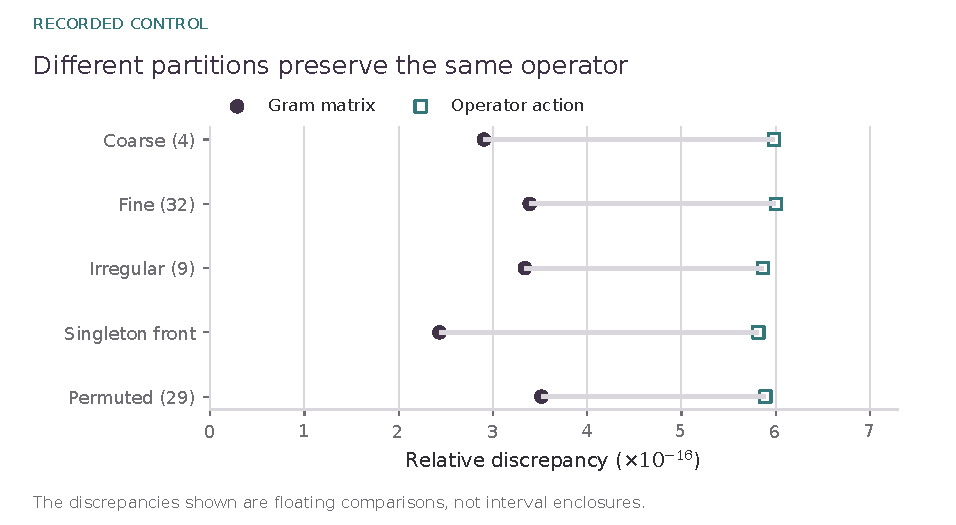
\includegraphics[width=\linewidth]{figures_production/figure_08_partition_invariance.pdf}
\caption{Gram and operator-action discrepancies for five retained partition controls. Horizontal connectors pair the two measurements for each partition. The small floating discrepancies support the implementation check, while the partition identity itself is exact algebra.}
\label{fig:partition-invariance}
\end{figure}


\section{Memory planning law}\label{sec:final-27}

Let \(d\) be the number of bytes per floating scalar, \(c\) the resident
variant count, \(s\) the Krylov width, and \(p\) the covariate rank.
Ignoring library workspace and allocator overhead, a streamed sample-space
action has working memory on the order of
\[
\boxed{
d\,[nc+2ns+cs+np+O(ps+c)].
}
\]

The full factor costs
\[
dnm.
\]

For fixed \(n,p,s,c\),
\[
\boxed{
\frac{M_{\rm stream}}{M_{\rm full}}
=
O\!\left(
\frac{c}{m}
+
\frac{s}{m}
+
\frac{p}{m}
\right),
}
\]
so device memory remains bounded as total variant count grows.

\begin{table}[htbp]
\centering
\caption{Algebraic float64 memory model for \(n=2000\), \(p=4\),
Krylov width \(s=16\), resident variant block \(c=1024\), and
sample tile height \(t=256\).}
\begin{tabular}{rrrr}
\toprule
\(m\) & full factor (MiB) & streamed \(KV\) (MiB) & tiled Gram (MiB)\\
\midrule
10,000 & 152.6 & 16.308 & 8.555\\
50,000 & 762.9 & 16.308 & 8.555\\
100,000 & 1,525.9 & 16.308 & 8.555\\
500,000 & 7,629.4 & 16.308 & 8.555\\
1,000,000 & 15,258.8 & 16.308 & 8.555\\
\bottomrule
\end{tabular}
\end{table}


\begin{figure}[htbp]
\centering
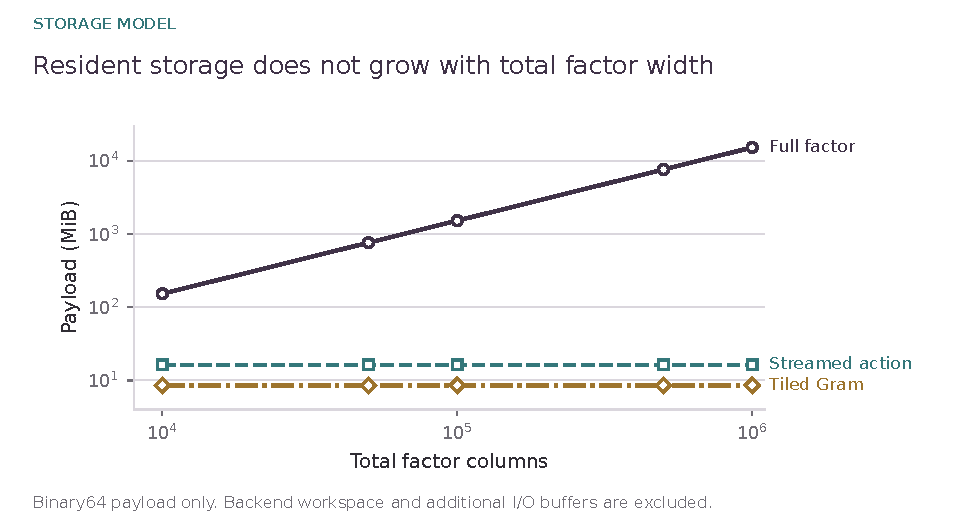
\includegraphics[width=\linewidth]{figures_production/figure_03_memory_law.pdf}
\caption{Binary64 payload as total factor width increases. The complete factor grows with $m$, while the streamed and tiled payloads remain constant at fixed resident dimensions. These are algebraic sizing data, not measurements of total device allocation.}
\label{fig:memory-law}
\end{figure}



\section{The running example in three storage blocks}\label{sec:worked-stream}
Partition the factor of Section~\ref{sec:worked-law} into consecutive pairs of columns,
\[
A=[A_1\ A_2\ A_3],\qquad A_i\in\mathbb R^{4\times2}.
\]
Although $A_2=A_3$, both column groups must be counted. Their Gram contributions are
\[
A_1A_1^\top=\frac12
\begin{pmatrix}1&0&1&0\\0&1&0&1\\1&0&1&0\\0&1&0&1\end{pmatrix},\qquad
A_2A_2^\top=A_3A_3^\top=\frac12
\begin{pmatrix}1&0&-1&0\\0&1&0&-1\\-1&0&1&0\\0&-1&0&1\end{pmatrix}.
\]
The sum is $K$. Merging the last two blocks preserves it. Discarding $A_3$ instead changes the operator and its probability law.

For the declared vector $v=(1,2,-1,0)^\top$, the action can be evaluated without forming any block Gram matrix:
\[
\sum_{j=1}^3 A_j(A_j^\top v)=Kv=(2,3,-2,-1)^\top.
\]
The symbolic check confirms both storage partitions. Every column remains represented. Dropping an operator coupling instead changes the operator and requires the error analysis developed next.

\chapter{Polyphase propagation and scheduling}\label{ch:phases}
\chapterlead{Storage blocks say where data are held. Structural phases say where an
operator can send a vector. Exact zero couplings produce finite propagation
frontiers. Weak couplings produce a controlled leakage problem instead.
The scheduler must distinguish those two cases and state what knowledge of
the phase graph is assumed.}
\section{Polyphase structure}\label{sec:final-14}

Let the phase projectors form an orthogonal decomposition of variant space:
\[
P_h^\top=P_h=P_h^2,\qquad P_hP_g=0\ (h\ne g),\qquad \sum_hP_h=I.
\]
Thus $P_h$ projects onto variant phase $h$. Again set
\[
H=A^\top A.
\]
Define the exact phase graph by
\[
g\to h
\quad\Longleftrightarrow\quad
P_hHP_g\ne0.
\]

\begin{theorem}[Polyphase light cone]\label{claim:final-14-1}
If the graph distance from phase \(g\) to phase \(h\) exceeds \(k\), then
\[
\boxed{
P_hH^kP_g=0.
}
\]
\end{theorem}

\begin{proof}
Insert the projector resolution
\(\sum_jP_j=I\) between successive factors of \(H\).  Every nonzero term in
\(P_hH^kP_g\) corresponds to a phase path of length \(k\).  If no such path
exists, every term vanishes.
\end{proof}


\begin{figure}[htbp]
\centering
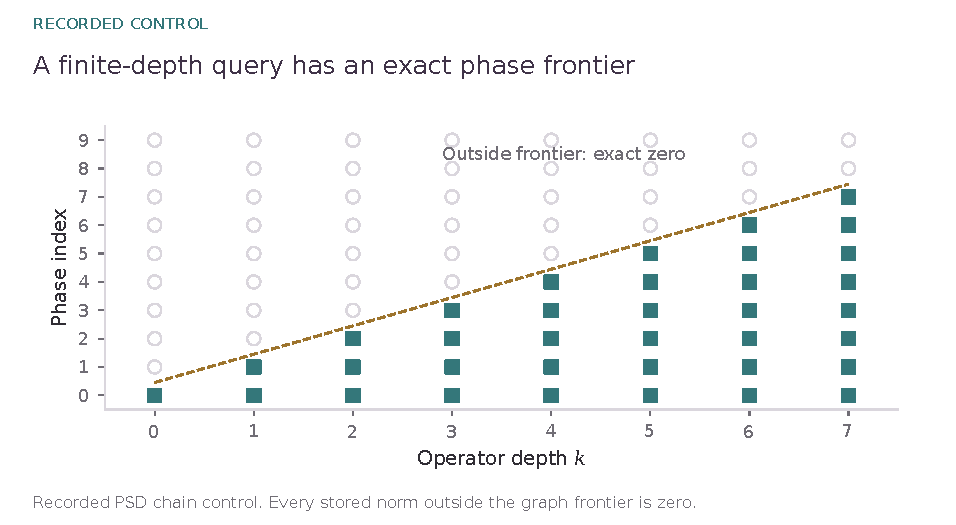
\includegraphics[width=\linewidth]{figures_production/figure_04_polyphase_lightcone.pdf}
\caption{Active phase-depth pairs in the retained PSD chain control are filled squares. Open circles mark inactive pairs. All stored norms beyond the graph frontier are zero. The dashed boundary separates reachable phases from those that the finite-depth query cannot use.}
\label{fig:polyphase-lightcone}
\end{figure}

\begin{theorem}[Streaming-polyphase composition]\label{claim:final-14-2}
At Krylov depth \(k\), an exact matrix-free iteration may omit every phase
outside the exact light cone.  Within each active phase, arbitrary storage
refinement may be used.
\end{theorem}

\begin{proof}
The light-cone theorem removes inactive phase contributions exactly.
Partition-refinement invariance shows that the remaining active phase
operators may be streamed through any exact subpartition.
\end{proof}

This is the key composition law:
\[
\boxed{
\text{mathematical locality}
\longrightarrow
\text{active phases}
\longrightarrow
\text{active storage blocks}.
}
\]


\section{Certified approximate light cones}\label{sec:final-15}
\label{sec:approx-lightcone}

The exact light-cone theorem requires literal zero phase couplings.  Real LD,
annotation, and feature graphs are often only approximately sparse.  This
section replaces exact support by a computable phasewise envelope.

Let the phase projectors be $P_1,\ldots,P_q$, and let $X$ be a vector or block
vector.  Define its phase-norm profile
\[
\rho(X)_g=\lVert P_gX\rVert_F,
\]
and define the nonnegative phase-transfer matrix
\[
\mathcal B_{hg}=\lVert P_hHP_g\rVert_2.
\]
The matrix $\mathcal B$ records the strength of every one-step phase transfer
without assuming that weak couplings vanish.

\begin{theorem}[Weighted phase-transfer envelope]
\label{thm:weighted-transfer}
For every block vector $X$,
\[
\boxed{
\rho(HX)\leq \mathcal B\rho(X)
}
\]
componentwise.  Consequently, for every integer $k\geq0$,
\[
\boxed{
\rho(H^kX)\leq \mathcal B^k\rho(X).
}
\]
\end{theorem}

\begin{proof}
Using $\sum_gP_g=I$ and submultiplicativity,
\[
\begin{aligned}
\lVert P_hHX\rVert_F
&=\left\lVert\sum_gP_hHP_gX\right\rVert_F\\
&\leq\sum_g\lVert P_hHP_g\rVert_2\lVert P_gX\rVert_F\\
&=(\mathcal B\rho(X))_h.
\end{aligned}
\]
Iteration gives the power bound.
\end{proof}

Now choose a symmetric set of retained phase blocks and define
\[
H_0=\sum_{(h,g)\in\mathcal E_0}P_hHP_g.
\]
Let
\[
(\mathcal B_0)_{hg}=
\begin{cases}
\mathcal B_{hg},&(h,g)\in\mathcal E_0,\\
0,&\text{otherwise},
\end{cases}
\qquad
\mathcal R=\mathcal B-\mathcal B_0.
\]
Symmetric pair retention preserves self-adjointness of $H_0$, although the
following error theorem does not require positive semidefiniteness of $H_0$.

\begin{theorem}[Thresholded-power certificate]
\label{thm:thresholded-power}
For every $k\geq1$,
\[
\boxed{
\rho\bigl((H^k-H_0^k)X\bigr)
\leq
(\mathcal B^k-\mathcal B_0^k)\rho(X).
}
\]
In particular,
\[
\boxed{
\lVert(H^k-H_0^k)X\rVert_F
\leq
\left\lVert(\mathcal B^k-\mathcal B_0^k)\rho(X)\right\rVert_2.
}
\]
\end{theorem}

\begin{proof}
Write $E=H-H_0$.  The telescoping identity gives
\[
H^k-H_0^k
=
\sum_{j=0}^{k-1}H^{k-1-j}EH_0^j.
\]
The block-norm matrix of $E$ is $\mathcal R$.  Applying
Theorem~\ref{thm:weighted-transfer} successively to each term gives
\[
\rho\bigl((H^k-H_0^k)X\bigr)
\leq
\sum_{j=0}^{k-1}
\mathcal B^{k-1-j}\mathcal R\mathcal B_0^j\rho(X).
\]
The matrix telescoping identity
\[
\mathcal B^k-\mathcal B_0^k
=
\sum_{j=0}^{k-1}
\mathcal B^{k-1-j}(\mathcal B-\mathcal B_0)\mathcal B_0^j
\]
yields the phasewise formula.  Orthogonality of the phase projectors gives
\[
\lVert Y\rVert_F^2=\sum_h\lVert P_hY\rVert_F^2,
\]
which proves the global bound.
\end{proof}

\begin{corollary}[Certified approximate light cone]
\label{cor:approx-lightcone}
Assume $X$ is supported on a set of start phases $S$.  If phase $h$ is not
reachable from $S$ by a retained path of length at most $k$, then
\[
P_hH_0^kX=0
\]
and
\[
\boxed{
\lVert P_hH^kX\rVert_F
\leq
\bigl[(\mathcal B^k-\mathcal B_0^k)\rho(X)\bigr]_h.
}
\]
Thus an exact zero outside the retained light cone is replaced by a certified
nonzero leakage budget.
\end{corollary}

\begin{corollary}[Scalar threshold law]\label{claim:final-15-4}
For any induced matrix norm, let
\[
M=\max\{\lVert\mathcal B\rVert,\lVert\mathcal B_0\rVert\}.
\]
Then
\[
\boxed{
\lVert\mathcal B^k-\mathcal B_0^k\rVert
\leq
kM^{k-1}\lVert\mathcal R\rVert.
}
\]
Hence weak discarded coupling produces a first-order error bound proportional
to the discarded transfer norm and to the Krylov depth.
\end{corollary}

\begin{theorem}[Krylov-polynomial certificate]
\label{thm:polynomial-certificate}
Let
\[
p(t)=\sum_{j=0}^d a_jt^j.
\]
Then
\[
\boxed{
\rho\bigl((p(H)-p(H_0))X\bigr)
\leq
\sum_{j=1}^d
|a_j|(\mathcal B^j-\mathcal B_0^j)\rho(X).
}
\]
\end{theorem}

\begin{proof}
Apply Theorem~\ref{thm:thresholded-power} to every nonconstant power and use
the triangle inequality.  The constant terms cancel.
\end{proof}

The theorem compares the same polynomial $p$ and the same starting block
$X$ under the two operators. It therefore covers fixed polynomial filters
and fixed linear combinations of Krylov powers, not only $H^kX$.
If an adaptive iteration selects different coefficients or restart vectors
under $H$ and $H_0$, their discrepancy requires a separate bound. The
fixed-polynomial certificate alone does not control that additional change.

\begin{corollary}[Certified phase pruning]\label{claim:final-15-6}
If a thresholded phase graph is chosen so that
\[
\left\lVert
(\mathcal B^k-\mathcal B_0^k)\rho(X)
\right\rVert_2
\leq\tau,
\]
then replacing $H^kX$ by $H_0^kX$ incurs Frobenius error at most $\tau$.
The same statement holds for a Krylov polynomial with the certificate in
Theorem~\ref{thm:polynomial-certificate}.
\end{corollary}

This turns graph thresholding into an error-budget decision.  A phase or
interface is not discarded because it merely appears small. It is discarded
only when the weighted sum of all paths using discarded couplings remains
inside the requested tolerance.

\begin{figure}[htbp]
\centering
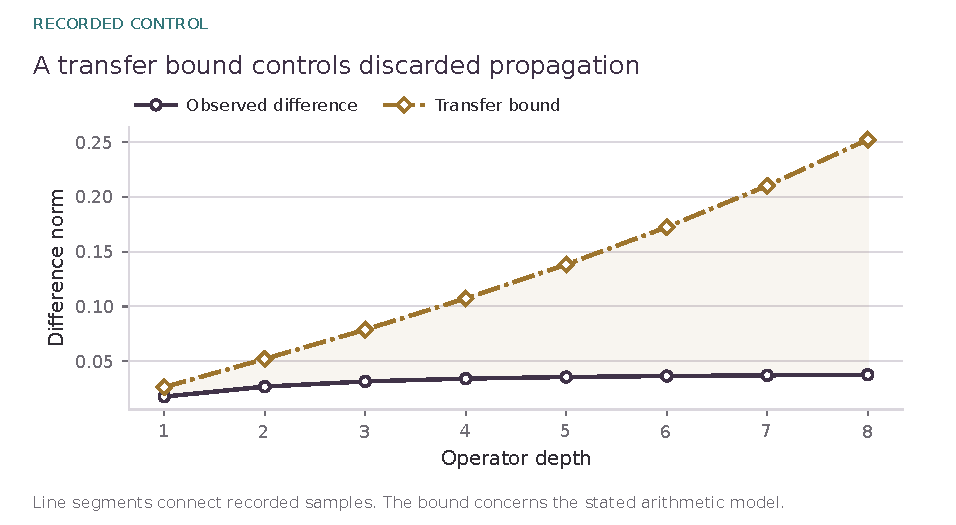
\includegraphics[width=\linewidth]{figures_production/figure_09_approximate_lightcone_certificate.pdf}
\caption{Observed propagation error and the transfer-matrix envelope in the retained PSD control. The envelope remains above the measured error at every tested depth. Shading makes the conservative margin visible without treating it as statistical uncertainty.}
\label{fig:approx-lightcone-certificate}
\end{figure}

\begin{figure}[htbp]
\centering
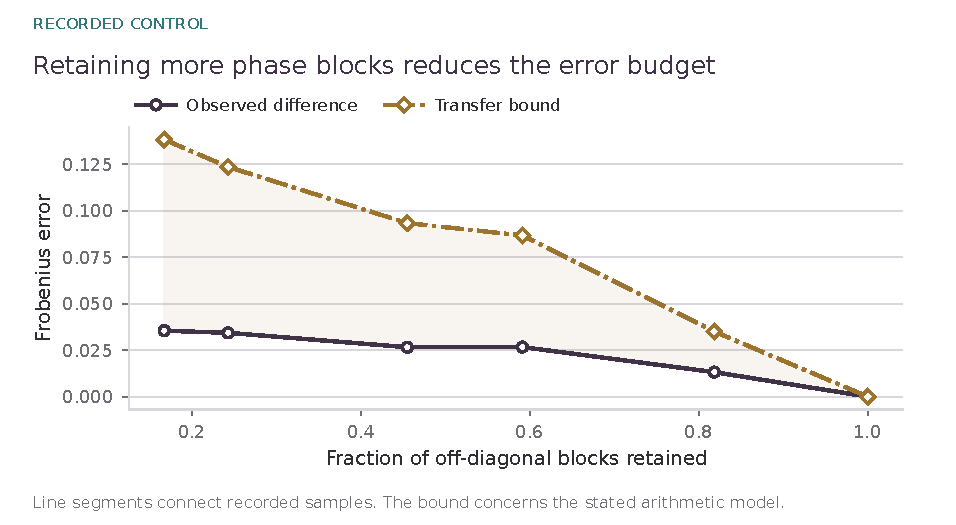
\includegraphics[width=\linewidth]{figures_production/figure_10_threshold_tradeoff.pdf}
\caption{At Krylov depth five, retaining more off-diagonal blocks reduces both the measured truncation error and its transfer bound in this control. Lines join recorded samples. The bound ignores cancellation and singular-vector alignment, so its margin is intentionally conservative.}
\label{fig:threshold-tradeoff}
\end{figure}

\subsection{Numerical audit}

The validation operator has twelve phases of width four.  A block-bidiagonal
factor generates a positive-definite local operator $H_0$, and weak symmetric
long-range blocks are then added to obtain $H$.  Both normalized operators
remain positive definite.  A three-column start block is supported in phase
zero.

For depths one through eight:
\begin{itemize}
\item every observed phase norm lay below $\mathcal B^k\rho(X)$.
\item every observed thresholding error lay below
$(\mathcal B^k-\mathcal B_0^k)\rho(X)$.
\item the largest total observed-error-to-certificate ratio was approximately
$0.669$.
\end{itemize}

A separate hard-threshold sweep retained between $22$ and $132$ directed
off-diagonal phase blocks.  Every measured depth-five error remained below its
certificate. The largest observed-error-to-certificate ratio was approximately
$0.376$.  Finally, a degree-four signed polynomial in $H$ satisfied the
phasewise polynomial certificate in all twelve phases, with maximum ratio
approximately $0.068$.

These computations validate the implementation and illustrate sharpness.  The
universal result is supplied by the preceding proofs, not by the finite test.



\section{Certified budget-optimal phase scheduling}\label{sec:final-16}
\label{sec:budget-scheduler}

The preceding section answers a validation question: given a retained phase
operator $H_0$, how large can the Krylov error be?  This section turns that
certificate into a selection rule.  The goal is to remove as much phase
communication as possible while remaining inside a prescribed error budget.

Let $\mathcal E$ denote the set of undirected off-diagonal phase pairs.  Because
$H$ is self-adjoint, $\mathcal B$ is symmetric.  For a phase pair
$e=\{h,g\}$ define the nonnegative matrix $\Delta_e$ by
\[
(\Delta_e)_{hg}=\mathcal B_{hg},\qquad
(\Delta_e)_{gh}=\mathcal B_{gh},
\]
with every other entry zero.  If $\mathcal O\subseteq\mathcal E$ is the set
of omitted pairs, define
\[
\mathcal B_{\mathcal O}
=\mathcal B-\sum_{e\in\mathcal O}\Delta_e.
\]
The diagonal is always retained. The corresponding pruned operator is
\[
H_{\mathcal O}
=H-\sum_{\{h,g\}\in\mathcal O}
\bigl(P_hHP_g+P_gHP_h\bigr).
\]
Thus $\mathcal B_{\mathcal O}$ is its block-norm transfer matrix.

For depth $k\ge1$ and starting phase profile $\rho_0=\rho(X)$, define the
\emph{edge risk vector}
\[
\boxed{
q_e^{(k)}
=
\sum_{j=0}^{k-1}
\mathcal B^{k-1-j}\Delta_e\mathcal B^j\rho_0
}
\]
and its scalar risk
\[
\boxed{
\beta_e^{(k)}=\lVert q_e^{(k)}\rVert_2.
}
\]
Unlike the raw block norm $\mathcal B_{hg}$, this quantity depends on the
start profile and on Krylov depth.

\begin{theorem}[Edge-additive leakage majorant]
\label{thm:edge-additive-majorant}
For every omitted set $\mathcal O\subseteq\mathcal E$,
\[
\boxed{
0\le
(\mathcal B^k-\mathcal B_{\mathcal O}^k)\rho_0
\le
\sum_{e\in\mathcal O}q_e^{(k)}
}
\]
componentwise.  Consequently,
\[
\boxed{
\lVert(H^k-H_{\mathcal O}^k)X\rVert_F
\le
\left\lVert
(\mathcal B^k-\mathcal B_{\mathcal O}^k)\rho_0
\right\rVert_2
\le
\sum_{e\in\mathcal O}\beta_e^{(k)}.
}
\]
\end{theorem}

\begin{proof}
The first inequality in the second display is
Theorem~\ref{thm:thresholded-power}.  For the transfer matrices, the exact
noncommutative telescoping identity is
\[
\mathcal B^k-\mathcal B_{\mathcal O}^k
=
\sum_{j=0}^{k-1}
\mathcal B^{k-1-j}
(\mathcal B-\mathcal B_{\mathcal O})
\mathcal B_{\mathcal O}^j.
\]
All matrices and $\rho_0$ are nonnegative, and
$0\le\mathcal B_{\mathcal O}\le\mathcal B$ entrywise.  Hence
\[
\mathcal B_{\mathcal O}^j\rho_0
\le
\mathcal B^j\rho_0.
\]
Substituting
\[
\mathcal B-\mathcal B_{\mathcal O}
=
\sum_{e\in\mathcal O}\Delta_e
\]
and distributing the sum gives the componentwise majorant.  The final scalar
bound follows from the Euclidean triangle inequality.
\end{proof}

\begin{corollary}[Polynomial edge-risk certificate]\label{claim:final-16-2}
Let
\[
p(t)=\sum_{d=0}^{D}a_dt^d.
\]
Define
\[
q_e^{(p)}
=
\sum_{d=1}^{D}|a_d|q_e^{(d)},
\qquad
\beta_e^{(p)}=\lVert q_e^{(p)}\rVert_2.
\]
Then
\[
\boxed{
\lVert(p(H)-p(H_{\mathcal O}))X\rVert_F
\le
\sum_{e\in\mathcal O}\beta_e^{(p)}.
}
\]
Thus the same scheduling machinery applies to finite Krylov combinations and
polynomial filters.
\end{corollary}

\begin{corollary}[Query-invisible phase pair]\label{claim:final-16-3}
If
\[
\Delta_e\mathcal B^j\rho_0=0
\qquad
\text{for every }0\le j<k,
\]
then
\[
\beta_e^{(k)}=0.
\]
Therefore a phase pair can be large in operator norm and still have zero
risk for a particular finite-depth query.  A magnitude-only threshold cannot
represent this distinction.
\end{corollary}

\subsection{Equal-cost optimality}

Suppose each retained phase pair has the same communication or scheduling
cost, and fix a budget $\tau\ge0$. Under the additive certificate, a set of
omitted pairs is feasible if
\[
\sum_{e\in\mathcal O}\beta_e^{(k)}\le\tau.
\]
Sort the risks as
\[
\beta_{(1)}\le\beta_{(2)}\le\cdots\le\beta_{(N)}.
\]

\begin{theorem}[Cardinality-optimal certified pruning]
\label{thm:unit-cost-optimal}
Let $r\in\{0,\ldots,N\}$ be the largest integer satisfying
\[
\sum_{i=1}^{r}\beta_{(i)}\le\tau.
\]
Then omitting the $r$ least-risk phase pairs is feasible, and no feasible
omitted set can contain more than $r$ pairs under the scalar additive
certificate.
\end{theorem}

\begin{proof}
If $r=N$, every candidate pair can be omitted and optimality is immediate.
Otherwise, among all subsets of cardinality $r+1$, the smallest possible sum
of risks is
\[
\sum_{i=1}^{r+1}\beta_{(i)}.
\]
By maximality of $r$, that sum exceeds $\tau$.  Hence no set of $r+1$ omitted
pairs is feasible.  The prefix of length $r$ is feasible by construction.
\end{proof}

Optimality is relative to the scalar additive certificate, not to the actual
operator error or to every tighter certificate. The exact transfer envelope
can leave additional slack.

\subsection{Exact-envelope refinement}

After the cardinality-optimal additive schedule is found, recomputing
\[
\left\lVert
(\mathcal B^k-\mathcal B_{\mathcal O}^k)\rho_0
\right\rVert_2
\]
may reveal unused budget.  Additional pairs can then be removed one at a time,
provided the exact transfer envelope remains below $\tau$.

\begin{proposition}[Certified refinement]\label{claim:final-16-5}
Any sequence of additional omissions accepted only when
\[
\left\lVert
(\mathcal B^k-\mathcal B_{\mathcal O}^k)\rho_0
\right\rVert_2\le\tau
\]
remains a valid $\tau$-certificate for the original operator error.
\end{proposition}

The refinement rule used in the reference implementation chooses, among all
currently feasible next omissions, the pair that produces the smallest
increase in the exact transfer envelope.  It is certified but is not claimed
globally optimal.

\subsection{Unequal communication costs}

Let $c_e\ge0$ denote the communication or storage cost saved by omitting pair
$e$.  Under the scalar additive certificate, the exact discrete selection
problem is
\[
\boxed{
\max_{x_e\in\{0,1\}}
\sum_e c_ex_e
\quad\text{subject to}\quad
\sum_e\beta_e^{(k)}x_e\le\tau.
}
\]
This is the $0$--$1$ knapsack problem.  Hence unequal-cost scheduling is
combinatorial in general.  The implementation supplies a safe
cost-to-risk greedy heuristic. Its output remains certified because it never
exceeds the additive risk budget.  A fractional-knapsack relaxation supplies
an upper bound on the maximum possible saved cost.

\begin{figure}[htbp]
\centering
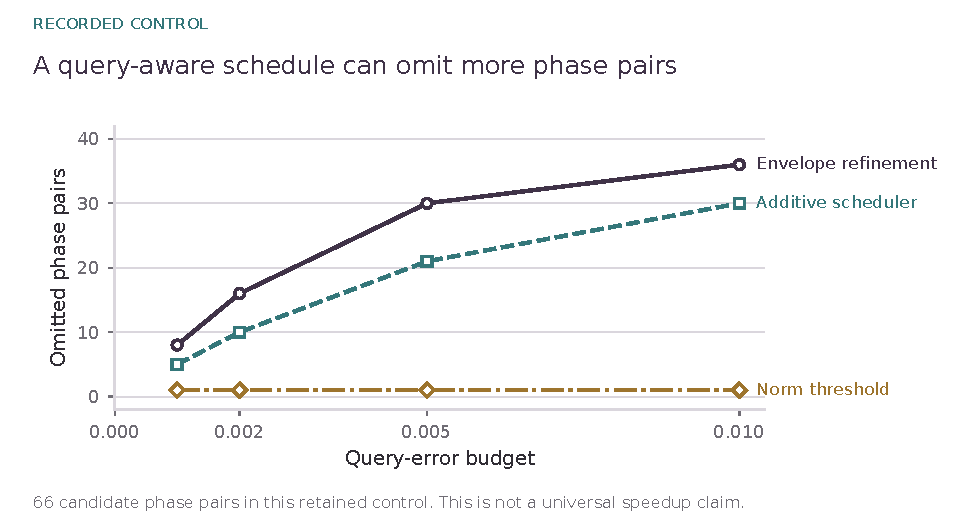
\includegraphics[width=\linewidth]{figures_production/figure_11_budget_scheduler_comparison.pdf}
\caption{Query-aware schedulers omit more phase pairs than a global norm threshold in this depth-five control. Envelope refinement uses slack left by the additive bound. The figure compares retained schedules, not measured execution times or a universal optimality claim.}
\label{fig:budget-scheduler-comparison}
\end{figure}

\begin{figure}[htbp]
\centering
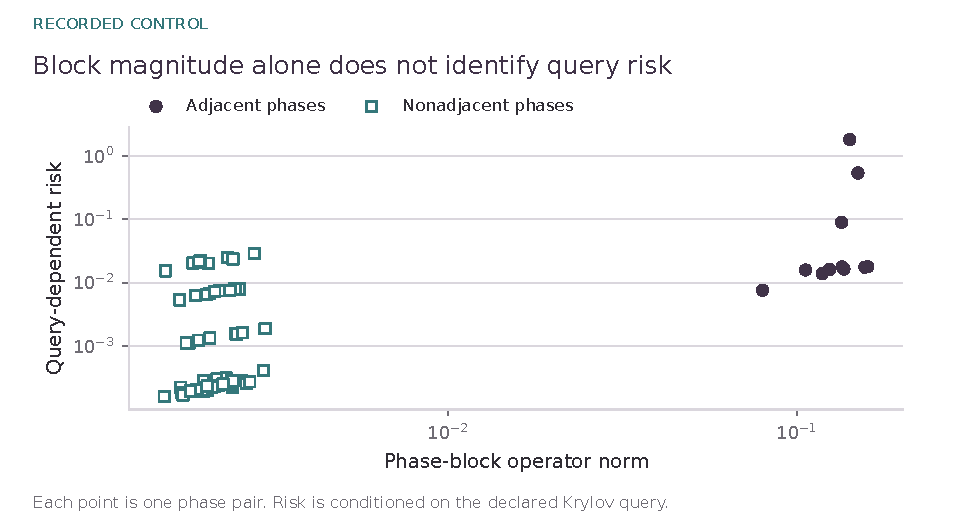
\includegraphics[width=\linewidth]{figures_production/figure_13_edge_risk_vs_block_norm.pdf}
\caption{Block norm and query-dependent risk for each phase pair in the retained control. Adjacency is distinguished by both marker and color. The query risk includes the start profile and finite-depth transfer paths, information absent from the block norm alone.}
\label{fig:edge-risk-vs-norm}
\end{figure}

\subsection{Numerical audit}

The twelve-phase operator from Section~\ref{sec:approx-lightcone} was reused at
Krylov depth five.  There are $66$ undirected off-diagonal phase pairs.
For error budgets $10^{-3}$, $2\times10^{-3}$, $5\times10^{-3}$, and
$10^{-2}$, the additive-optimal scheduler retained respectively
$61$, $56$, $45$, and $36$ pairs.  Exact-envelope refinement reduced those
counts further to
$58$, $50$, $36$, and $30$ pairs while remaining inside budget.

In the same test, the best single global threshold on the raw block norm
retained $65$ pairs at every one of those four budgets.  The difference is
structural: the global threshold is blind to start phase and Krylov depth.

A separate six-phase problem contains $15$ candidate phase pairs, so all
$2^{15}=32768$ subsets can be enumerated.  At four distinct budgets, the
sorted-risk scheduler matched the brute-force cardinality optimum under the
additive certificate in every case.  The exact-envelope greedy refinement also
matched the brute-force exact-envelope optimum in cardinality for all four
budgets in this finite audit.  The latter agreement is empirical and is not
promoted to a theorem.

For an unequal-cost eight-phase test, costs were proportional to the bytes in
symmetric dense phase blocks.  The cost-to-risk heuristic saved $5408$ bytes
out of a $9472$-byte communication proxy while using additive risk $0.011632$
under budget $0.012$.  The fractional relaxation upper bound was $5647.8$
bytes, placing the greedy schedule within about $4.25\%$ of that relaxation
bound on this instance.


\section{Asynchronous double-buffer execution model}\label{sec:final-17}
\label{sec:double-buffer}

The mathematical streaming identities do not require transfers and GEMMs to be
serial.  Consider $B$ storage blocks.  Let $t_b$ be the transfer time for block
$b$ and $c_b$ its device compute time.

\begin{proposition}[Ideal two-buffer pipeline]\label{claim:final-17-1}
In a model with perfect asynchronous overlap, transfer of block $b+1$ may run
while block $b$ is being processed.  The serial one-buffer time is
\[
T_{\rm serial}=\sum_{b=1}^{B}(t_b+c_b),
\]
whereas the two-buffer pipeline time is
\[
\boxed{
T_{\rm pipe}
=
t_1
+
\sum_{b=1}^{B-1}\max\{c_b,t_{b+1}\}
+
c_B.
}
\]
For uniform times $t_b=t$ and $c_b=c$,
\[
T_{\rm pipe}=t+c+(B-1)\max\{t,c\}.
\]
\end{proposition}

\begin{proof}
After the first block arrives, every interior pipeline stage finishes only when
both the current computation and the next transfer have completed.  Their
joint stage duration is therefore the maximum of those two times.  The initial
transfer and final compute cannot be hidden and form the two boundary terms.
\end{proof}

If one resident block uses $M_{\rm block}$ bytes and all other fixed working
state uses $M_{\rm fixed}$ bytes, the corresponding memory models are
\[
M_{\rm single}=M_{\rm fixed}+M_{\rm block},
\qquad
\boxed{
M_{\rm double}=M_{\rm fixed}+2M_{\rm block}.
}
\]
The proposition is a scheduling model, not a hardware timing claim.  PCIe or
NVLink contention, kernel launch overhead, synchronization, page pinning, and
library workspaces can reduce realized overlap.

\begin{figure}[htbp]
\centering
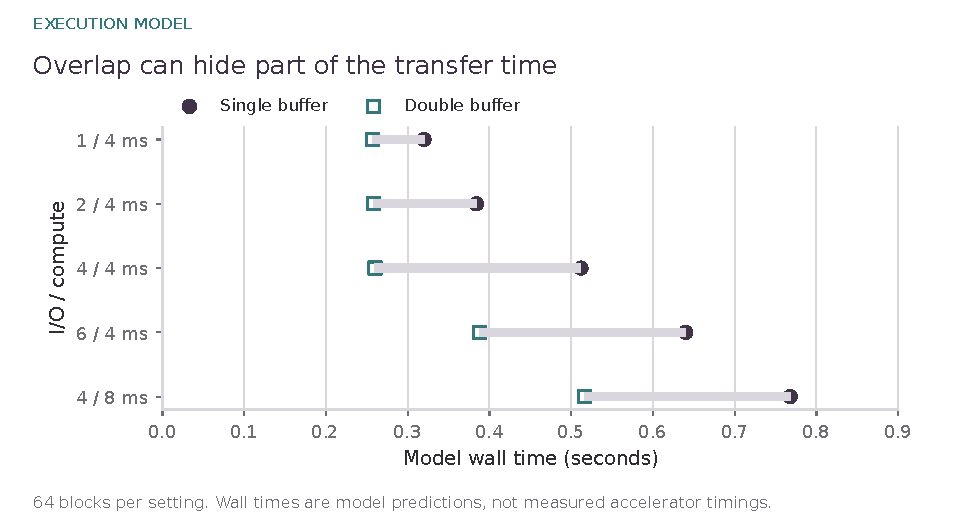
\includegraphics[width=\linewidth]{figures_production/figure_12_double_buffer_model.pdf}
\caption{Modeled wall time for five per-block I/O and compute settings, with 64 blocks in each case. The vertical labels specify I/O time followed by compute time. Connected points compare single and double buffering. These are model predictions, not accelerator measurements.}
\label{fig:double-buffer-model}
\end{figure}



\chapter{Range cores and low-rank interfaces}\label{ch:range}
\chapterlead{After storage and propagation have been organized, the remaining question is
which subspace has actually been resolved. Local ranks govern the width of
phase messages. Orthogonal factor updates carry that information into a small
core with the same nonzero spectrum when the full range has been captured.
An incomplete range requires an additional certificate, developed next.}
\section{Phase-local rank}\label{sec:final-18}

Let \(R\) be a newly generated Krylov residual and
\[
R_h=P_hR.
\]

\begin{theorem}[Minimal exact phase width]\label{claim:final-18-1}
Let
\[
r_h=\operatorname{rank}(R_h).
\]
Every phase-supported basis spanning \(\operatorname{range}(R_h)\) has at
least \(r_h\) vectors, and a rank-revealing QR or compact SVD attains exactly
\(r_h\).
\end{theorem}

This justifies nonuniform Krylov block widths by phase. Here rank means exact
algebraic rank. Discarding a direction by a floating singular-value threshold
is an approximation and requires its own error bound.


\begin{figure}[htbp]
\centering
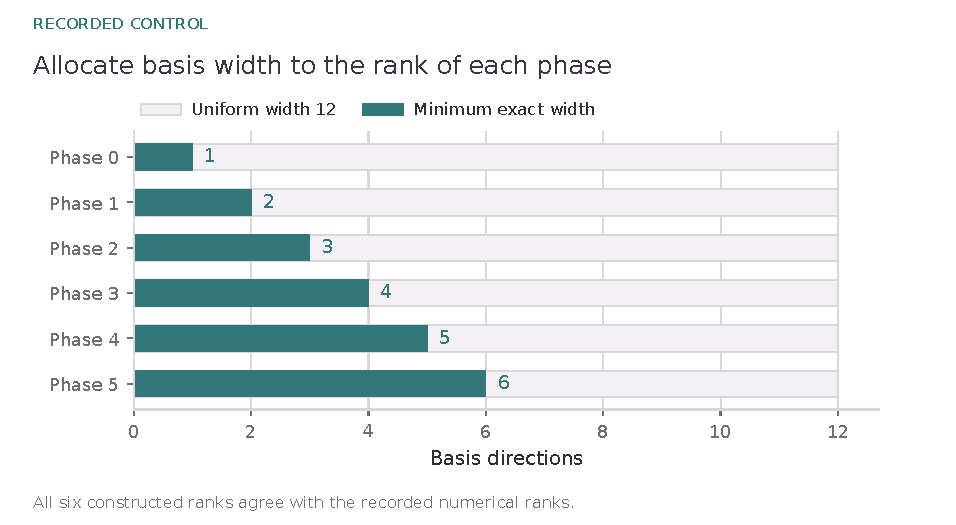
\includegraphics[width=\linewidth]{figures_production/figure_05_phase_local_rank.pdf}
\caption{The recorded six-phase ranks require widths from one through six. Pale bars show the excess capacity of a uniform width of twelve. The comparison uses the rank inventory, not a reconstructed singular-value distribution.}
\label{fig:phase-local-rank}
\end{figure}


\section{Low-rank interface messages}\label{sec:final-19}

If an inter-phase coupling has exact factorization
\[
P_hHP_g
=
U_{hg}V_{hg}^\top
\]
of rank \(r_{hg}\), then
\[
\boxed{
P_hHP_gx
=
U_{hg}(V_{hg}^\top x).
}
\]

This representation reduces storage and communication.  It does not
automatically reduce wall-clock time unless the factors are applied through
batched or fused kernels. A Python reference implementation can lose to
dense BLAS despite lower arithmetic and storage.


\section{Exact QR-core updates}\label{sec:final-20}

Suppose
\[
A=QR,
\qquad
Q^\top Q=I,
\]
and append a new block \(U\).  Set
\[
C=Q^\top U,
\qquad
F=U-QC,
\qquad
F=Q_\perp R_\perp,
\qquad Q_\perp^\top Q_\perp=I,
\qquad Q^\top Q_\perp=0.
\]
Here the columns of \(Q_\perp\) form an orthonormal basis of the nonzero
residual range. Zero residual directions are omitted.

\begin{theorem}[Exact QR-core update]\label{claim:final-20-1}
\[
[A,U]
=
[Q,Q_\perp]
\begin{pmatrix}
R&C\\
0&R_\perp
\end{pmatrix}.
\]
Therefore the nonzero eigenvalues of
\([A,U][A,U]^\top\) are exactly the nonzero eigenvalues of the small
core Gram, with multiplicity. If $\operatorname{range}(Q)=\operatorname{range}(A)$,
the compact residual update also spans exactly $\operatorname{range}([A,U])$.
In that case the core has full row rank and its Gram matrix has no additional
zero eigenvalues.
\end{theorem}

\begin{proof}
The first block product is \(QR=A\). The second is
\(QC+Q_\perp R_\perp=QC+F=U\).  The stated orthogonality
conditions make \([Q,Q_\perp]\) an isometry on the compact core
space.  Left multiplication by this isometry preserves all nonzero singular
values of the core, and squaring them yields the nonzero Gram eigenvalues.
If $Q$ spans exactly the old range and $Q_\perp$ spans exactly the residual
range, their combined range is precisely that of the appended factor.
The core then has full row rank. Without this exact-range hypothesis, unused
basis directions can introduce zero eigenvalues into the core Gram.
\end{proof}

This is useful for overlapping genomic windows and small incremental variant
updates.


\begin{figure}[htbp]
\centering
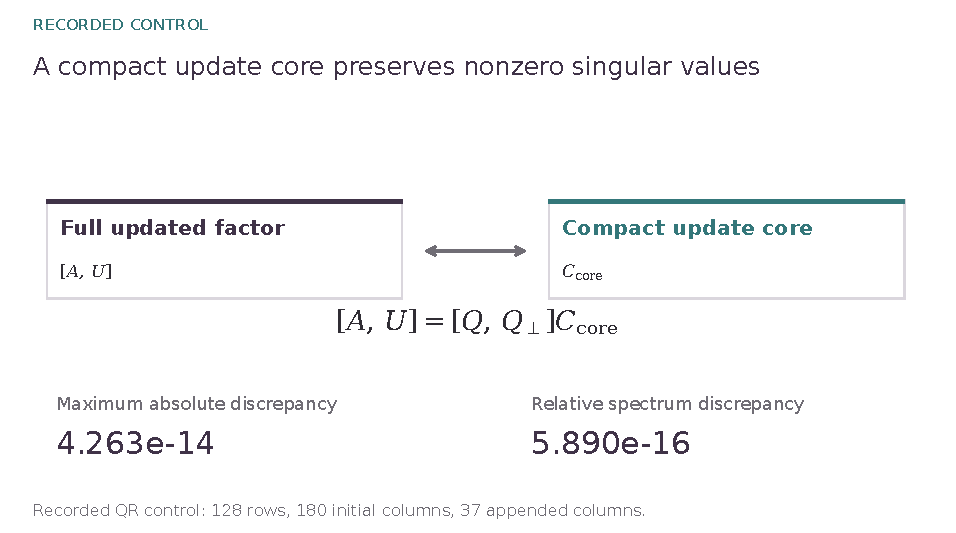
\includegraphics[width=\linewidth]{figures_production/figure_06_qr_core_equivalence.pdf}
\caption{Under the stated orthonormality hypotheses, the full updated factor and its compact core have the same nonzero singular values. The two scalar discrepancies come from the retained 128-row control with 180 initial and 37 appended columns. They are numerical checks of the identity, not a new benchmark.}
\label{fig:qr-core-equivalence}
\end{figure}


\section{Range-core spectral compression}\label{sec:final-21}

Suppose an orthonormal basis \(Q_r\) captures the factor range:
\[
\operatorname{range}(A)\subseteq\operatorname{range}(Q_r).
\]
Then
\[
A=Q_rB,
\qquad
B=Q_r^\top A.
\]

\begin{theorem}[Exact range core]\label{claim:final-21-1}
The nonzero eigenvalues of
\[
K=AA^\top
\]
are exactly the nonzero eigenvalues of
\[
BB^\top,
\]
with multiplicity. If $\operatorname{range}(Q_r)=\operatorname{range}(A)$,
then $BB^\top$ is positive definite on the core space and its entire spectrum
is the nonzero spectrum of $K$.
\end{theorem}

\begin{proof}
Since $A=Q_rB$ and $Q_r^\top Q_r=I$, one has
$AA^\top=Q_r(BB^\top)Q_r^\top$. The map $x\mapsto Q_rx$ is an isometry
from the core space onto $\operatorname{range}(Q_r)$. On that range the two
operators are conjugate, and $AA^\top$ vanishes on its orthogonal complement.
Hence their nonzero eigenvalues agree with multiplicity. If the captured
range equals $\operatorname{range}(A)$, then $B$ has full row rank, so
$BB^\top$ is positive definite. Without that equality, the core may retain
additional zero eigenvalues.
\end{proof}


Thus the computational pipeline can terminate its data-streaming stage after
the range is captured:
\[
\boxed{
\text{streamed data}
\to
\text{small spectral core}
\to
\text{tail evaluation}.
}
\]



\clearpage
\section{An exact core calculation}
Consider the orthonormal range basis and core factor
\[
U=\begin{pmatrix}1&0\\0&1/\sqrt2\\0&1/\sqrt2\end{pmatrix},
\qquad
B=\begin{pmatrix}1&0&1\\0&2&0\end{pmatrix},
\qquad A=UB.
\]
Direct multiplication gives
\[
BB^\top=\begin{pmatrix}2&0\\0&4\end{pmatrix},
\qquad
AA^\top=\begin{pmatrix}2&0&0\\0&2&2\\0&2&2\end{pmatrix}.
\]
The large operator has eigenvalues $4,2,0$. Its two-dimensional core has
exactly the nonzero eigenvalues $4,2$. The Gaussian quadratic form therefore
has the law $4Z_1^2+2Z_2^2$, whether it is computed from the full factor, the
full Gram matrix, or the core.

\subsection*{Why the nonzero-spectrum qualification matters}
Take instead
\[
A=\begin{pmatrix}1&0\\0&0\end{pmatrix},\qquad Q_r=I_2,\qquad B=Q_r^\top A=A.
\]
The captured subspace contains the range of $A$, but is larger than that range.
Both Gram matrices have spectrum $\{1,0\}$. Their nonzero spectrum is
$\{1\}$. Thus the nonzero spectrum of $AA^\top$ cannot be identified with the
\emph{entire} spectrum of $BB^\top$. Choosing the compact basis
$Q_r=(1,0)^\top$ instead gives $B=(1,0)$ and the one-dimensional core Gram
$(1)$. The extra zero records an unused basis direction, not an additional
random contribution. This is why range containment and exact-range equality
have different conclusions in Theorem~\ref{claim:final-21-1}.

The first example in this section has active rank two. It separates algebraic
exactness from backend coverage. The spectral reduction and analytic packet theory remain
valid, but the implemented directed positive-tail backend described in
Chapter~\ref{ch:intervals} requires active rank greater than two. Capturing a
range exactly does not remove a later numerical method's hypotheses.

\chapter{Spectral uncertainty and exact completion}\label{ch:spectrum}
\chapterlead{A useful operator approximation is not automatically a useful tail
approximation. This chapter transports phase-pruning error to eigenvalue
intervals, measures unresolved range through trace information, and completes
small residual ranges exactly. A separate post-verification theorem connects
stored binary64 factors to rigorous spectral intervals.}
\section{From phase pruning to certified quadratic-form tails}\label{sec:final-22}

The previous sections certify the effect of phase pruning on Krylov
propagation.  A SKAT-like test ultimately depends on the spectrum itself, so
one more bridge is needed:
\[
\text{phase pruning}
\longrightarrow
\text{operator error}
\longrightarrow
\text{spectral error}
\longrightarrow
\text{tail-probability error}.
\]

\subsection{Block-norm operator domination}

Let
\[
E=H-H_0
\]
be the self-adjoint error introduced by phase pruning.  Using the same
orthogonal phase projectors \(P_h\), define
\[
\mathcal C_{hg}
=
\|P_hEP_g\|_2.
\]

\begin{theorem}[Block-norm operator certificate]\label{claim:final-22-1}
\[
\boxed{
\|E\|_2
\le
\|\mathcal C\|_2.
}
\]
\end{theorem}

\begin{proof}
For any vector \(x\), let
\[
r_g=\|P_gx\|_2.
\]
Then
\[
\|P_hEx\|_2
\le
\sum_g
\|P_hEP_g\|_2\,\|P_gx\|_2
=
(\mathcal C r)_h.
\]
Orthogonality of the phase decomposition gives
\[
\|Ex\|_2^2
=
\sum_h\|P_hEx\|_2^2
\le
\|\mathcal C r\|_2^2
\le
\|\mathcal C\|_2^2\|r\|_2^2
=
\|\mathcal C\|_2^2\|x\|_2^2.
\]
Taking the supremum over unit vectors proves the claim.
\end{proof}

The important computational point is that \(\mathcal C\) is only a
phase-by-phase matrix.  The same block norms already used to construct the
polyphase scheduler therefore provide a global operator certificate.

\subsection{Weyl enclosure of the quadratic-form coefficients}

Assume
\[
H\succeq0
\]
and let the eigenvalues of \(H\) and \(H_0\), in decreasing order, be
\[
\lambda_i
\qquad\text{and}\qquad
\mu_i.
\]
If
\[
\|H-H_0\|_2\le\varepsilon,
\]
Weyl's inequality gives
\[
|\lambda_i-\mu_i|\le\varepsilon.
\]

\begin{corollary}[Positive spectral interval]\label{claim:final-22-2}
For every \(i\),
\[
\boxed{
\ell_i
=
\max\{0,\mu_i-\varepsilon\}
\le
\lambda_i
\le
u_i
=
\max\{0,\mu_i+\varepsilon\}.
}
\]
\end{corollary}

This remains valid even if symmetric phase pruning makes \(H_0\) slightly
indefinite.

\subsection{Certified generalized-\texorpdfstring{\(\chi^2\)}{chi-square} tail bracket}

For independent standard normal variables \(Z_i\), define
\[
Q_-=\sum_i\ell_iZ_i^2,
\qquad
Q=\sum_i\lambda_iZ_i^2,
\qquad
Q_+=\sum_i u_iZ_i^2.
\]

\begin{theorem}[Stochastic tail enclosure]\label{claim:final-22-3}
For every threshold \(q\),
\[
\boxed{
\Pr(Q_-\ge q)
\le
\Pr(Q\ge q)
\le
\Pr(Q_+\ge q).
}
\]
\end{theorem}

\begin{proof}
Couple all three quadratic forms using the same normal variables \(Z_i\).
Since
\[
0\le\ell_i\le\lambda_i\le u_i
\]
for every \(i\),
\[
Q_-\le Q\le Q_+
\]
almost surely.  Taking upper-tail events yields the result.
\end{proof}

The endpoint probabilities are separate tail queries. Each must satisfy the
hypotheses of the numerical backend used to evaluate it. In particular, zero
lower coefficients can reduce the active rank below the directed backend's
coverage. The stochastic enclosure remains valid in that case, but it does
not by itself supply a supported numerical evaluation. Numerical error is
separate from the spectral uncertainty above.

\subsection{A dual-budget pruning rule}

The local Krylov certificate from the previous section and the global spectral
certificate answer different questions.  The former asks whether omitted
couplings matter to the current Krylov query. The latter asks whether they can
move the spectrum enough to matter to the final test.

An execution schedule should therefore enforce
\[
\boxed{
\sum_{e\in\mathcal O}\beta_e^{(k)}
\le
\tau_K,
\qquad
\|\mathcal C_{\mathcal O}\|_2
\le
\tau_\lambda.
}
\]

The implementation uses a conservative greedy rule: phase pairs are considered
in increasing query-risk order, and a pair is omitted only when adding it
preserves both inequalities.  The rule is certified but is not claimed to be
globally optimal under the two simultaneous constraints.

\begin{figure}[htbp]
\centering
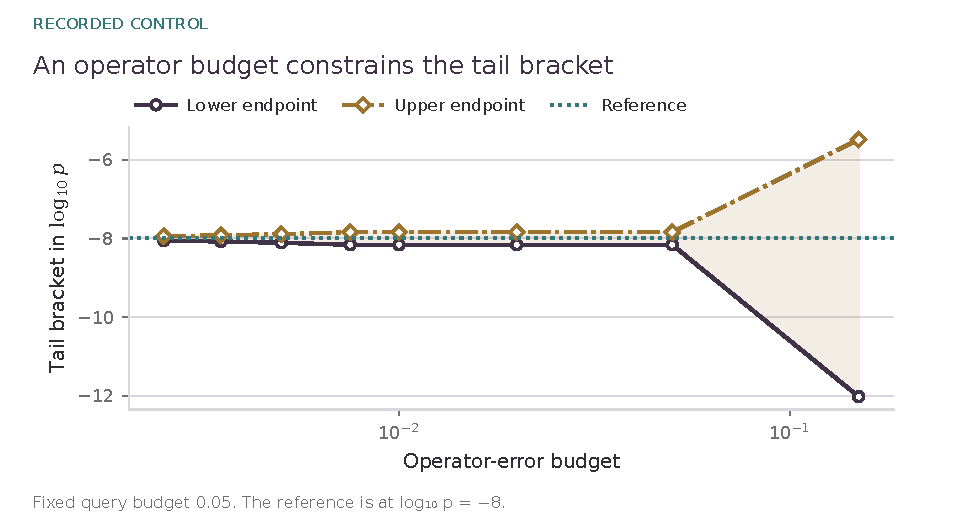
\includegraphics[width=\linewidth]{figures_production/figure_14_dual_budget_tail_bridge.pdf}
\caption{Tail brackets under a fixed query budget and varying operator budgets. The dotted reference is at $\log_{10}p=-8$. A sufficiently loose operator budget admits a strong coupling and widens the bracket even though the query-local constraint still passes.}
\label{fig:dual-budget-tail}
\end{figure}

In the deterministic ten-phase experiment, fixing the query budget at
\(0.05\) and the operator budget at \(0.005\) removed \(23\) of \(45\)
undirected phase pairs.  At a reference probability near \(10^{-8}\), the analytic
tail bracket was
\[
10^{-8.11143}
\le
p
\le
10^{-7.89036},
\]
a width of about \(0.221\) decades. These endpoints summarize the
real-arithmetic error analysis evaluated in floating point, not a directed
rounding enclosure. With an operator budget of \(0.0075\),
\(34\) pairs were removed and the interval widened to about \(0.320\)
decades.  By contrast, allowing a strong coupling to be removed under a very
loose operator budget produced a multi-decade interval.

\subsection{Certify after prune}

There is a second route that does not use the pruned operator as the final
spectral approximation.  Let \(U\) be any orthonormal sample-space basis,
possibly generated cheaply from a pruned or approximate Krylov process, and
define
\[
B=U^\top A,
\qquad
F=(I-UU^\top)A,
\qquad
\delta=\|F\|_2.
\]

\begin{theorem}[Range-core singular-value certificate]\label{claim:final-22-4}
For $A\in\mathbb R^{n\times m}$, list the singular values of $A$ and
$B$ in decreasing order and pad both lists with zeros to length $n$.
Write these lists as $\sigma_i(A)$ and $\widetilde\sigma_i(B)$,
respectively. They are the square roots of the $n$ eigenvalues of
$AA^\top$ and $(UB)(UB)^\top$. Then, for $1\le i\le n$,
\[
\boxed{
\left|
\sigma_i(A)
-
\widetilde\sigma_i(B)
\right|
\le
\delta.
}
\]
Consequently,
\[
\max\{0,\widetilde\sigma_i(B)-\delta\}^2
\le
\lambda_i(AA^\top)
\le
\left(
\widetilde\sigma_i(B)+\delta
\right)^2.
\]
\end{theorem}

\begin{proof}
Because \(U\) has orthonormal columns,
\[
A=UB+F
\]
and
\[
\|A-UB\|_2=\|F\|_2=\delta.
\]
The nonzero singular values of $UB$ and $B$ agree, with multiplicity,
and their zero-padded lists agree in the stated ambient convention.
The standard singular-value perturbation inequality gives the stated bound.
Squaring the nonnegative endpoints gives the eigenvalue interval.
\end{proof}

This provides a useful architecture:
\[
\boxed{
\begin{gathered}
\text{pruned operator for basis discovery}\\
\longrightarrow\ \text{exact streamed factor check}\\
\longrightarrow\ \text{certified spectral core}
\end{gathered}
}
\]

\subsection{A retained negative result}

The preceding theorem is exact, but a correct interval need not be useful.

In a full-rank \(50\times50\) stress test, a pruned Krylov basis of dimensions
\(12\) through \(48\) left range residuals between roughly \(0.87\) and
\(0.99\) times the leading singular value.  The corresponding \(10^{-8}\)
tail intervals were therefore vacuous or thousands of decades wide.  At
dimension \(50\), the range residual fell to approximately
\(1.2\times10^{-15}\), and the tail interval collapsed to the exact value.

\begin{figure}[htbp]
\centering
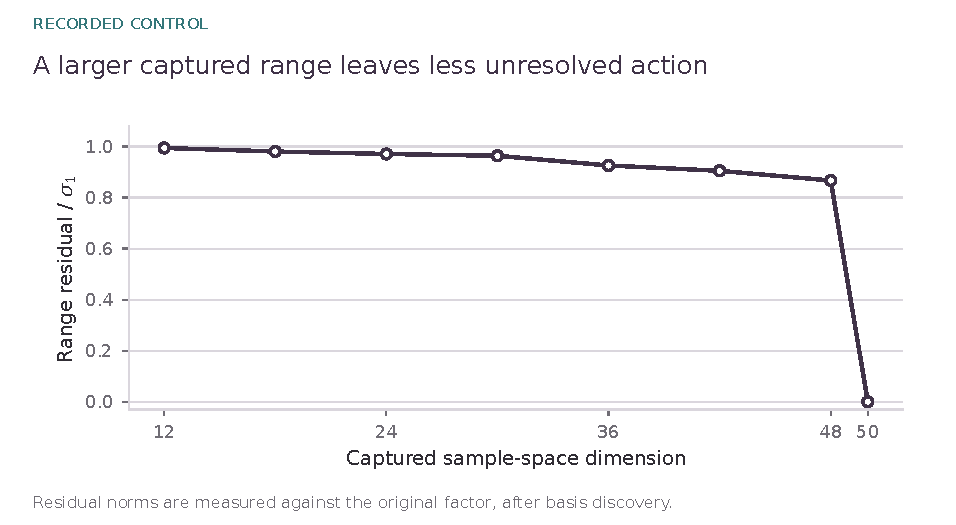
\includegraphics[width=\linewidth]{figures_production/figure_15_range_core_certification.pdf}
\caption{Range residual measured against the original factor after basis discovery. Increasing captured dimension reduces unresolved action in this control, but a useful deep-tail bracket still requires a sufficiently small residual. Basis discovery and certification remain separate steps.}
\label{fig:range-core-cert}
\end{figure}

The practical lesson is that range-core certification is a stopping test, not
a promise that a severely incomplete basis automatically yields a useful
full-spectrum tail bound.



\section{Trace-aware residual certification and exact completion}\label{sec:final-23}

The spectral bridge in the preceding section used an operator-norm residual as
if every unresolved coefficient could move independently by the same amount.
That is rigorous but unnecessarily pessimistic once a nontrivial range basis
has already been captured.  The residual has considerably more structure.

Let \(U\in\mathbb R^{n\times r}\) have orthonormal columns and define
\[
B=U^\top A,
\qquad
F=(I-UU^\top)A.
\]
Then
\[
A=UB+F,
\qquad
U^\top F=0.
\]

\begin{theorem}[Exact core--residual decomposition]\label{claim:final-23-1}
\[
\boxed{
A^\top A
=
B^\top B+F^\top F.
}
\]
In particular the unresolved spectral term
\[
R=F^\top F
\]
is positive semidefinite.
\end{theorem}

\begin{proof}
Expand \((UB+F)^\top(UB+F)\).  The two cross terms vanish because
\(U^\top F=0\), while \(U^\top U=I\).
\end{proof}

This changes the certification problem.  Instead of an arbitrary Hermitian
error, the missing term is a positive residual with measurable spectral
moments.  Define
\[
t=\operatorname{tr}R,
\qquad
v=\operatorname{tr}(R^2),
\qquad
\rho=\|R\|_2.
\]
Then
\[
\boxed{
 t=\|F\|_F^2,
 \qquad
 v=\|FF^\top\|_F^2,
 \qquad
 \rho=\|F\|_2^2.
}
\]
The first quantity is the exact missing mean of the Gaussian quadratic form.
The second records how concentrated the residual spectrum is. The third is
its largest coefficient.

\subsection{A trace--Frobenius--cap MGF envelope}

Set
\[
C=B^\top B,
\qquad
H=C+R,
\qquad
c=\lambda_{\max}(C).
\]
For \(0<2\theta(c+\rho)<1\), put
\[
\alpha=(1-2\theta c)^{-1}.
\]

\begin{theorem}[Trace--Frobenius--cap log-MGF certificate]\label{claim:final-23-2}
For the Gaussian quadratic form with coefficient matrix \(H\),
\[
\kappa_H(\theta)
=-\frac12\log\det(I-2\theta H)
\]
satisfies
\[
\boxed{
\kappa_H(\theta)
\le
\kappa_C(\theta)
+
\theta\alpha t
+
\frac{\theta^2\alpha^2v}
     {1-2\theta\alpha\rho}.
}
\]
\end{theorem}

\begin{proof}
Factor the determinant through the known core:
\[
I-2\theta(C+R)
=
(I-2\theta C)^{1/2}
(I-2\theta T)
(I-2\theta C)^{1/2},
\]
where
\[
T=(I-2\theta C)^{-1/2}
R
(I-2\theta C)^{-1/2}.
\]
Since
\[
\|(I-2\theta C)^{-1/2}\|_2^2=\alpha,
\]
we have
\[
\operatorname{tr}T\le\alpha t,
\qquad
\operatorname{tr}(T^2)\le\alpha^2v,
\qquad
\|T\|_2\le\alpha\rho.
\]
For every eigenvalue \(x\) of \(T\),
\[
-\frac12\log(1-2\theta x)
\le
\theta x
+
\frac{\theta^2x^2}
     {1-2\theta\alpha\rho}.
\]
The scalar inequality follows from the power series of \(-\log(1-u)\) and a
geometric bound on all terms of degree at least two.  Summing over the
eigenvalues of \(T\) proves the result.
\end{proof}

\begin{corollary}[Trace-aware Chernoff upper tail]\label{claim:final-23-3}
For \(Q=Z^\top HZ\) with \(Z\sim N(0,I)\),
\[
\boxed{
\Pr(Q\ge q)
\le
\inf_{0<2\theta(c+\rho)<1}
\exp\{\widehat\kappa_H(\theta)-\theta q\},
}
\]
where \(\widehat\kappa_H\) is the preceding MGF upper bound.
\end{corollary}

A complementary lower endpoint is immediate from
\[
H=C+R\succeq C.
\]
Using the same normal vector,
\[
Z^\top HZ\ge Z^\top CZ
\]
almost surely, and therefore
\[
\boxed{
\Pr(Z^\top CZ\ge q)
\le
\Pr(Z^\top HZ\ge q).
}
\]
The lower endpoint can be evaluated by K-COS on the captured core spectrum,
while the upper endpoint is obtained from the optimized trace-aware Chernoff
bound.

\subsection{Finite stress test}

The previous coefficient-wise Weyl interval was intentionally conservative.
On the same full-rank, 50-dimensional stress test used in the preceding
section, its \(10^{-8}\) tail interval remained thousands of decades wide
until essentially the complete range had been captured.  Preserving the exact
residual trace and higher residual moments changes that behavior substantially.

\begin{table}[htbp]
\centering
\caption{Tail-bracket width in decades at a reference probability near \(10^{-8}\).
The trace/moment bound is conservative but substantially narrower than
coefficient-wise Weyl inflation before full range capture.}
\begin{tabular}{rrrr}
\toprule
Krylov depth & basis dimension & Weyl width & moment width\\
\midrule
4 & 24 & 90,097 & 11.86\\
5 & 30 & 16,511 & 9.76\\
6 & 36 & 3,747 & 7.67\\
7 & 42 & 2,275 & 5.70\\
8 & 48 & 1,165 & 3.39\\
\bottomrule
\end{tabular}
\end{table}

\begin{figure}[htbp]
\centering
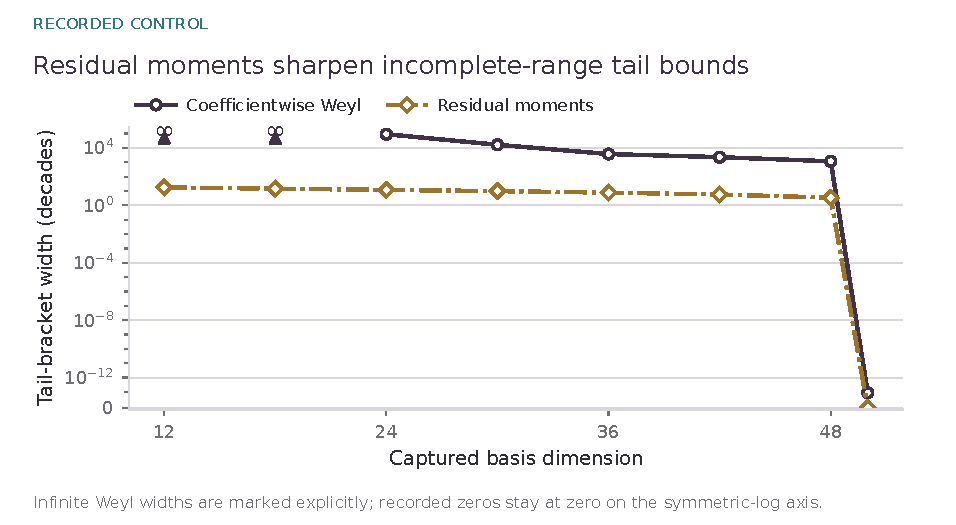
\includegraphics[width=\linewidth]{figures_production/figure_16_trace_moment_vs_weyl.pdf}
\caption{Range-dependent tail-bracket widths. The symmetric-log scale retains the recorded zero at full range capture. Residual moments preserve the amount and concentration of unresolved spectral mass, instead of assigning every coefficient the same worst-case radius. The first two Weyl widths are infinite and are explicitly marked by arrows rather than plotted as finite data.}
\label{fig:trace-moment-vs-weyl}
\end{figure}

A separate random implementation audit used 120 random factor/range pairs and
four admissible positive tilts per pair, for 480 MGF comparisons.  Both the
trace/cap and trace--Frobenius--cap envelopes dominated the exact log MGF in
every tested case.  The trace--Frobenius--cap form was at least as tight as the
trace/cap form in approximately 83.5\% of those comparisons.  This finite
sweep audits the implementation. The theorem above supplies the universal
argument.

\subsection{Residual rank from moments}

The same invariants determine when it is better to stop approximating the
missing spectrum and complete it exactly.  Let
\[
s=\operatorname{rank}F=\operatorname{rank}R.
\]
If the nonzero eigenvalues of \(R\) are \(r_1,\ldots,r_s\), then
\[
t=\sum_i r_i,
\qquad
v=\sum_i r_i^2,
\qquad
r_i\le\rho.
\]

\begin{theorem}[Residual-rank bracket]\label{claim:final-23-4}
\[
\boxed{
\left\lceil
\max\left\{
\frac{t}{\rho},
\frac{t^2}{v}
\right\}
\right\rceil
\le
\operatorname{rank}F
\le
n-r.
}
\]
The zero-residual case is interpreted separately as rank zero.
\end{theorem}

\begin{proof}
The inequality \(t\le s\rho\) gives \(s\ge t/\rho\).  Cauchy--Schwarz gives
\[
t^2
=
\left(\sum_{i=1}^s r_i\right)^2
\le
s\sum_{i=1}^s r_i^2
=sv,
\]
so \(s\ge t^2/v\).  Finally, every column of \(F\) lies in
\(\operatorname{range}(U)^\perp\), whose dimension is \(n-r\).
\end{proof}

Whenever the integer lower bound equals \(n-r\), the missing rank is certified
exactly without computing a residual SVD.

\begin{figure}[htbp]
\centering
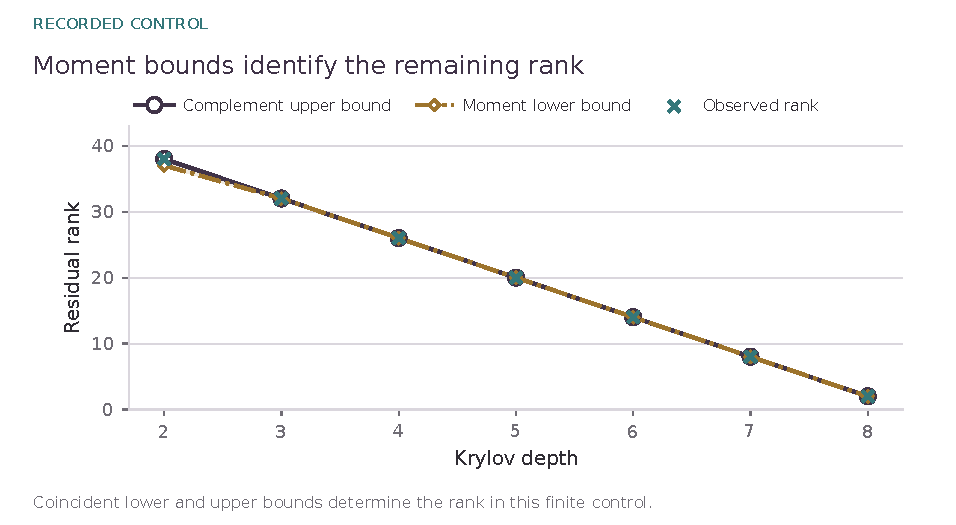
\includegraphics[width=\linewidth]{figures_production/figure_17_residual_rank_completion.pdf}
\caption{Moment lower bounds, complement upper bounds, and observed residual rank in the full-rank control. From depth three onward the bounds coincide. At depth eight only two residual directions remain, permitting a small exact completion.}
\label{fig:residual-rank-completion}
\end{figure}

\subsection{Exact residual completion}

Suppose a compact factorization of the residual is
\[
F=WD,
\]
where the columns of $W$ form an orthonormal basis of
$\operatorname{range}(F)$. Zero residual directions are omitted.
Since this range lies in the orthogonal complement of $U$,
\[
U^\top W=0.
\]

\begin{theorem}[Exact residual completion]\label{claim:final-23-5}
\[
\boxed{
A
=
[U\;W]
\begin{bmatrix}
B\\D
\end{bmatrix}.
}
\]
Consequently, the nonzero singular values of $A$ are exactly the nonzero
singular values, with multiplicity, of the stacked completion core
\[
\mathcal C_{\rm complete}
=
\begin{bmatrix}
B\\D
\end{bmatrix}.
\]
\end{theorem}

\begin{proof}
The decomposition $A=UB+F$ and the identity $F=WD$ give the factorization.
The matrix $[U\;W]$ has orthonormal columns, so
$A^\top A=\mathcal C_{\rm complete}^\top\mathcal C_{\rm complete}$.
The nonzero singular values therefore agree with multiplicity. If the
combined basis contains directions outside $\operatorname{range}(A)$,
its row Gram may include additional zeros. Its entire spectrum is the
nonzero spectrum of $AA^\top$ only when the combined basis spans exactly
$\operatorname{range}(A)$.
\end{proof}

This identity admits a column-streamed implementation.  For each residual
column block, project against the residual basis accumulated so far, append
only genuinely new directions through rank-revealing QR or SVD, and extend the
coordinate matrices of earlier blocks with zero rows.  New residual directions
are orthogonal to every earlier residual block by construction, so no earlier
data block must be revisited.

In the deterministic stress test, exact residual completion reproduced the
full singular spectrum at relative errors between approximately
\(2\times10^{-16}\) and \(6\times10^{-16}\) for all tested incomplete bases.
The resulting \(10^{-8}\) tail differed from the full-spectrum reference by
less than \(10^{-14}\) decades.  At depth 8 the candidate range had dimension
48, the missing rank was certified as exactly two, and appending those two
residual directions closed the spectrum without another approximate Krylov
stage.

\subsection{Hybrid stopping rule}

Residual information supplies a stopping rule for approximate iteration and
a handoff to exact completion:
\[
\boxed{
\begin{array}{c}
\text{streamed / pruned Krylov}\\[2mm]
\downarrow\\[-1mm]
\text{residual moments }(t,v,\rho)\\[2mm]
\downarrow\\[-1mm]
\begin{cases}
\text{continue Krylov}, & \text{residual range still large},\\
\text{exact streamed residual completion}, & \text{completion rank affordable}.
\end{cases}
\end{array}
}
\]

The trace-aware tail certificate remains useful as a rigorous intermediate
bound and as a stopping diagnostic.  Once only a small number of residual
directions remain, exact completion is mathematically preferable to forcing a
worst-case tail envelope to become artificially sharp.


\section{Verified matrix-to-spectrum bridge}\label{sec:final-6}

A tail enclosure is conditional on the spectrum supplied to it. To certify a
matrix-defined problem, the spectrum itself must be enclosed. This section
post-verifies a candidate eigensystem against the exact Gram matrix defined
by the stored factor entries. Chapter~\ref{ch:intervals} supplies the
positive-tail backend used at the endpoint of this construction.

\subsection{Binary64 input semantics}

Let
\[
A\in\mathbb R^{n\times m}
\]
be supplied as an IEEE binary64 array.  Each stored entry is treated as its
exact dyadic rational value.  The target operator is therefore the exact Gram
matrix
\[
H=AA^T
\]
defined by those binary64 values, not an unspecified nearby real matrix.

A high-precision symmetric eigensolver is used only to generate candidate
quantities
\[
Q\in\mathbb R^{n\times n},
\qquad
D=\operatorname{diag}(d_1,\ldots,d_n),
\qquad
d_1\ge\cdots\ge d_n\ge0.
\]
No correctness claim depends on trusting this eigensolver.

\subsection{Post-certified spectral enclosure theorem}

\begin{theorem}[Candidate eigensystem post-certification]\label{claim:final-6-1}
Let
\[
B=QDQ^T.
\]
Suppose directed-rounding computation proves
\[
\|Q^TQ-I\|_2\le\eta<1
\]
and
\[
\|H-B\|_2\le\rho.
\]
Then the ordered eigenvalues of the positive semidefinite matrix \(H\) satisfy
\[
\boxed{
\max\{0,(1-\eta)d_i-\rho\}
\le
\lambda_i(H)
\le
(1+\eta)d_i+\rho
}
\]
for every \(i\).
\end{theorem}

\begin{proof}
Set
\[
S=Q^TQ.
\]
The first hypothesis gives the Loewner inequalities
\[
(1-\eta)I\preceq S\preceq(1+\eta)I.
\]
The eigenvalues of
\[
B=(QD^{1/2})(QD^{1/2})^T
\]
are the same as those of
\[
D^{1/2}SD^{1/2}.
\]
Hence
\[
(1-\eta)D
\preceq
D^{1/2}SD^{1/2}
\preceq
(1+\eta)D,
\]
and eigenvalue monotonicity yields
\[
(1-\eta)d_i
\le
\lambda_i(B)
\le
(1+\eta)d_i.
\]
Weyl's perturbation inequality and
\(\|H-B\|_2\le\rho\) then give
\[
|\lambda_i(H)-\lambda_i(B)|\le\rho.
\]
Combining the two bounds and using \(H\succeq0\) proves the claim.
\end{proof}

The implementation does not attempt to evaluate the spectral norms above
exactly.  Instead it encloses every entry of
\[
Q^TQ-I
\quad\text{and}\quad
H-QDQ^T
\]
with directed-rounding interval arithmetic and uses
\[
\|M\|_2\le\|M\|_F.
\]
Thus the reported \(\eta\) and \(\rho\) are conservative certified upper
bounds.

\subsection{Monotone propagation into the tail}

Let the spectral theorem produce
\[
\ell_i\le\lambda_i(H)\le u_i.
\]
Using the same independent standard normals in all three sums gives
\[
\sum_i\ell_iZ_i^2
\le
\sum_i\lambda_iZ_i^2
\le
\sum_i u_iZ_i^2
\qquad\text{almost surely}.
\]
Therefore
\[
\boxed{
P\!\left(\sum_i\ell_iZ_i^2\ge q\right)
\le
P(Q\ge q)
\le
P\!\left(\sum_i u_iZ_i^2\ge q\right).
}
\]
The lower endpoint is evaluated by the rigorous positive-tail backend on the
lower spectrum, and the upper endpoint by the same backend on the upper
spectrum.  The controller requires more than two strictly positive
coefficients in each endpoint spectrum and a threshold above both endpoint
means.  An endpoint spectrum outside these implemented conditions is rejected
or reported as unsupported. Monotone coupling itself remains valid.  The final matrix-defined probability interval is accepted only when
its multiplicative ratio satisfies the requested accuracy.

\subsection{Random dense spectral-containment audit}

Three unrelated dense binary64 factors were tested against independently
recomputed high-precision eigenvalues of their exact dyadic Gram matrices:

\begin{center}
\begin{tabular}{@{}rrrr@{}}
\toprule
factor size & all eigenvalues contained & maximum relative width & time (s)\\
\midrule
$12\times18$ & yes & $3.36\times10^{-58}$ & 0.09\\
$20\times30$ & yes & $1.44\times10^{-57}$ & 0.35\\
$28\times36$ & yes & $1.20\times10^{-56}$ & 0.80\\
\bottomrule
\end{tabular}
\end{center}

No reference eigenvalue fell outside its certified interval.

\subsection{End-to-end matrix-defined tail near \texorpdfstring{\(10^{-16}\)}{1e-16}}

A dense \(64\times64\) exact-binary factor was constructed from a normalized
Hadamard basis with four singular-value groups.  The stored binary64 entries
are exact dyadic rationals.  The spectral postcheck returned
\[
\eta\le1.65\times10^{-49},
\qquad
\rho\le9.18\times10^{-50}.
\]
The leading coefficient, whose exact value is one in this control,
was enclosed with a width of order $10^{-49}$. The full outward-rounded
endpoints are preserved in the spectral record. Ellipsized decimal strings
are not used as interval endpoints.

At
\[
q=131.33201485100517,
\]
the tail lies near \(10^{-16}\).  Starting from the factor matrix itself:

\begin{center}
\begin{tabular}{@{}rrr@{}}
\toprule
requested relative accuracy & achieved ratio minus one & certified\\
\midrule
$10^{-10}$ & $2.60\times10^{-12}$ & yes\\
$10^{-12}$ & $4.09\times10^{-15}$ & yes\\
\bottomrule
\end{tabular}
\end{center}

For the \(10^{-12}\) request, the final enclosure was approximately
\[
\log_{10}p
\in
[-15.99999999999996625,
 -15.99999999999996447].
\]

This closes the basic numerical chain
\[
\boxed{
\text{binary64 factor}
\longrightarrow
\text{certified spectrum}
\longrightarrow
\text{certified deep-tail interval}
}
\]
at moderate matrix dimension.

\subsection{Scalability boundary}

The theorem applies in every finite dimension, but the present verifier forms a full candidate
basis \(Q\) and postchecks dense matrices.  It therefore closes the correctness
boundary before it closes the large-scale memory boundary.  For very large streamed factors, a memory-bounded guarantee would require a
verified range-core/residual certificate and an interval completion step in
place of the full-basis postcheck. Those extensions are not part of the
implemented dense verifier.




\addtocontents{toc}{\protect\newpage}
\monopart{part:kcos}{The K-COS method}{With a spectrum in hand, the problem becomes a tail calculation. Exponential tilting changes its numerical scale. Centered packets simplify the transform on the chosen grid. Separate bounds account for packet approximation, finite support, and omitted modes.}
\chapter{Exponential tilting and spectral packets}\label{ch:packets}
\chapterlead{The operator stage ends at a spectrum. The probability stage begins with a
threshold and an accuracy requirement. Exponential tilting places the query
in a better-conditioned region of the transformed law. Centered packets
compress repeated transform evaluations on the grid that the query uses,
without replacing the distribution by a moment-matched surrogate.}
\label{sec:packets}
Storage blocks partition a factor before eigendecomposition. Spectral packets
group the coefficients after a spectrum is available. They act on different
objects. The packet expansion approximates the transform on a specified
complex grid and supplies a remainder bound on that grid.

The written packet bounds concern exact arithmetic. A directed packet implementation would also have to enclose its centers, moments, and transform evaluations. The positive interval backend in Chapter~\ref{ch:intervals} instead evaluates the supplied spectrum directly. The two routes share the inversion analysis, but their arithmetic guarantees must not be conflated.

\section{Quadratic-form transform and saddlepoint tilt}

Let
\begin{equation}
Q=\sum_{j=1}^{r}\lambda_j Z_j^2,
\qquad \lambda_j>0,\quad r\ge1.
\label{eq:Q}
\end{equation}
The variables $Z_j$ are independent standard normal variables.
The moment generating function exists for
\[
\Re s < \frac{1}{2\lambda_{\max}},
\qquad
\lambda_{\max}=\max_j\lambda_j,
\]
and its cumulant generating function is
\begin{equation}
\kappa(s)=\log \E e^{sQ}
=-\frac12\sum_{j=1}^{r}\log(1-2s\lambda_j).
\label{eq:cgf}
\end{equation}
For complex $s$, $\kappa$ denotes the analytic logarithm normalized by
$\kappa(0)=0$. Each factor $1-2s\lambda_j$ has positive real part on this
domain, so its logarithm in the sum is principal. The sum need not equal the
principal logarithm of the product, whose argument can wrap by $2\pi$.
For real $\theta<1/(2\lambda_{\max})$,
\begin{equation}
\kappa^{(m)}(\theta)
=2^{m-1}(m-1)!\sum_{j=1}^{r}
\frac{\lambda_j^m}{(1-2\theta\lambda_j)^m},
\qquad m\ge1.
\label{eq:derivatives}
\end{equation}
At $\theta=0$, this recovers the standard cumulant identity
\[
\operatorname{cum}_m(Q)=2^{m-1}(m-1)!\sum_j\lambda_j^m.
\]

\begin{theorem}[Unique upper-tail saddlepoint]
\label{thm:saddle}
If $q>\E Q=\sum_j\lambda_j$, there exists a unique
\[
\theta_*=\theta(q)\in\left(0,\frac{1}{2\lambda_{\max}}\right)
\]
satisfying
\begin{equation}
\kappa'(\theta_*)=q.
\label{eq:saddle}
\end{equation}
\end{theorem}

\begin{proof}
By \eqref{eq:derivatives},
\[
\kappa'(\theta)=\sum_j\frac{\lambda_j}{1-2\theta\lambda_j}
\]
is continuous and strictly increasing on the stated interval. It equals $\E Q$ at $\theta=0$ and diverges as $\theta\uparrow1/(2\lambda_{\max})$. The intermediate value theorem and strict monotonicity give existence and uniqueness.
\end{proof}

Define the exponentially tilted law by
\begin{equation}
f_{\theta}(x)=e^{\theta x-\kappa(\theta)}f(x).
\label{eq:tilt-density}
\end{equation}
Its characteristic function is
\begin{equation}
\phi_{\theta}(t)
=\exp\{\kappa(\theta+\ii t)-\kappa(\theta)\},
\label{eq:tilt-cf}
\end{equation}
and $\E_{\theta}Q=\kappa'(\theta)$. Therefore the choice \eqref{eq:saddle} moves the query $q$ to the mean of the tilted law.

For any $\theta>0$ in the transform domain,
\begin{equation}
\Pp(Q\ge q)
=e^{\kappa(\theta)-\theta q}
\E_{\theta}\!\left[e^{-\theta(Q-q)}\mathbf 1_{\{Q\ge q\}}\right].
\label{eq:tilt-tail}
\end{equation}
This classical exponential-tilting identity lets K-COS evaluate the upper tail
without subtracting a cumulative distribution function (CDF) value close to one.

\section{Centered spectral packets}

Let a nonempty packet $P\subset\{1,\ldots,r\}$ contain $n_P\ge1$ eigenvalues. Define its center
\[
\mu_P=\frac{1}{n_P}\sum_{j\in P}\lambda_j,
\qquad
\delta_j=\lambda_j-\mu_P,
\]
and centered moments
\begin{equation}
M_{P,m}=\sum_{j\in P}\delta_j^m,
\qquad m\ge0.
\label{eq:centeredmoments}
\end{equation}
Thus $M_{P,0}=n_P$ and $M_{P,1}=0$.

\begin{theorem}[Centered packet expansion]
\label{thm:packet}
Fix $s\in\C$ with $\Re s<1/(2\lambda_{\max})$, use the principal logarithm, and define
\begin{equation}
\alpha_P(s)=\frac{2s}{1-2s\mu_P},
\qquad
\rho_P(s)=|\alpha_P(s)|\max_{j\in P}|\delta_j|.
\label{eq:alpha-rho}
\end{equation}
For a nonnegative integer expansion order $p$, if $\rho_P(s)<1$, then the packet contribution to \eqref{eq:cgf} is
\begin{align}
\kappa_P(s)
&=-\frac{n_P}{2}\log(1-2s\mu_P)
+\frac12\sum_{m=1}^{p}
\frac{\alpha_P(s)^m}{m}M_{P,m}
+R_{P,p}(s),
\label{eq:packet-expansion}
\end{align}
where
\begin{equation}
|R_{P,p}(s)|
\le
\frac{n_P}{2}
\frac{\rho_P(s)^{p+1}}{(p+1)(1-\rho_P(s))}.
\label{eq:packet-remainder}
\end{equation}
\end{theorem}

\begin{proof}
For $j\in P$,
\[
1-2s\lambda_j
=(1-2s\mu_P)(1-\alpha_P(s)\delta_j).
\]
The transform-domain condition gives positive real part for each
\(1-2s\lambda_j\) and for \(1-2s\mu_P\).  The disk condition gives
positive real part for \(1-\alpha_P\delta_j\).  The two factor arguments
therefore sum inside \((-\pi,\pi)\), so their principal logarithms add
without a branch ambiguity.  Hence
\[
-\frac12\log(1-2s\lambda_j)
=-\frac12\log(1-2s\mu_P)
-\frac12\log(1-\alpha_P\delta_j).
\]
When $|\alpha_P\delta_j|<1$,
\[
-\log(1-z)=\sum_{m\ge1}\frac{z^m}{m}.
\]
Summing over $j\in P$ gives \eqref{eq:packet-expansion}. The remainder satisfies
\[
\left|\sum_{m\ge p+1}\frac{z^m}{m}\right|
\le
\sum_{m\ge p+1}\frac{|z|^m}{p+1}
=\frac{|z|^{p+1}}{(p+1)(1-|z|)}.
\]
Using $|z|\le\rho_P(s)$ and summing $n_P$ terms yields \eqref{eq:packet-remainder}.
\end{proof}

\begin{remark}[What is compressed]\label{claim:final-26-3}
A packet of $n_P$ eigenvalues is replaced by its center and $p$ centered moments. Large spectral spikes may be retained exactly. If the representation contains $s$ exact eigenvalues and $R$ packets of order $p$, evaluation of the CGF on $N$ frequencies costs $O(N(s+R(p+1)))$ arithmetic operations after compilation, instead of $O(Nr)$ direct eigenvalue-transform evaluations.
\end{remark}

\begin{remark}[Query dependence]\label{claim:final-26-4}
The relevant packet condition is not merely geometric closeness of eigenvalues. It is the complex-grid quantity $\rho_P(\theta_*+\ii u_k)$. Thus a partition suitable for one tail query or one COS grid need not be suitable for another.
\end{remark}



\section{The running example under an exponential tilt}\label{sec:worked-tilt}
For spectrum $(1,1,2,2)$, the cumulant generator is
$\kappa(s)=-\log(1-2s)-\log(1-4s)$ on $\Re s<1/4$.
At $q=40$, the saddlepoint equation reduces to
$160\theta^2-112\theta+17=0$, with
\[
\frac{2}{1-2\theta}+\frac{4}{1-4\theta}=40,
\qquad
\theta_* = \frac{14-\sqrt{26}}{40}\approx0.2225245122.
\]
The other root lies outside the transform domain. The tilted mean is $40$,
while the likelihood-ratio identity restores the original tail probability.

\begin{figure}[!htbp]
\centering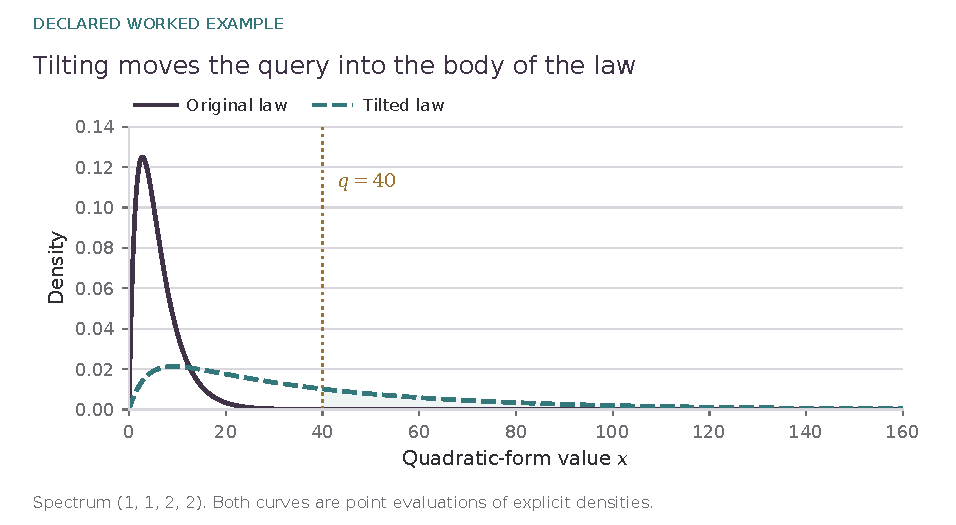
\includegraphics[width=\linewidth]{figures_production/worked_tilt.pdf}
\caption{The running example before and after exponential tilting. The original mean is $6$, while the reweighted mean is the query $q=40$. Shading identifies the tail under the tilted law. Both curves are point evaluations of explicit densities, not numerical enclosures.}
\label{fig:worked-tilt}
\end{figure}

The two copies of $1$ form one exact packet, and the two copies of $2$ form another. All centered deviations vanish, so the packet remainder is zero on every admissible grid. The numerical enclosure still has support, Fourier-mode, and arithmetic errors.

\clearpage
\section{A packet with a nonzero remainder}\label{sec:worked-packet}
To see the approximation itself, take a separate declared packet
\[
\{1.96,1.98,2.02,2.04\},\qquad \mu=2,
\]
and evaluate its contribution at $s=0.1+0.4\,\mathrm i$. The deviations are $-0.04,-0.02,0.02,0.04$. In particular,
\[
M_1=M_3=0,\quad M_2=0.004,\quad M_4=0.00000544.
\]
The factor $\alpha=2s/(1-4s)$ gives $\rho=0.04|\alpha|<1$, so Theorem~\ref{thm:packet} applies. Retaining successive even moment orders gives the values below. Both columns are rounded point evaluations. The theorem, not these rounded comparisons, is the reason the remainder is bounded.

\begin{center}\small\begin{tabular}{rrr}\toprule Order & Point-evaluated error & Analytic bound\\\midrule
0 & $2.3289\times10^{-4}$ & $3.9366\times10^{-2}$\\
2 & $3.6881\times10^{-8}$ & $4.8893\times10^{-6}$\\
4 & $8.7572\times10^{-12}$ & $1.0931\times10^{-9}$\\
6 & $2.419\times10^{-15}$ & $2.9091\times10^{-13}$\\
8 & $7.1896\times10^{-19}$ & $8.4306\times10^{-17}$\\
10 & $2.2307\times10^{-22}$ & $2.5701\times10^{-20}$\\
\bottomrule\end{tabular}
\end{center}

\begin{figure}[!htbp]
\centering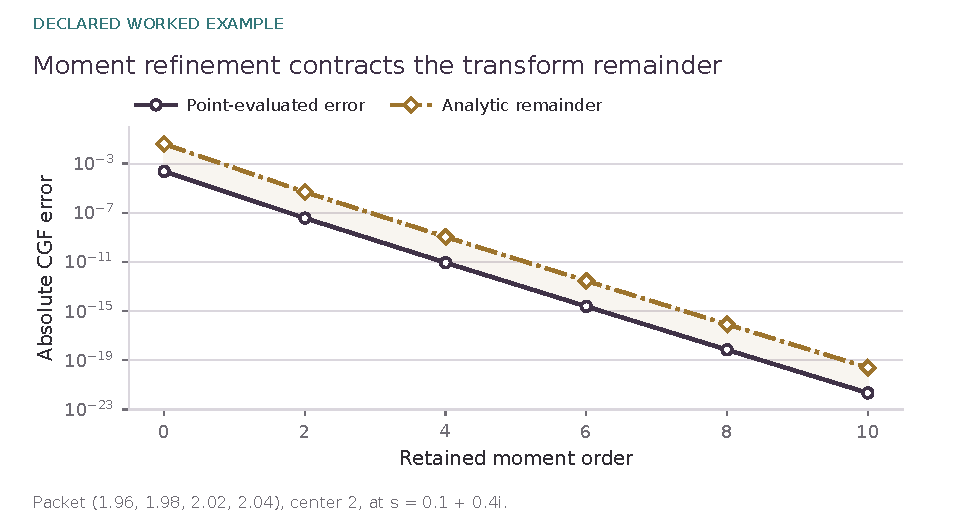
\includegraphics[width=\linewidth]{figures_production/worked_packet_error.pdf}
\caption{Pointwise transform error and its geometric remainder for the declared packet $(1.96,1.98,2.02,2.04)$ at $s=0.1+0.4i$. Increasing the retained moment order contracts both quantities. The shaded gap separates the observed discrepancy from the analytic bound.}
\label{fig:spectral-packets}
\end{figure}



\chapter{COS inversion and the analytic error budget}\label{ch:inversion}
\chapterlead{The tail functional has three distinct approximation errors: packet
compression on a finite grid, finite support with cosine folding, and omitted
Fourier modes. Each receives its own bound. Their sum yields an analytic
certificate, while a finite-refinement theorem shows that the mathematical
error can be made arbitrarily small for a fixed positive spectrum and an
upper-tail query.}
\section{Tilted COS tail functional}

Because $Q\ge0$, K-COS uses the interval $[0,b]$.  Throughout the
following functional and packet-error results, assume $b>q\ge0$, $b>0$,
$0<\theta<1/(2\lambda_{\max})$, and an integer mode count $N\ge1$.  Let
\[
u_k=\frac{k\pi}{b},
\qquad k=0,1,\ldots,
\]
and define the exponentially weighted cosine integrals
\begin{equation}
J_k(q,b,\theta)
=\int_q^b e^{-\theta(x-q)}\cos(u_kx)\,dx.
\label{eq:J-def}
\end{equation}
They admit the closed form
\begin{equation}
J_k
=\Re\left[
 e^{\ii u_k q}
 \frac{1-e^{(-\theta+\ii u_k)(b-q)}}{\theta-\ii u_k}
\right].
\label{eq:J-formula}
\end{equation}
The prime on a cosine sum denotes half weight for $k=0$.

If the exact tilted characteristic function is used, the $N$-mode finite-window expression is
\begin{equation}
T_{N,b}
=\frac{2}{b}\sum_{k=0}^{N-1}{}'
J_k\,
\Re\left[e^{\kappa(\theta+\ii u_k)-\theta q}\right].
\label{eq:tail-cos}
\end{equation}
The cancellation of $\kappa(\theta)$ in \eqref{eq:tail-cos} is useful numerically: the likelihood-ratio prefactor from \eqref{eq:tilt-tail} and the normalization in \eqref{eq:tilt-cf} do not need to be formed separately inside each mode.

\section{Propagation of packet error}

Let $\widehat\kappa(s_k)$ be the packet approximation at
\[
s_k=\theta+\ii u_k,
\]
and suppose
\begin{equation}
|\widehat\kappa(s_k)-\kappa(s_k)|\le B_k.
\label{eq:Bk}
\end{equation}
For disjoint packets, $B_k$ can be chosen as the sum of the packet bounds \eqref{eq:packet-remainder}.

\begin{theorem}[Finite-grid packet-to-tail bound]
\label{thm:packet-tail}
Let $\widehat T_{N,b}$ be obtained from \eqref{eq:tail-cos} by replacing $\kappa(s_k)$ by $\widehat\kappa(s_k)$. Then
\begin{equation}
|\widehat T_{N,b}-T_{N,b}|
\le \eps_{\mathrm{pkt}},
\label{eq:packet-tail-bound}
\end{equation}
where
\begin{equation}
\eps_{\mathrm{pkt}}
=
\frac{2}{b}
 e^{\kappa(\theta)-\theta q}
\sum_{k=0}^{N-1}{}'
|J_k|\bigl(e^{B_k}-1\bigr).
\label{eq:eps-pkt}
\end{equation}
\end{theorem}

\begin{proof}
Write $\Delta_k=\widehat\kappa(s_k)-\kappa(s_k)$. Then
\[
|e^{\widehat\kappa(s_k)-\theta q}-e^{\kappa(s_k)-\theta q}|
\le
|e^{\kappa(s_k)-\theta q}|\,(e^{|\Delta_k|}-1).
\]
Moreover
\[
\Re\kappa(\theta+\ii u_k)-\kappa(\theta)
=\log|\phi_{\theta}(u_k)|\le0,
\]
so
\[
|e^{\kappa(s_k)-\theta q}|
\le e^{\kappa(\theta)-\theta q}.
\]
Substitute this into the finite cosine sum and apply the triangle inequality.
\end{proof}

\section{Positive support, truncation, and cosine periodization}

Using full characteristic-function coefficients on $[0,b]$ reconstructs the even $2b$-periodization of the tilted density rather than the strictly truncated density. For a nonnegative density supported on $[0,\infty)$, the total mass folded back into $[0,b]$ equals the tilted mass above $b$. This gives a clean error control for the positive quadratic-form setting.


\begin{lemma}[Integrated cosine identity by folding]
\label{lem:folding}
Let \(\nu_\theta\) be the tilted probability measure and let
\(F_b:[0,\infty)\to[0,b]\) fold each interval of length \(2b\) by
reflection.  Then
\(\cos(k\pi F_b(x)/b)=\cos(k\pi x/b)\).
For \(h(x)=e^{-\theta(x-q)}\mathbf1_{[q,b]}(x)\),
\[
\int h\,d(F_{b\#}\nu_\theta)
=\frac2b\sum_{k=0}^{\infty}{}'
J_k\,\Re\phi_\theta(k\pi/b).
\]
The series is absolutely convergent for every positive rank \(r\ge1\).
\end{lemma}
\begin{proof}
A positive weighted chi-square sum has an absolutely continuous law. Its
folded measure therefore has no atom at the jump of \(h\).  The even periodic
extension of \(h\) has bounded Fej\'er means, which converge at every continuity
point.  Dominated convergence identifies the integral of those means with
\(\int h\,d(F_{b\#}\nu_\theta)\).  Their cosine coefficients are the Ces\`aro
weighted coefficients \(2J_k/b\), and folding preserves the cosine moments
\(\Re\phi_\theta(k\pi/b)\).  Finally
\(J_k=O(k^{-1})\) and
\(|\phi_\theta(k\pi/b)|=O(k^{-r/2})\), as follows directly from the product
formula below.  Thus the coefficient products are
\(O(k^{-1-r/2})\). Their absolute sum converges.  The Ces\`aro sums and ordinary
sum have the same limit, proving the displayed identity.  This argument
justifies the weighted functional without requiring pointwise convergence of
the reconstructed density at every boundary.
\end{proof}

\begin{proposition}[Support and periodization bound]
\label{prop:support}
Let the finite positive spectrum have rank \(r\ge1\), and let
\(b>q\ge0\), \(b>0\), and \(0<\theta<1/(2\lambda_{\max})\).  Let
\[
\tau_{\theta}(b)=\Pp_{\theta}(Q>b).
\]
Then the combined error from (i) replacing the tilted density on $[0,b]$ by its full-coefficient cosine periodization and (ii) omitting the original integral over $(b,\infty)$ is bounded by
\begin{equation}
\eps_{\mathrm{sup}}
\le
e^{\kappa(\theta)-\theta q}\,
\tau_{\theta}(b)
\left(1+e^{-\theta(b-q)}\right).
\label{eq:eps-support}
\end{equation}
\end{proposition}

\begin{proof}
By Lemma~\ref{lem:folding}, the infinite cosine functional integrates
the folded measure.  The part of that measure originating from \((b,\infty)\)
is nonnegative and has total mass $\tau_{\theta}(b)$. On $[q,b]$, the weight $e^{-\theta(x-q)}$ is at most one, so its contribution to the weighted functional is at most $\tau_{\theta}(b)$. For the omitted original tail, $x\ge b$ implies
\[
e^{-\theta(x-q)}\le e^{-\theta(b-q)},
\]
so that term is at most $e^{-\theta(b-q)}\tau_{\theta}(b)$. Multiplication by the likelihood-ratio prefactor in \eqref{eq:tilt-tail} gives \eqref{eq:eps-support}.
\end{proof}

The tilted tail probability itself can be bounded by Chernoff's inequality. For $\eta>\theta$ inside the transform domain,
\begin{equation}
\tau_{\theta}(b)
\le
\exp\left\{
\kappa(\eta)-\kappa(\theta)-(\eta-\theta)b
\right\}.
\label{eq:tilted-chernoff}
\end{equation}
When $b>\kappa'(\theta)$, the minimizing $\eta$ is the unique solution of
\begin{equation}
\kappa'(\eta)=b.
\label{eq:eta}
\end{equation}
For the saddlepoint tilt, $\kappa'(\theta_*)=q<b$, so such an $\eta$ exists.

\section{A specialized omitted-mode bound}

The tilted characteristic function has an especially transparent modulus.

\begin{lemma}[Tilted characteristic-function modulus]
\label{lem:modulus}
Define
\begin{equation}
a_j=\frac{2\lambda_j}{1-2\theta\lambda_j}>0.
\label{eq:aj}
\end{equation}
Then
\begin{equation}
|\phi_{\theta}(t)|
=\prod_{j=1}^{r}\left(1+(a_jt)^2\right)^{-1/4}.
\label{eq:phi-modulus}
\end{equation}
For $t>0$, define the logarithmic decay rate
\begin{equation}
\beta(t)
=-\frac{d\log|\phi_{\theta}(t)|}{d\log t}
=\frac12\sum_{j=1}^{r}
\frac{(a_jt)^2}{1+(a_jt)^2}.
\label{eq:beta}
\end{equation}
Set $\beta(0)=0$ by continuous extension. Then $\beta(t)$ is nondecreasing for $t\ge0$.
\end{lemma}

\begin{proof}
Taking the modulus of each factor in \eqref{eq:tilt-cf} gives \eqref{eq:phi-modulus}. Differentiating its logarithm gives \eqref{eq:beta}. Each summand $x/(1+x)$ with $x=(a_jt)^2$ is nondecreasing in $t$.
\end{proof}

\begin{corollary}[Power envelope from one frequency]
\label{cor:power-envelope}
For $t\ge t_0>0$,
\begin{equation}
|\phi_{\theta}(t)|
\le
|\phi_{\theta}(t_0)|
\left(\frac{t}{t_0}\right)^{-\beta(t_0)}.
\label{eq:power-envelope}
\end{equation}
\end{corollary}

\begin{proof}
By Lemma \ref{lem:modulus},
\[
\frac{d\log|\phi_{\theta}(t)|}{d\log t}=-\beta(t)\le-\beta(t_0)
\]
for $t\ge t_0$. Integrating from $t_0$ to $t$ proves the claim.
\end{proof}

For $k\ge1$, the exact integral \eqref{eq:J-formula} implies
\begin{equation}
|J_k|
\le \frac{2}{u_k}.
\label{eq:J-bound}
\end{equation}

\begin{theorem}[Omitted COS-mode certificate]
\label{thm:cos-tail}
Let $N\ge1$ and $b>q\ge0$. Set $u_N=N\pi/b$ and
$\beta_N=\beta(u_N)$. If $\beta_N>0$, then the contribution of all exact tilted-COS modes $k\ge N$ to the weighted tail functional is bounded by
\begin{equation}
\eps_{\mathrm{COS}}
\le
 e^{\kappa(\theta)-\theta q}
\frac{4|\phi_{\theta}(u_N)|}{\pi}
\left(\frac1N+\frac1{\beta_N}\right).
\label{eq:eps-cos}
\end{equation}
\end{theorem}

\begin{proof}
Using the cosine coefficient magnitude $2|\phi_{\theta}(u_k)|/b$ and \eqref{eq:J-bound}, the omitted series is at most
\[
e^{\kappa(\theta)-\theta q}
\frac{4}{\pi}
\sum_{k=N}^{\infty}\frac{|\phi_{\theta}(u_k)|}{k}.
\]
By Corollary \ref{cor:power-envelope},
\[
|\phi_{\theta}(u_k)|
\le
|\phi_{\theta}(u_N)|\left(\frac{k}{N}\right)^{-\beta_N}.
\]
Therefore
\[
\sum_{k=N}^{\infty}\frac{|\phi_{\theta}(u_k)|}{k}
\le
|\phi_{\theta}(u_N)|N^{\beta_N}
\sum_{k=N}^{\infty}k^{-\beta_N-1}.
\]
Finally,
\[
\sum_{k=N}^{\infty}k^{-\beta_N-1}
\le N^{-\beta_N-1}+\int_N^{\infty}x^{-\beta_N-1}\,dx
=N^{-\beta_N-1}+\frac{N^{-\beta_N}}{\beta_N},
\]
which yields \eqref{eq:eps-cos}.
\end{proof}

\section{Combined analytic certificate}

\begin{theorem}[K-COS analytic error certificate]
\label{thm:combined}
Let $p=\Pp(Q\ge q)$, and let $\widehat p$ be the finite K-COS approximation formed with
\begin{enumerate}[label=(\roman*)]
\item an upper interval endpoint $b>q$,
\item an integer $N\ge1$ of cosine modes,
\item a packet approximation satisfying \eqref{eq:Bk} on the finite grid.
\end{enumerate}
Under the positive-spectrum and parameter hypotheses of Proposition \ref{prop:support},
\begin{equation}
|p-\widehat p|
\le
\eps_{\mathrm{an}}
:=\eps_{\mathrm{pkt}}+\eps_{\mathrm{sup}}+\eps_{\mathrm{COS}}.
\label{eq:combined}
\end{equation}
If $\eps_{\mathrm{an}}<|\widehat p|$, then
\begin{equation}
\frac{|p-\widehat p|}{|p|}
\le
\frac{\eps_{\mathrm{an}}}
{|\widehat p|-\eps_{\mathrm{an}}}.
\label{eq:relative-certificate}
\end{equation}
\end{theorem}

\begin{proof}
Decompose the error into packet error on the retained grid, support and periodization error, and the exact omitted cosine series. The first is bounded by Theorem \ref{thm:packet-tail}, the second by Proposition \ref{prop:support}, and the third by Theorem \ref{thm:cos-tail}. This proves \eqref{eq:combined}. Also
\[
|p|\ge |\widehat p|-|p-\widehat p|
\ge |\widehat p|-\eps_{\mathrm{an}},
\]
which gives \eqref{eq:relative-certificate}.
\end{proof}

\begin{remark}[Certificate boundary]\label{claim:final-26-12}
Theorem \ref{thm:combined} is an \emph{analytic approximation certificate}. It does not enclose IEEE floating-point rounding in complex logarithms, exponentials, root finding, or summation. A machine-level certificate would require directed rounding, interval arithmetic, or a comparable validated-numerics layer.
\end{remark}

\section{Finite refinability}

The combined error terms correspond to three distinct obstructions. Packet error is reduced by splitting spectral packets or raising packet order. Support error is reduced by increasing $b$. Cosine-series error is reduced by increasing $N$.

\begin{proposition}[Existence of a finite analytic refinement]
\label{prop:finite-refinement}
Fix a finite positive spectrum $\{\lambda_j\}_{j=1}^{r}$, an upper-tail query $q>\E Q$, and $\eps>0$. There exist a finite interval endpoint $b>q$, a finite number of cosine modes $N$, and a finite packet partition (allowing singleton packets) for which the analytic error bound in \eqref{eq:combined} is below $\eps$.
\end{proposition}

\begin{proof}
First choose $b$ sufficiently large that \eqref{eq:eps-support} is below $\eps/3$. This is possible because the tilted law has a moment generating function in a nontrivial right neighborhood of zero and hence its Chernoff bound tends to zero exponentially as $b\to\infty$. Hold this $b$ fixed. By \eqref{eq:phi-modulus}, $|\phi_{\theta}(t)|\to0$ polynomially as $t\to\infty$, while $\beta(t)\to r/2>0$. Therefore \eqref{eq:eps-cos} tends to zero as $N\to\infty$, so a finite $N$ makes it below $\eps/3$. Finally, split every packet to singletons if necessary. A singleton has $\delta_j=0$, so its packet remainder is exactly zero. Hence a finite partition makes $\eps_{\mathrm{pkt}}<\eps/3$. Summing the three terms proves the claim.
\end{proof}

\begin{remark}\label{claim:final-26-14}
Proposition \ref{prop:finite-refinement} proves existence of a finite representation meeting any analytic tolerance. It proves neither termination of an arbitrary greedy schedule nor optimality of its resource use. A particular capped implementation can fail to certify even though a finite analytic refinement exists. The packet planner refines the largest currently certified obstruction and is evaluated in Chapter~\ref{ch:evidence}.
\end{remark}



\chapter{Adaptive evaluation and numerical interfaces}\label{ch:adaptive}
\chapterlead{An adaptive solver should refine the representation responsible for the
largest unresolved error. The planner described here chooses packets, support,
and modes jointly. Its floating implementation retains an analytic ledger.
The next part supplies the stricter contract in which finite arithmetic and
output serialization are enclosed as well.}
\section{Adaptive K-COS algorithm}

The packet planner accepts a finite positive spectrum, an upper-tail query
$q>\sum_j\lambda_j$, and a requested relative tolerance $\tau>0$.
Its initial support parameter satisfies $L>0$, and its mode count is a
positive integer.

\begin{enumerate}[leftmargin=2em]
\item Solve $\kappa'(\theta_*)=q$.
\item Initialize an upper interval $b=q+L\sqrt{\kappa''(\theta_*)+\sqrt{\kappa^{(4)}(\theta_*)}}$ and a mode count $N$.
\item Retain the largest spectral spikes exactly and place the remaining sorted eigenvalues into coarse packets.
\item Evaluate $\rho_P(\theta_*+\ii u_k)$ and the packet remainder bound on the actual COS grid. Split packets until the propagated packet contribution is within its budget.
\item Evaluate the support/alias certificate from \eqref{eq:eps-support}--\eqref{eq:eta}.
\item Evaluate the omitted-mode certificate \eqref{eq:eps-cos}.
\item If the combined relative certificate exceeds $\tau$, refine whichever analytic error source dominates: split packets, increase $b$, or increase $N$.
\item Return a certified analytic result only after the combined bound meets
$\tau$. Return the tail estimate, the compiled spectral representation,
and its error ledger together. If resource limits are reached first,
report failure to certify rather than accepting the estimate.
\end{enumerate}

The resulting object is query dependent. Schematically,
\begin{equation}
(\Lambda,q,\tau)
\longmapsto
\mathcal P_{\Lambda,q,\tau}
\longmapsto
(\widehat p,\text{certificate}),
\label{eq:compiler-map}
\end{equation}
where $\mathcal P_{\Lambda,q,\tau}$ stores exact spikes, packet centers, centered moments, packet radii, and the selected COS parameters.


\section{Numerical interfaces and log-domain evaluation}\label{sec:final-25}

The preceding mathematics is exposed through a domain-neutral engine rather
than through a SKAT-only entry point.  The central positive engine accepts:

\begin{itemize}
\item an explicit nonnegative spectrum.
\item a positive semidefinite matrix.
\item a dense factor \(A\).
\item a replayable streamed column-factor source.
\item or a covariance/quadratic-matrix pair
\((\Sigma,M)\).
\end{itemize}

A signed central engine accepts a signed spectrum, a symmetric operator, or
\[
(\Sigma,M),\qquad M=M^\top,
\]
and performs the exact central-indefinite reduction proved in Chapter~\ref{ch:gaussian}.  A
separate noncentral positive engine accepts
\[
(\mu,\Sigma,M),\qquad M\succeq0,
\]
and performs the corresponding noncentral reduction.

\subsection{Log-domain packet error accumulation}

After separating the likelihood-ratio prefactor, the packet contribution
contains sums of the form
\[
\frac{2}{b}
\sum_k
|J_k|
\left(
e^{\varepsilon_k}-1
\right).
\]
Direct evaluation can overflow even when the candidate is destined to be
rejected by the adaptive planner.  The implementation instead
computes
\[
\log\left(
\frac{2}{b}
\sum_k
|J_k|
\left(
e^{\varepsilon_k}-1
\right)
\right)
\]
by log-sum-exp arithmetic, and compares this quantity with the logarithm of
the requested tolerance before converting a final accepted bound back to
float64.

This change does not weaken the mathematical bound. It changes only its
floating-point representation.

\subsection{Reference convergence is part of verification}

An independently evaluated reference is useful only if its own numerical
resolution has converged.  In a rank-350 deep-tail audit, an initial fixed-grid
reference appeared to disagree with the adaptive answer.  Increasing the reference COS grid gave absolute discrepancies of approximately
\[
1.88\times10^{-2},
\quad
2.6\times10^{-3}\text{--}4.0\times10^{-3},
\quad
1.39\times10^{-4},
\quad
2.60\times10^{-8}
\]
decades as the grid was refined through
\[
N=4096,\ 8192,\ 16384,\ 32768.
\]

\begin{figure}[htbp]
\centering
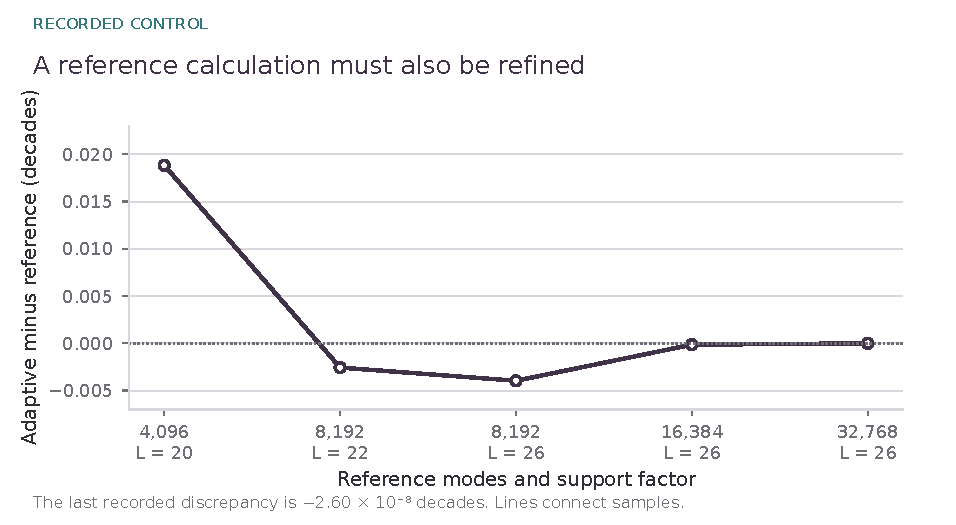
\includegraphics[width=\linewidth]{figures_production/figure_21_reference_convergence.pdf}
\caption{The adaptive result is compared with progressively refined full-spectrum references. The reference discrepancy is not monotone across the intermediate grids. Its final recorded value is approximately $-2.60\times10^{-8}$ decades, illustrating why a reference needs its own convergence check.}
\label{fig:reference-convergence}
\end{figure}

The numerical verification rule is consequently two-sided: the adaptive
solver must satisfy its own certificate, and any external or fixed-grid
reference used for comparison must demonstrate numerical convergence.




\monopart{part:certified}{Certified numerical computation}{A remainder theorem concerns exact arithmetic. A numerical enclosure must also contain the arithmetic used to evaluate the approximation. This part connects those obligations, states the acceptance rule, and examines the evidence and limits of the implementation.}
\chapter{Directed probability enclosures}\label{ch:intervals}

\label{sec:final-4}

\chapterlead{An analytic remainder estimate controls the error of a mathematical
approximation. A numerical enclosure must also control the arithmetic used
to evaluate it. This chapter joins directed arithmetic to explicit
remainder bounds, yielding an interval for an exactly supplied positive
spectrum under the stated arithmetic trust assumptions.}

The notation follows the analytic development: $\kappa$ is the cumulant generating function, $b$ the support endpoint, $N$ the retained mode count, and $J_k$ the payoff coefficient. The implementation-name correspondence is given in Appendix~\ref{app:reproduction}.

\section{Interval target}

For a positive central quadratic form
\[
Q=\sum_{j=1}^{r}\lambda_jZ_j^2,
\qquad
\lambda_j>0,
\]
the output is not merely a point estimate.  It is
\[
\boxed{
\log_{10}P(Q\ge q)\in[d_-,d_+].
}
\]
Hence the corresponding multiplicative uncertainty satisfies
\[
\boxed{
\frac{p_+}{p_-}\le 10^{d_+-d_-}.
}
\]

The finite transform and exponential prefactor are evaluated by
directed-rounding interval arithmetic.  The resulting interval is enlarged by
two independently proved analytic remainders: a support/periodization alias
bound and an omitted-COS-mode bound.

\section{No exact saddlepoint is required}

Choose any
\[
0<\theta<\frac{1}{2\lambda_{\max}}.
\]
Exponential tilting gives
\[
P(Q\ge q)
=
e^{\kappa(\theta)-\theta q}
S_\theta(q),
\]
where
\[
S_\theta(q)
=
E_\theta\!\left[
e^{-\theta(Q-q)}
1_{\{Q\ge q\}}
\right].
\]

The interval proof does not require \(\theta\) to be the exact saddlepoint.
A high-precision saddlepoint is used only as an efficient design choice.
Once serialized as an exact decimal input, it is simply a valid tilt inside
the MGF domain.

The same is true of the support endpoint \(b\) and the auxiliary Chernoff
parameter \(\eta\).  Correctness requires only
\[
b>q\ge0,\qquad b>0,
\qquad
\theta<\eta<\frac{1}{2\lambda_{\max}}.
\]

\section{Rigorous support and alias control}

Under the tilted measure,
\[
P_\theta(Q>b)
\le
\exp\left\{
\kappa(\eta)-\kappa(\theta)-(\eta-\theta)b
\right\}.
\]

The full-characteristic-function cosine expansion periodizes the tilted density
on \([0,b]\).  Because the original positive quadratic form is supported on
\([0,\infty)\), the total positive-tail mass aliased back into one fundamental
interval is at most \(P_\theta(Q>b)\).

The actual payoff omitted above \(b\) is at most
\[
e^{-\theta(b-q)}P_\theta(Q>b).
\]

Therefore
\[
\boxed{
E_{\rm support}
\le
P_\theta(Q>b)
\left(
1+e^{-\theta(b-q)}
\right).
}
\]

\section{Rigorous infinite-mode control}

Define
\[
a_j=
\frac{2\lambda_j}{1-2\theta\lambda_j}.
\]
The normalized tilted characteristic function satisfies
\[
|\phi_\theta(t)|
=
\prod_{j=1}^r
\left(
1+(a_jt)^2
\right)^{-1/4}.
\]

Since
\[
1+(a_jt)^2\ge(a_jt)^2,
\]
we have
\[
|\phi_\theta(t)|
\le
C_\theta t^{-r/2},
\qquad
C_\theta=\prod_j a_j^{-1/2}.
\]

For the payoff coefficient
\[
J_k=
\int_q^b
e^{-\theta(x-q)}
\cos(k\pi x/b)\,dx,
\]
the elementary bound
\[
|J_k|\le\frac1\theta
\]
holds.

Let
\[
\nu=\frac r2>1,\qquad N\ge1.
\]
For a finite transform retaining modes \(0,\ldots,N-1\),
\[
\boxed{
E_{\rm series}
\le
\frac{2C_\theta}{b\theta}
\left(\frac{b}{\pi}\right)^\nu
\left[
N^{-\nu}
+
\frac{N^{1-\nu}}{\nu-1}
\right].
}
\]

This implemented interval backend therefore requires \(r>2\).  Lower-rank positive
forms can use a different tail bound and are not claimed by this theorem.

\section{Final enclosure theorem}

Let \(\boldsymbol S_N\) be the directed-rounding interval containing the finite
\(N\)-mode tilted COS sum, and set
\[
E=E_{\rm support}+E_{\rm series}.
\]
Then
\[
\boxed{
S_\theta(q)
\in
\boldsymbol S_N+[-E,E].
}
\]

If the lower endpoint of this interval is positive, directed rounding gives
\[
\boxed{
\log P(Q\ge q)
\in
\kappa(\theta)-\theta q
+
\log\left(
\boldsymbol S_N+[-E,E]
\right).
}
\]

All finite arithmetic in this expression is enclosed by the interval backend.

\section{Completing the running calculation}\label{sec:worked-enclosure}
The factor, spectrum, and tilt of Sections~\ref{sec:worked-law}--\ref{sec:worked-tilt} now determine a complete positive-spectrum calculation at $q=40$. The exact diagonalization supplies the coefficients $(1,1,2,2)$. The implementation receives those coefficients as exact decimal literals, together with a serialized decimal approximation to the admissible tilt. Correctness does not require that decimal to equal the radical saddlepoint exactly.

With $b=512$, $N=16384$, auxiliary tilt $\eta=0.245$, and 60 interval decimal digits, the supplied backend returns a logarithmic interval. Rounding its lower endpoint downward and its upper endpoint upward gives the readable enclosure
\[
\log_{10}P(Q\ge40)\in\bigl[-4.04489575,-4.03897381\bigr].
\]
At $N=8192$, the directed ratio upper bound is approximately $0.0246131$, which fails the requested tolerance $0.02$. Doubling the retained mode count, rather than relaxing the tolerance, gives the interval above. The full serialized interval has a directed multiplicative ratio upper bound below $0.013731$. The displayed, coarser interval also meets the requested tolerance $0.02$. An independently evaluated interval for the exact expression $2e^{-10}-e^{-20}$ lies entirely inside the COS enclosure.

This same fixed enclosure does not meet tolerance $0.001$. The acceptance routine rejects that tighter request. This is an intended distinction between an accurate point estimate and an established enclosure width. The rank-four example has slower Fourier decay than the rank-eighty control developed later, so its mode count should not be interpreted as a general cost prediction.


\begin{figure}[!htbp]
\centering
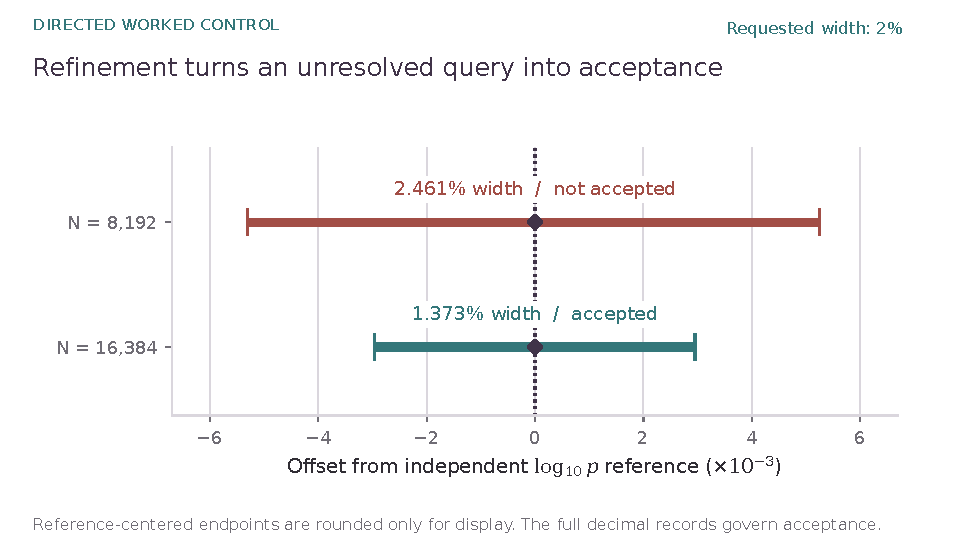
\includegraphics[width=\linewidth]{figures_production/worked_enclosure_refinement.pdf}
\caption{The running example under a requested multiplicative width of $2\%$. Increasing the mode count narrows the directed interval from a failing width of approximately $2.461\%$ to a passing width of approximately $1.373\%$. Diamonds mark the independent closed-form reference. The reference-centered axis is rounded for display only.}
\label{fig:worked-enclosure-refinement}
\end{figure}

The certificate in this example concerns the tail evaluation for the exact spectrum. Its connection to the matrix is the explicit algebraic diagonalization above. It does not test a black-box eigensolver. Chapter~\ref{ch:spectrum} gives the separate post-verification theorem required for a general computed eigensystem.

\section{Independent exact interval control through \texorpdfstring{\(10^{-5000}\)}{1e-5000}}

For the control
\[
Q=0.02\chi^2_{80},
\]
the survival probability has the finite exact formula
\[
P(Q\ge q)
=
e^{-x}
\sum_{j=0}^{39}
\frac{x^j}{j!},
\qquad
x=\frac{q}{0.04}.
\]

This finite expression was evaluated independently by directed-rounding
interval arithmetic, without using K-COS.  The K-COS enclosure and this exact
control enclosure are compared at thresholds targeting
\[
p\approx10^{-100},
\qquad
10^{-1000},
\qquad
10^{-5000}.
\]

With $N=128$ and 90 interval decimal digits, the resulting K-COS widths
are listed below. Widths and ratios are computed from the full outward
endpoints before rounding the displayed values. At all three stored inputs,
the independent exact-law interval is fully contained in the K-COS interval.

\begin{center}
\begin{tabular}{@{}rrr@{}}
\toprule
target & width in $\log_{10}p$ & multiplicative ratio minus one\\
\midrule
$10^{-100}$ &
$8.93\times10^{-13}$ &
$2.06\times10^{-12}$\\
$10^{-1000}$ &
$7.01\times10^{-12}$ &
$1.62\times10^{-11}$\\
$10^{-5000}$ &
$3.34\times10^{-11}$ &
$7.70\times10^{-11}$\\
\bottomrule
\end{tabular}
\end{center}

Thus the \(10^{-5000}\) result is not merely a point estimate agreeing with a
reference.  For the exact supplied spectrum, it comes with a directed-rounding
logarithmic enclosure whose probability ratio satisfies
\[
\boxed{
\frac{p_+}{p_-}
\le
1+7.70\times10^{-11}
}
\]
The displayed upper bound is rounded upward from the directed ratio bound.

\begin{figure}[htbp]
\centering
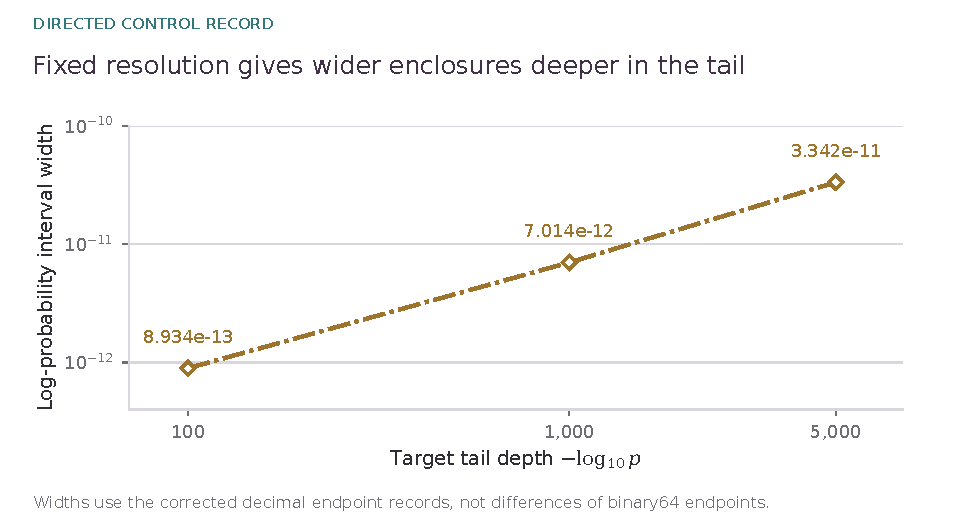
\includegraphics[width=\linewidth]{figures_production/figure_24_interval_deep_tail_width.pdf}
\caption{Directed log-probability widths on exact scaled-chi-square controls at fixed $N=128$ and 90 interval digits. Values come from the corrected full decimal endpoint records. Subtracting rounded binary64 endpoints would give a different diagnostic.}
\label{fig:interval-tail-width}
\end{figure}




\section{Arithmetic width versus analytic width}

At the \(10^{-5000}\) control, the interval precision was swept from 40 to 120
decimal digits.  The total certified width remained essentially
\[
3.34247\times10^{-11}
\]
decades.

Over the same sweep, the arithmetic-only width contracted from approximately
\[
7.5\times10^{-37}
\]
to
\[
6.3\times10^{-117}
\]
decades.

\begin{figure}[htbp]
\centering
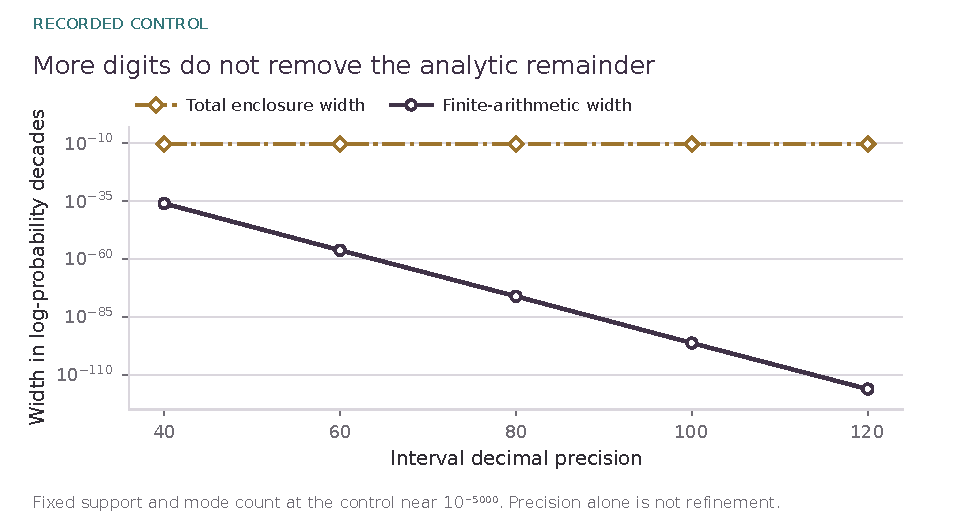
\includegraphics[width=\linewidth]{figures_production/figure_25_interval_arithmetic_vs_analytic.pdf}
\caption{Increasing interval precision suppresses finite-arithmetic width but leaves the analytic remainder essentially unchanged at fixed support and mode count. Both quantities are shown separately for the control near $10^{-5000}$. More digits alone cannot remove a truncation error.}
\label{fig:interval-arithmetic}
\end{figure}

This separation is important.  Increasing numerical precision cannot improve
an analytic truncation theorem.  Conversely, once interval arithmetic is far
below the analytic error budget, numerical rounding is no longer the limiting
uncertainty.

\section{Guarantee boundary}

The directed enclosure has the following scope:

\begin{quote}
For an exact supplied positive decimal spectrum of rank greater than two, the
backend returns a directed-rounding logarithmic probability enclosure enlarged
by proved analytic support/alias and omitted-mode bounds.
\end{quote}

The result is conditional on correctness of the interval-arithmetic library
implementation.  The implementation uses \texttt{mpmath.iv}, whose
interval layer applies downward and upward endpoint rounding.

A completely end-to-end guarantee beginning from an arbitrary floating-point
matrix requires one more layer: either a rigorously enclosed matrix-to-spectrum
computation, or an exact/residual completion step whose linear algebra is also
performed with verified interval or ball arithmetic.

The supplied interval backend evaluates the exact spectrum directly.
Packet centers, moments, and their propagated errors are not evaluated with
directed arithmetic in this implementation. The packetized path therefore
retains its separate analytic guarantee.




\chapter{Accuracy-driven certification}\label{ch:accuracy}
\chapterlead{A requested tolerance is an input to the problem, not an informal expectation
about its answer. The controller accepts a result only when an outward
probability interval proves the multiplicative accuracy requirement. Failure
to prove that inequality remains a failure of certification, even when a
point estimate appears accurate.}
\label{sec:final-5}

The external numerical contract specifies the desired accuracy, not the
internal transform resolution.

For an exact positive spectrum and threshold \(q\), the solver accepts a
requested relative multiplicative accuracy
\[
\varepsilon_{\rm req}>0
\]
and returns a certified interval
\[
[p_-,p_+]
\]
only when
\[
\boxed{
\frac{p_+}{p_-}-1
\le
\varepsilon_{\rm req}.
}
\]

In logarithmic coordinates, if
\[
\log_{10}p\in[d_-,d_+],
\]
the acceptance rule is
\[
\boxed{
10^{d_+-d_-}-1
\le
\varepsilon_{\rm req}.
}
\]

No value of \(N\), support width, or arithmetic precision appears in the
external contract.

\begin{theorem}[Accuracy contract for the positive exact-spectrum backend]\label{claim:final-5-1}
Assume an exact supplied positive decimal spectrum of rank greater than two,
a threshold \(q\ge0\) with valid interval-design parameters, and requested multiplicative tolerance
\(\varepsilon_{\rm req}>0\).  Suppose the directed-rounding interval backend
returns an enclosure
\[
\log_{10}p\in[d_-,d_+]
\]
that includes the proved support/alias and omitted-mode remainders.  If the
accuracy-driven controller returns \texttt{certified=True}, then
\[
\boxed{
P(Q\ge q)\in[10^{d_-},10^{d_+}]
}
\]
and
\[
\boxed{
\frac{10^{d_+}}{10^{d_-}}-1
\le
\varepsilon_{\rm req}.
}
\]
If the resource caps are reached before this inequality is proved, the
controller returns \texttt{certified=False} rather than promoting the interval
midpoint to a certified answer.
\end{theorem}

\begin{proof}
The directed-rounding backend encloses the finite transform and exponential
prefactor and then enlarges that enclosure by the proved support/alias and
infinite-mode error bounds.  Therefore the true tail probability lies inside
the returned interval.  The controller encloses
\(\operatorname{expm1}(\log(10)(d_+-d_-))\) by directed rounding and
sets \texttt{certified=True} only when the upper endpoint of that ratio
enclosure is no larger than the lower endpoint of the exact requested
tolerance enclosure.  High precision alone is not an enclosure proof.  The fail-closed branch follows directly from
the controller definition.
\end{proof}

\section{Adaptive refinement}

The controller adjusts three internal resources:

\begin{enumerate}
\item the COS mode count \(N\).
\item the tilted support scale \(L\), which changes \(b\) and its associated
Chernoff parameter.
\item the interval arithmetic precision.
\end{enumerate}

At each stage the full directed-rounding interval is recomputed.  If the
rounding component is material relative to the requested budget, arithmetic
precision is increased.  Otherwise the dominant analytic contribution
determines the next refinement: mode error increases \(N\), while
support/alias error increases \(L\).

A certified return occurs only after the multiplicative inequality above
has been proved. Reaching a resource limit instead terminates the calculation
with the failure status described next.

\section{Fail-closed behavior}

If the configured resource caps are exhausted before the requested accuracy
is established, the solver does not silently return its midpoint as though it
were certified.

Instead it returns
\[
\boxed{\texttt{certified = false}}
\]
together with the unresolved interval and a failure reason.

This behavior is part of the numerical definition of the solver.

\section{Accuracy ladder through \texorpdfstring{\(10^{-5000}\)}{1e-5000}}

The exact control
\[
Q=0.02\chi^2_{80}
\]
was evaluated at tail depths
\[
10^{-100},
\qquad
10^{-1000},
\qquad
10^{-5000}.
\]

For each depth the controller was asked to prove relative multiplicative
accuracies
\[
10^{-8},
\quad
10^{-10},
\quad
10^{-12},
\quad
10^{-14}.
\]
All twelve contracts were satisfied.

At the \(10^{-5000}\) point, the controller produced:

\begin{center}
\begin{tabular}{@{}rrrr@{}}
\toprule
requested accuracy & achieved ratio minus one & \(N\) & \(L\)\\
\midrule
\(10^{-8}\)  & \(3.19\times10^{-10}\) & 64  & 10\\
\(10^{-10}\) & \(7.70\times10^{-11}\) & 128 & 10\\
\(10^{-12}\) & \(3.48\times10^{-15}\) & 128 & 12\\
\(10^{-14}\) & \(3.48\times10^{-15}\) & 128 & 12\\
\bottomrule
\end{tabular}
\end{center}

The gap between requested and achieved accuracy is expected: refinement is
discrete, so one additional support or mode refinement can improve the
certificate by several orders of magnitude.

A further stress test requested
\[
10^{-16}
\quad\text{and}\quad
10^{-18}
\]
relative accuracy at the same \(10^{-5000}\) tail.  The solver obtained
approximately
\[
3.05\times10^{-18}
\]
and
\[
9.20\times10^{-20}
\]
respectively.

\begin{figure}[htbp]
\centering
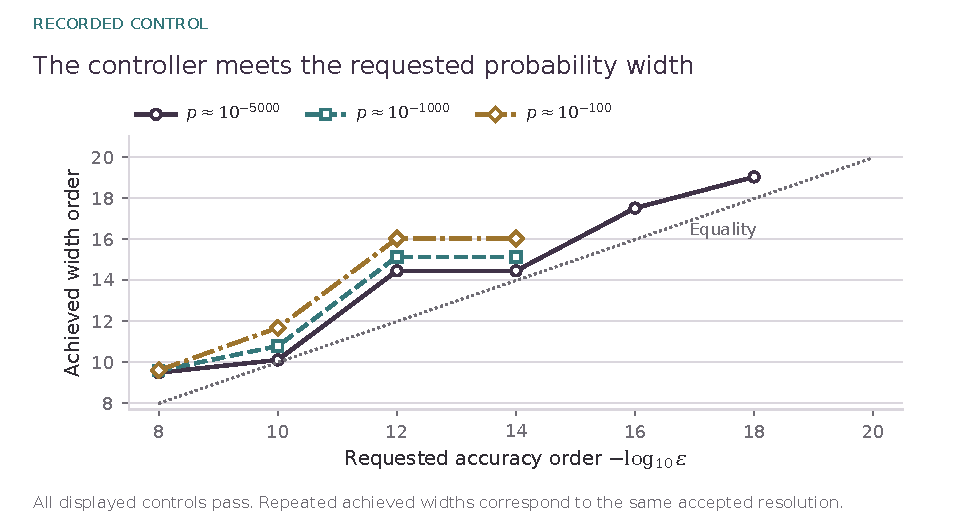
\includegraphics[width=\linewidth]{figures_production/figure_26_accuracy_driven_refinement.pdf}
\caption{Requested and achieved multiplicative widths, expressed as decimal accuracy orders. Larger values mean tighter widths, so points above the equality line meet the requested tolerance. The two deepest stress results use the rounded numerical summaries in the text. Acceptance itself uses the full directed endpoints.}
\label{fig:accuracy-driven}
\end{figure}

\section{Acceptance arithmetic and serialization are directed}

The acceptance condition must be evaluated as carefully as the probability
interval.

Converting a tiny log-width \(w\) using
\[
10^w-1
\]
under an insufficient point-precision context can lose the width. At approximately \(10^{-15}\)
relative scales, the ratio can round to zero.

Even when the probability interval remains valid, that conversion cannot
support a certification decision. The implementation encloses
\[
\boxed{
\operatorname{expm1}(\log(10)\,w)
}
\]
with directed interval arithmetic before deciding whether the requested
accuracy has been met.  Acceptance compares the upper endpoint of that ratio
with the lower endpoint of the requested exact tolerance, so a rounded point
estimate cannot promote an unresolved boundary case to success.

Authoritative output strings must preserve the same outer enclosure.  The
implementation converts each exact binary interval endpoint to a decimal
string with \texttt{Decimal} and explicit \texttt{ROUND\_FLOOR} for lower
endpoints or \texttt{ROUND\_CEILING} for upper endpoints.  Ordinary interval
display formatting is not used as an authoritative serialization method:
nearest-rounded decimal text can move an endpoint inward even when the
internal interval arithmetic was directed.  Matrix-to-tail propagation keeps
these endpoint strings and applies the same directed ratio test.

The correctness requirement applies not only to the tail integral but also
to the logic that labels its result certified.

\section{Input semantics at \texorpdfstring{\(p\approx10^{-16}\)}{p about 1e-16}}

At this accuracy scale, the representation of the threshold \(q\) itself is
measurable.  In the \(0.02\chi^2_{80}\) control targeted at \(10^{-16}\),
rounding the high-precision threshold to binary float64 shifts the exact tail
by approximately
\[
3.83\times10^{-15}
\]
decades.  The binary64 solver evaluated at that same rounded input
then differs from the exact tail of the rounded input by approximately
\[
5.17\times10^{-15}
\]
decades.

Accordingly, claims below the float64 input-quantization scale use exact-decimal
or interval inputs.  The rigorous accuracy contract therefore certifies the
mathematical inputs supplied to it, rather than silently identifying a rounded
binary threshold with an ideal decimal threshold.




\chapter{Numerical evidence and applications}\label{ch:evidence}
\chapterlead{Exact-law controls test values against independent formulas. Heterogeneous
spectra test inversion across irregular coefficients. Simulated kernels test
the operator pipeline. Timing measurements characterize particular
implementations. These are distinct forms of evidence.}
The source package records the inputs and environments behind the reported
experiments. The release regression and containment checks are reported in
Appendix~\ref{app:reproduction}.

\section{Deep-tail controls}\label{sec:final-3}
A directed enclosure includes rounding as well as analytic remainders. An analytic ledger evaluated in ordinary floating point does not. The labels in this chapter identify which conclusion a result supports. The retained timing measurements are not presented as a new hardware comparison.

The method is designed for a regime in which direct survival probabilities can
underflow long before the mathematical probability becomes numerically
unresolvable.  The engine therefore treats \(\log p\) as the primary numerical
quantity and evaluates its error bounds on that logarithmic scale.

The validation ladder spans seven qualitatively different settings:

\begin{center}
\small
\begin{tabular}{@{}P{0.27\linewidth}P{0.13\linewidth}P{0.22\linewidth}P{0.16\linewidth}P{0.12\linewidth}@{}}
\toprule
validation regime & deepest $\log_{10}p$ & observed error & certificate & spectral size\\
\midrule
directed-rounding $0.02\chi^2_{80}$ control
& $-5000$ & enclosure width $3.34\times10^{-11}$ decades
& multiplicative ratio $\le 1+7.70\times10^{-11}$ & 80 df\\
large-scale positive spectrum
& $-922.031162$ & below stored reference resolution & $5.71\times10^{-9}$ & rank 1997\\
strong-dependence kernel
& $-457.973916$ & below stored reference resolution & $5.20\times10^{-9}$ & rank 996\\
heterogeneous inversion benchmark near $10^{-16}$
& $-16$ & $2.88$--$6.52\times10^{-15}$ decades & independent integral converged & ranks 80--120\\
signed finite-endpoint exact control
& $-200$ & $\le 2.84\times10^{-14}$ decades & $7.23\times10^{-13}$ & rank 80\\
signed mixed multiscale
& $-81.891937$ & $1.42\times10^{-12}$ decades vs full grid & $5.78\times10^{-9}$ & rank 340\\
noncentral exact controls
& $-40$ & $\le 9.26\times10^{-15}$ decades & passing & up to 50 df\\
\bottomrule
\end{tabular}
\end{center}

The analytic scaled-chi-square ladder also includes
\[
\log_{10}p=-100,-300,-1000,-5000,
\]
with respective reported absolute log-probability discrepancies
\[
2.84\times10^{-14},\quad
<10^{-15},\quad
3.41\times10^{-13},\quad
<10^{-15}
\]
in the stored benchmark output.  The corresponding analytic relative certificates
remain finite throughout, reaching only
\[
3.85\times10^{-11}
\]
at \(10^{-5000}\).

A large-scale run with \(n=2000\), \(m=50{,}000\), 49,951 retained
features, and quadratic-form rank 1997 produced
\[
\boxed{\log_{10}p=-922.0311624669905}
\]
using 79 spectral packets and \(N=128\).  Its independently evaluated
full-spectrum tilted reference agreed within the stored reporting precision, while the
reported relative certificate was
\[
5.71\times10^{-9}.
\]

The corrected strong-dependence case study independently reached
\[
\boxed{\log_{10}p=-457.9739160722001}
\]
with a finite \(5.20\times10^{-9}\) certificate.  The signed finite-endpoint
control passed its analytic ledger through \(10^{-200}\), while a rank-340 mixed-sign
multiscale spectrum passed its analytic ledger to
\[
\boxed{\log_{10}p=-81.89193686056221}.
\]
Finally, the noncentral engine matched exact noncentral-chi-square controls
from \(10^{-4}\) through \(10^{-40}\), with maximum observed discrepancy
\[
9.26\times10^{-15}
\]
decades.

\begin{figure}[htbp]
\centering
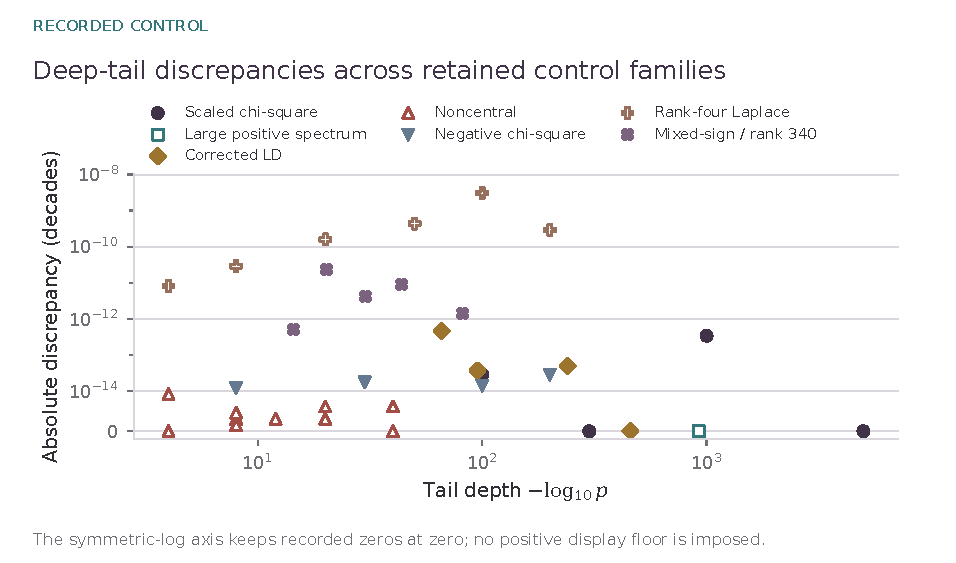
\includegraphics[width=\linewidth]{figures_production/figure_23_deep_tail_precision_envelope.pdf}
\caption{Retained log-probability discrepancies across positive, signed, mixed-sign, and noncentral control families. The symmetric-log vertical scale preserves exact stored zeros without a positive display floor. These are pointwise comparisons with the stated references, not uniform error bounds.}
\label{fig:deep-tail-precision-envelope}
\end{figure}

\subsection{Independent characteristic-function inversion near \texorpdfstring{\(10^{-16}\)}{1e-16}}

Closed-form controls are important, but they can hide numerical difficulties
that appear only for heterogeneous spectra.  An independent inversion test was
therefore run on four generalized chi-square laws near
\[
P(Q\ge q)\approx10^{-16}.
\]

The reference evaluates the original characteristic function directly through
the central Imhof inversion identity
\[
P(Q\ge q)
=
\frac12
+
\frac1\pi
\int_0^\infty
\frac{\sin\Theta(u)}{u\,R(u)}\,du,
\]
where, for distinct positive coefficients \(\lambda_j\) with multiplicities
\(h_j\),
\[
\Theta(u)
=
\frac12\sum_j h_j\arctan(\lambda_j u)
-
\frac12qu,
\qquad
R(u)
=
\prod_j
\left(1+\lambda_j^2u^2\right)^{h_j/4}.
\]
This route does not use exponential tilting, the COS expansion, spectral
packets, or the K-COS error controller.

The four spectra include balanced, skewed, dominant-spike, and higher-rank
cases.  Each reference integral was evaluated at two truncation limits.  The
omitted integral after the frequency cutoff \(T>0\) was bounded using
\[
\frac1\pi
\int_T^\infty\frac{du}{uR(u)}
\le
\frac{C}{\pi\nu}T^{-\nu},
\qquad
\nu=\frac12\sum_jh_j,
\qquad
C=\prod_j\lambda_j^{-h_j/2}.
\]

\begin{center}
\small
\begin{tabular}{@{}lrrrr@{}}
\toprule
spectrum & rank & \(|\Delta\log_{10}p|\) & relative difference & reference tail bound / \(p\)\\
\midrule
balanced & 80 & $6.52\times10^{-15}$ & $1.50\times10^{-14}$ & $6.84\times10^{-20}$\\
skewed & 80 & $4.13\times10^{-15}$ & $9.50\times10^{-15}$ & $4.44\times10^{-18}$\\
spiky & 80 & $5.19\times10^{-15}$ & $1.20\times10^{-14}$ & $7.00\times10^{-17}$\\
balanced & 120 & $2.88\times10^{-15}$ & $6.64\times10^{-15}$ & $4.19\times10^{-29}$\\
\bottomrule
\end{tabular}
\end{center}

The two inversion truncations agree to between approximately
\[
1.2\times10^{-21}
\quad\text{and}\quad
3.7\times10^{-17}
\]
decades across the four cases.  Thus the slow reference is numerically stable
at a scale well below the observed K-COS-versus-inversion difference.
Agreement between truncations is convergence evidence. The omitted-integral
bound alone does not enclose quadrature discretization or numerical rounding,
so this comparison is not assigned the directed-enclosure guarantee.

\begin{figure}[htbp]
\centering
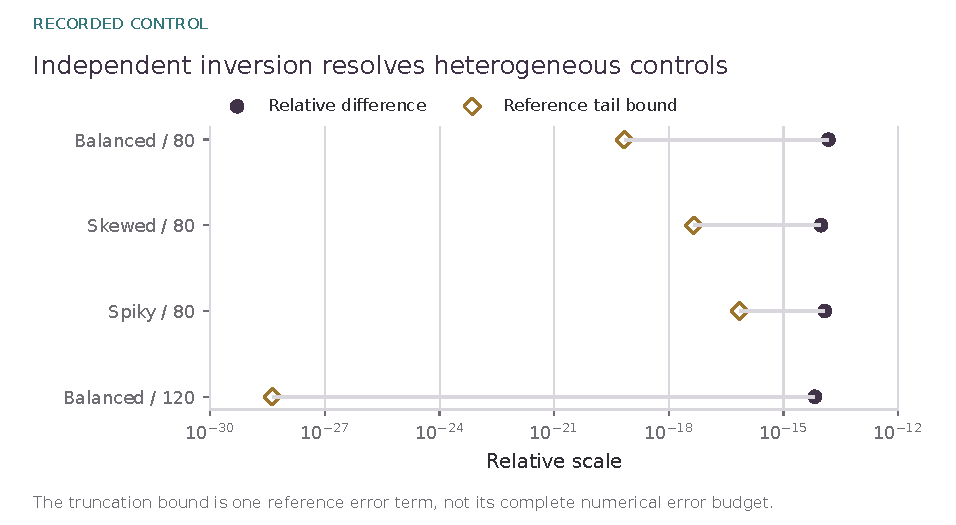
\includegraphics[width=\linewidth]{figures_production/figure_27_imhof_p1e16_validation.pdf}
\caption{Independent direct-inversion checks near $p=10^{-16}$ on four heterogeneous spectra. Circles show relative K-COS/reference differences and diamonds show the reference integral-tail bound. The latter is one error component, not a complete enclosure of all reference arithmetic.}
\label{fig:imhof-p1e16}
\end{figure}

This test is complementary to the exact scaled-chi-square controls.  It asks
whether the solver remains accurate when no single-gamma reduction is
available and when an algorithmically different inversion of the full
characteristic function is used as the reference.

These results have different evidentiary roles.  The scaled-chi-square,
finite-endpoint signed, Laplace signed, and noncentral cases provide analytic
controls.  The heterogeneous inversion battery, large-scale, strong-dependence, and
rank-340 mixed-sign cases test irregular spectra for which no single-gamma
closed form is available.  Together they test correctness against known distributions,
representation compression, and stability on the intended high-rank numerical
regime.  The low-rank Laplace example also records a deliberate certificate
failure boundary rather than conflating numerical agreement with certification.


\section{Signed and noncentral controls}
\paragraph{Exact finite-endpoint control.}
For
\[
Q=-0.02\,\chi^2_{80},
\]
the right tail is a lower chi-square tail with finite upper endpoint zero.  The
signed engine agrees with the exact distribution through
\[
\boxed{p=10^{-200}},
\]
with maximum observed log-probability error about $2.84\times10^{-14}$ decades
and certificates around $10^{-12}$.

\paragraph{Mixed-sign high-rank analytic-ledger control.}
A deterministic rank-340 multiscale spectrum with 180 positive and 160
negative coefficients was tested from approximately $10^{-14}$ to
\[
\boxed{p\approx10^{-81.891937}}.
\]
At the deepest point the packetized solver used 35 packets, $N=4096$, and
reported a relative certificate
\[
5.78\times10^{-9}.
\]
Its log-probability differed from the unpacketized full-spectrum signed solver
by about $1.42\times10^{-12}$ decades.  Independent exponential-tilt
importance sampling placed the discrepancy at about $1.41$ Monte Carlo
standard errors.

\paragraph{Retained low-rank limitation.}
For independent $Y_1,Y_2\sim\chi^2_2$, the quadratic form
\[
Q=0.07(Y_1-Y_2)
\]
is Laplace distributed with scale $0.14$, so for $q\ge0$,
\[
P(Q\ge q)=\frac12e^{-q/0.14}.
\]
The computed values agree with this exact law through $10^{-200}$ to roughly
$10^{-9}$ decades or better.  However, the implemented analytic COS-series
certificate rejects these low-rank mixed cases because the tilted
characteristic function decays only as $|t|^{-2}$.  The implementation reports
this as a certificate failure rather than silently accepting the numerical
value.

\begin{figure}[htbp]
\centering
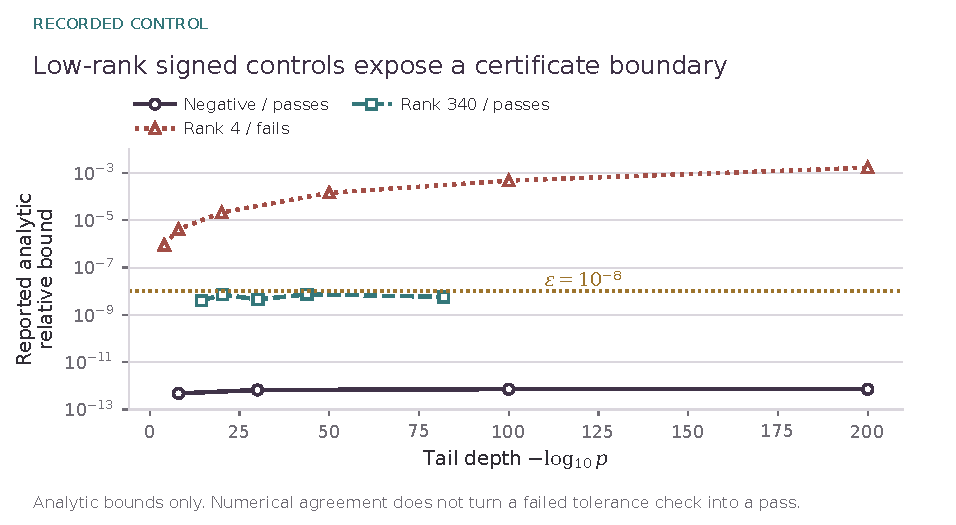
\includegraphics[width=\linewidth]{figures_production/figure_24_signed_certificate_boundary.pdf}
\caption{The negative finite-endpoint and rank-340 mixed-sign controls meet the requested analytic tolerance. The rank-four Laplace controls do not, despite close numerical agreement with their exact law. The horizontal line is the requested tolerance. These analytic-ledger results do not enclose floating-point roundoff.}
\label{fig:signed-certificate-boundary}
\end{figure}


\begin{figure}[htbp]
\centering
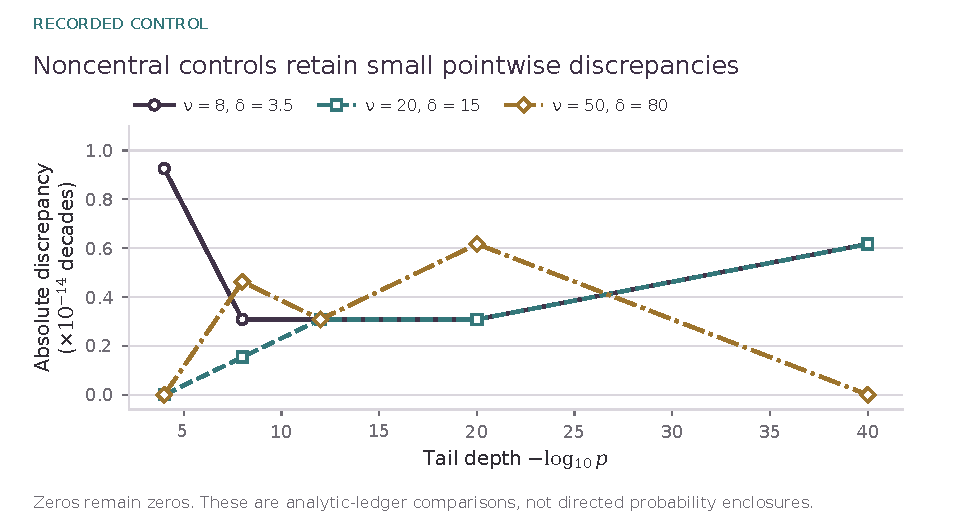
\includegraphics[width=\linewidth]{figures_production/figure_22_noncentral_controls.pdf}
\caption{Absolute log-probability discrepancies for three scaled noncentral chi-square families, labeled by degrees of freedom and noncentrality. Recorded zeros remain at zero. All analytic truncation checks pass, but this comparison is not a directed probability enclosure.}
\label{fig:noncentral-controls}
\end{figure}


\section{Rare-variant kernel case study}\label{sec:final-24}

The preceding sections establish operator identities and certified numerical
bounds.  This section tests the same machinery on the project's existing
rare-variant SKAT simulation layer, including explicit LD structure,
covariates, per-variant standardization, rare-variant weighting, and the
phenotype-space score statistic.

\subsection{Simulation provenance and implementation correction}

Two established genotype generators were used.

The first is a latent-Gaussian block-LD generator.  Within a genomic block,
alleles are obtained by thresholding correlated Gaussian latent variables at
variant-specific minor-allele frequencies.

The second is a copy-LD generator in which haplotype states persist along a
block with high probability and are occasionally redrawn. The simulator
must initialize its genotype accumulator to zero before adding haplotypes.
Allocating the accumulator with \verb|np.empty| and then applying
\verb|+=| would make the output depend on unspecified memory contents.
All copy-LD results reported here use explicit zero initialization. Results
from an uninitialized accumulator are excluded from the evidence record.

\subsection{Tested LD regimes}

Four deterministic scenarios were evaluated.

\begin{table}[htbp]
\centering
\caption{Synthetic rare-variant simulation scenarios.  Adjacent $r^2$ is
computed within the simulated LD blocks after variant standardization.}
\begin{tabular}{lrrrrr}
\toprule
scenario & $n$ & $m$ & rank & median adjacent $r^2$ & effective rank\\
\midrule
latent LD, moderate & 600 & 3000 & 596 & 0.0069 & 441.9\\
latent LD, strong & 600 & 3000 & 596 & 0.1140 & 240.3\\
copy LD, strong & 600 & 3000 & 596 & 0.8298 & 200.1\\
copy LD, large & 1000 & 5000 & 996 & 0.8179 & 353.0\\
\bottomrule
\end{tabular}
\end{table}

Effective rank here is the participation ratio
\[
r_{\rm eff}=\frac{(\sum_j\lambda_j)^2}{\sum_j\lambda_j^2}.
\]
It measures spectral concentration, not an integer count of nonzero directions.
The corresponding spectra therefore span a substantial range of concentration:
stronger LD reduces effective rank even when the nominal quadratic-form rank
remains close to the sample residual dimension.

\begin{figure}[htbp]
\centering
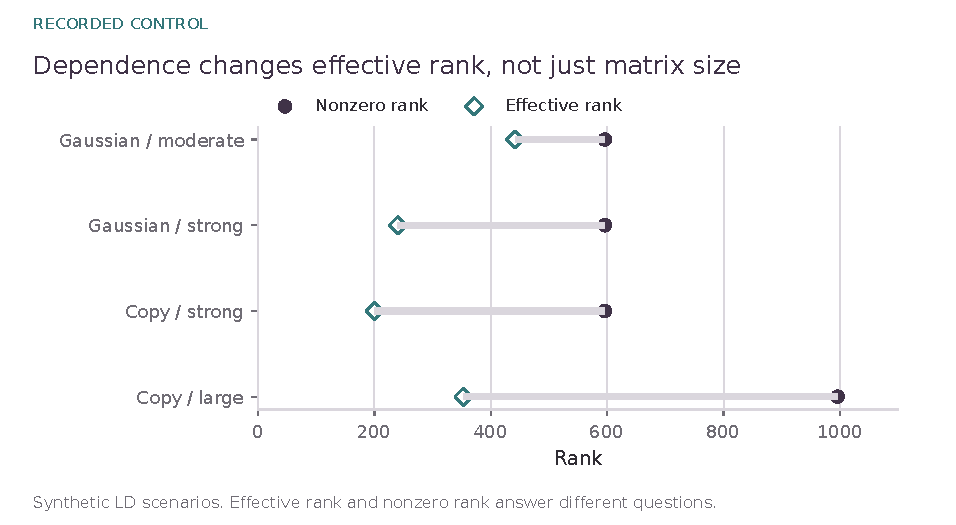
\includegraphics[width=\linewidth]{figures_production/figure_18_realistic_ld_effective_rank.pdf}
\caption{Nonzero and effective rank across four synthetic dependence scenarios. Connectors pair the two quantities for each scenario. Stronger dependence changes spectral concentration substantially even when nonzero rank is unchanged.}
\label{fig:realistic-ld-rank}
\end{figure}

\subsection{Streaming directly from raw genotype blocks}

The raw genotype matrix was streamed in resident variant blocks of widths
31, 127, and 509.  Within each block the implementation performs

\[
\begin{aligned}
G_b&\longrightarrow G_b-\bar G_b
     \longrightarrow \widetilde G_b,\\
\widetilde G_b&\longrightarrow M_X\widetilde G_b
     \longrightarrow A_b=M_X\widetilde G_bW_b^{1/2}
     \longrightarrow A_bA_b^\top,
\end{aligned}
\]

where $\widetilde G_b$ denotes the centered and scaled block. The full
weighted factor is never materialized.

Across all four LD scenarios and all three resident block sizes, the largest
relative discrepancy against the fully materialized kernel was

\[
\boxed{6.61\times10^{-16}}.
\]

\begin{figure}[htbp]
\centering
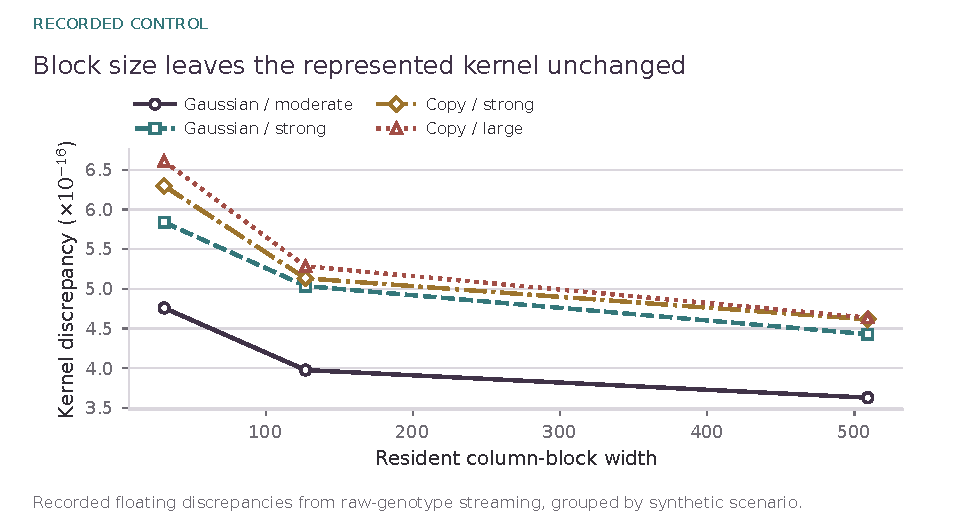
\includegraphics[width=\linewidth]{figures_production/figure_19_realistic_streaming_invariance.pdf}
\caption{Retained raw-genotype streaming discrepancies across synthetic dependence regimes and resident block widths. Marker shapes distinguish the scenarios in grayscale as well as color. The plotted differences are at floating-point summation scale.}
\label{fig:realistic-streaming}
\end{figure}

This test is stronger than applying the streamed identity to a precomputed
factor because the centering, variance scaling, covariate projection, and
rare-variant weights are all performed inside the block loop.

\subsection{Phenotype-space equivalence}

For each scenario, 100 Gaussian null residual draws were evaluated in three
ways. Under the standardized Gaussian null, write $e=M_Xz$ with
$z\sim N(0,I)$. Because $M_XA=A$, the statistic used here is
$Q=\frac12 z^\top Kz$, so its nonzero mixture coefficients are
$\frac12\lambda_j(K)$. The factor $\frac12$ belongs to this case-study
normalization, not to the general quadratic-form definition.

\begin{enumerate}
\item directly through the factor,
\[
Q=\frac12\|A^\top e\|_2^2.
\]
\item through the sample kernel,
\[
Q=\frac12 e^\top Ke.
\]
\item through the eigencoordinates of $K$.
\end{enumerate}

The worst relative discrepancy across all draws and all scenarios was

\[
\boxed{8.32\times10^{-16}}.
\]

Thus the simulated phenotype path, the streamed kernel, and the generalized
$\chi^2$ spectral representation agree to floating-point precision.

\subsection{Deep tails on simulated LD spectra}

For every scenario, tail queries were generated at tilt fractions
0.90, 0.97, and 0.99 of the positive singularity.  K-COS was compared with a
higher-resolution full-spectrum tilted reference.

The large corrected copy-LD case was then pushed further, to fractions
0.995, 0.997, 0.999, and 0.9995.  The deepest tested reference value was

\[
\boxed{\log_{10}p=-457.973916}.
\]

At that point the displayed K-COS and high-resolution full-spectrum values
were identical.  Across the complete realistic-LD battery, the largest
absolute discrepancy was

\[
\boxed{3.21\times10^{-12}\ \text{decades}}.
\]

\begin{figure}[htbp]
\centering
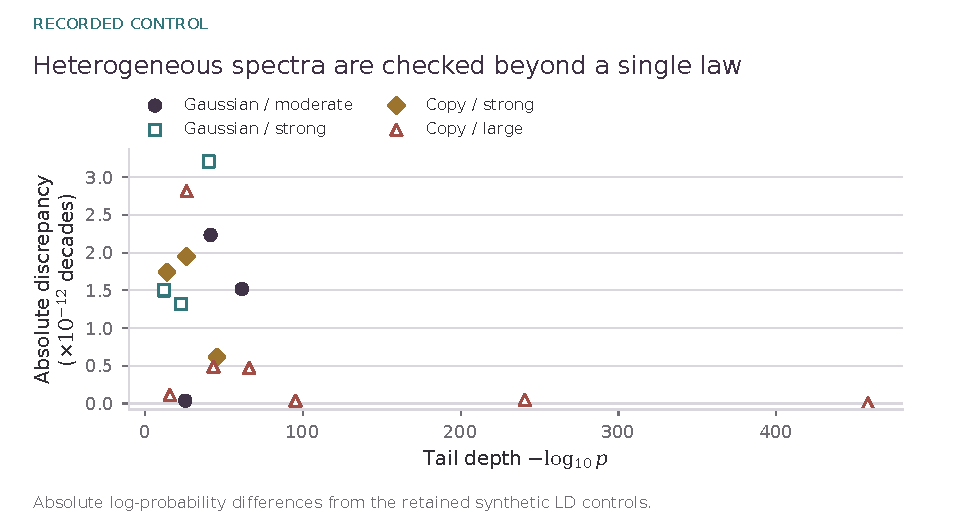
\includegraphics[width=\linewidth]{figures_production/figure_20_realistic_deep_tail_accuracy.pdf}
\caption{Absolute differences between K-COS and refined full-spectrum tilted references on the synthetic dependence scenarios. The corrected large copy-LD controls extend through approximately $10^{-458}$. Zeros are plotted at zero rather than assigned an artificial positive floor.}
\label{fig:realistic-deep-tail}
\end{figure}

For the $n=1000$, $m=5000$ corrected copy-LD spectrum, selected results are

\begin{center}
\begin{tabular}{rrrr}
\toprule
tilt fraction & $\log_{10}p$ & COS modes $N$ & absolute error (decades)\\
\midrule
0.9950 & -65.950669 & 2048 & $4.69\times10^{-13}$\\
0.9970 & -95.305034 & 2048 & $3.70\times10^{-14}$\\
0.9990 & -240.602047 & 8192 & $4.94\times10^{-14}$\\
0.9995 & -457.973916 & 16384 & below stored reference resolution\\
\bottomrule
\end{tabular}
\end{center}

\subsection{Interpretation and boundary}

This simulation block does not add a new algebraic theorem.  It supplies a
more demanding validation layer for the theorem chain already proved.
Specifically, it shows that the exact streaming identities and the K-COS
deep-tail machinery remain numerically stable under substantially different
rare-variant LD structures and through the complete raw-genotype preprocessing
path.

The evidence remains synthetic.  These generators do not reproduce every
population-genetic feature of a sequencing cohort, and this block is not an
external-cohort replication. It addresses the Gaussian linear-model null.
Finite-sample Bernoulli or logistic calibration remains a separate statistical
problem.



\section{Spectral-packet experiments}
These tables and figures report the retained packet-planner experiments.
Their analytic error bounds exclude floating-point roundoff. They measure a
different numerical path from the directed positive backend, and are not
reinterpreted as directed probability enclosures or new performance runs.

\subsection{Exactly solvable chi-square stress test}

To isolate the effect of exponential tilting, we first used
\[
Q=0.02\chi^2_{80},
\]
whose survival probabilities are available directly from the chi-square distribution. Table \ref{tab:chi} compares a global COS calculation with query-centered tilted COS.

\begin{table}[htbp]
\centering
\caption{Relative error in an exactly solvable chi-square family.}
\label{tab:chi}
\begin{tabular}{rrrr}
\toprule
Target tail $p$ & $N$ & Global COS rel. error & Tilted COS rel. error\\
\midrule
$10^{-6}$  & 64  & $3.56\times10^{-8}$ & $2.71\times10^{-14}$\\
$10^{-10}$ & 64  & $1.64\times10^{-4}$ & $6.59\times10^{-15}$\\
$10^{-10}$ & 128 & $2.03\times10^{-6}$ & $9.05\times10^{-15}$\\
$10^{-14}$ & 64  & $1.43$              & $3.53\times10^{-14}$\\
$10^{-14}$ & 128 & $6.15\times10^{-2}$ & $3.87\times10^{-14}$\\
\bottomrule
\end{tabular}
\end{table}

The test demonstrates the numerical motivation for tilting: evaluating a small tail directly under the shifted law is substantially more stable than reconstructing a global CDF and subtracting from one. This observation is not a novelty claim for exponential tilting itself.

\subsection{Genotype-derived spectra}

The second experiment used the existing Komorebi SKAT benchmark generator. Synthetic genotype matrices were centered and scaled, then residualized against three covariates. The kernel weights were $w_j=(1-\mathrm{MAF}_j)^{24}$, where MAF denotes minor-allele frequency. The factor used column scales $\sqrt{w_j}$. Its positive quadratic-form spectrum was
\[
\lambda=\tfrac12\operatorname{eig}(AA^{\mathsf T}).
\]
Three independent $n=400$, $m=1200$ genotype sets yielded numerical rank $397$. Four upper-tail queries per spectrum were generated by choosing saddlepoint locations at fractions $0.70,0.80,0.85,0.90$ of the transform singularity. The comparison reference used exact-spectrum tilted COS with $N=2048$ and a large support parameter $L=20$. The adaptive method was asked for a relative analytic tolerance of $10^{-8}$.

Across the twelve queries:
\begin{itemize}
\item every requested $10^{-8}$ analytic certificate passed.
\item the worst observed relative error was $6.148608\times10^{-11}$.
\item the largest returned analytic relative bound was $7.917203\times10^{-9}$.
\item the planner selected $N\in\{64,128\}$, $L\in\{10,11,12,13\}$, and 11--16 packets.
\end{itemize}

Figure \ref{fig:coverage} plots the observed errors against the returned analytic bounds. Every point lies above the equality line because the vertical coordinate is the bound.

\begin{figure}[htbp]
\centering
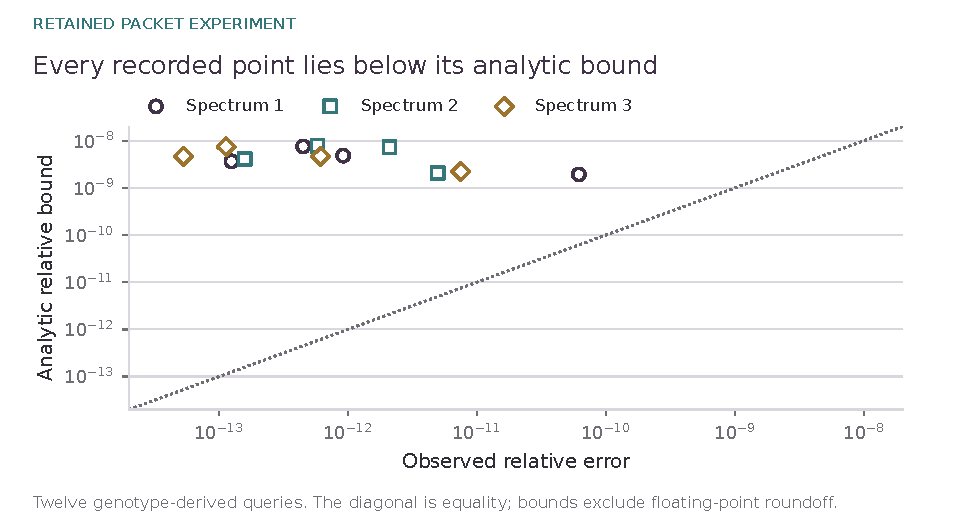
\includegraphics[width=\linewidth]{figures_production/certificate_coverage.pdf}
\caption{Twelve retained genotype-derived tail queries, redrawn from the recovered source table. The vertical coordinate is the analytic relative bound and the horizontal coordinate is observed relative error. Every point lies above equality. Marker shape identifies the source spectrum.}
\label{fig:coverage}
\end{figure}

\subsection{Tolerance ladder}

At a reference tail probability near $8.99\times10^{-15}$, the same engine was requested to meet three tolerances. Table \ref{tab:ladder} shows how the representation refined automatically.

\begin{table}[htbp]
\centering
\caption{Adaptive refinement at an extreme-tail query.}
\label{tab:ladder}
\begin{tabular}{rrrrrr}
\toprule
Requested $\tau$ & $N$ & $L$ & Packets & Analytic bound & Observed error\\
\midrule
$10^{-6}$  & 128 & 10 & 10 & $3.56\times10^{-7}$  & $3.63\times10^{-12}$\\
$10^{-8}$  & 128 & 12 & 15 & $4.87\times10^{-9}$  & $9.14\times10^{-13}$\\
$10^{-10}$ & 256 & 14 & 24 & $8.21\times10^{-11}$ & $5.65\times10^{-14}$\\
\bottomrule
\end{tabular}
\end{table}

\begin{figure}[htbp]
\centering
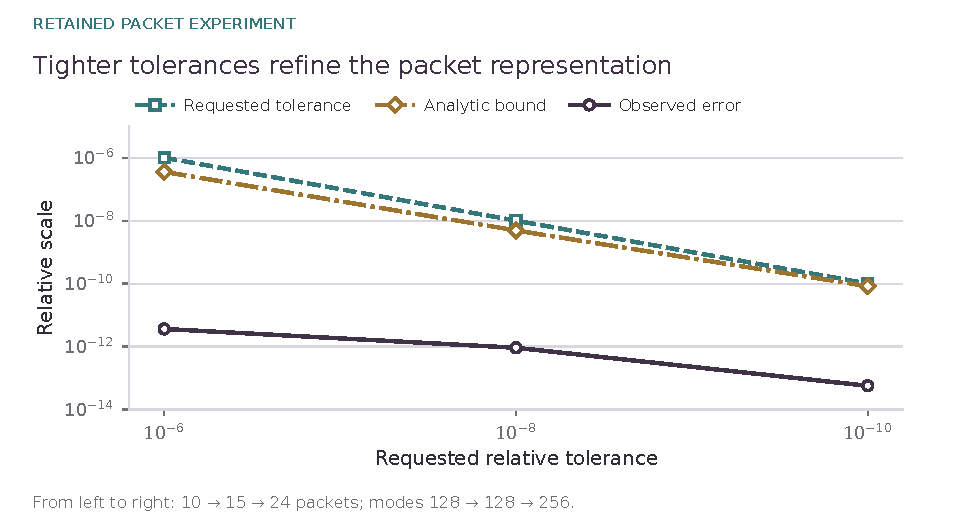
\includegraphics[width=\linewidth]{figures_production/tolerance_ladder.pdf}
\caption{One extreme-tail query evaluated under three requested tolerances. Increasing the accuracy request refines the packet representation and, at the tightest setting, the mode count. The returned analytic bound remains above observed error and below the requested tolerance.}
\label{fig:ladder}
\end{figure}

\subsection{Prototype runtime scaling}

Table \ref{tab:runtime} reports median CPU timings from the Python prototype. ``Adaptive total'' includes planning and analytic error checks. ``Compiled evaluation'' measures reuse of an already compiled spectral passport at the selected grid.

\begin{table}[htbp]
\centering
\caption{Prototype runtime scaling on genotype-derived spectra.}
\label{tab:runtime}
\begin{tabular}{rrrrrr}
\toprule
Rank & Packets & Exact tilted & Adaptive total & Compiled eval. & Compiled speedup\\
\midrule
397  & 13 & 6.66 ms & 10.45 ms & 0.549 ms & $12.1\times$\\
797  & 16 & 13.32 ms & 11.49 ms & 0.604 ms & $22.0\times$\\
1197 & 17 & 21.52 ms & 11.24 ms & 0.651 ms & $33.1\times$\\
\bottomrule
\end{tabular}
\end{table}

\begin{figure}[htbp]
\centering
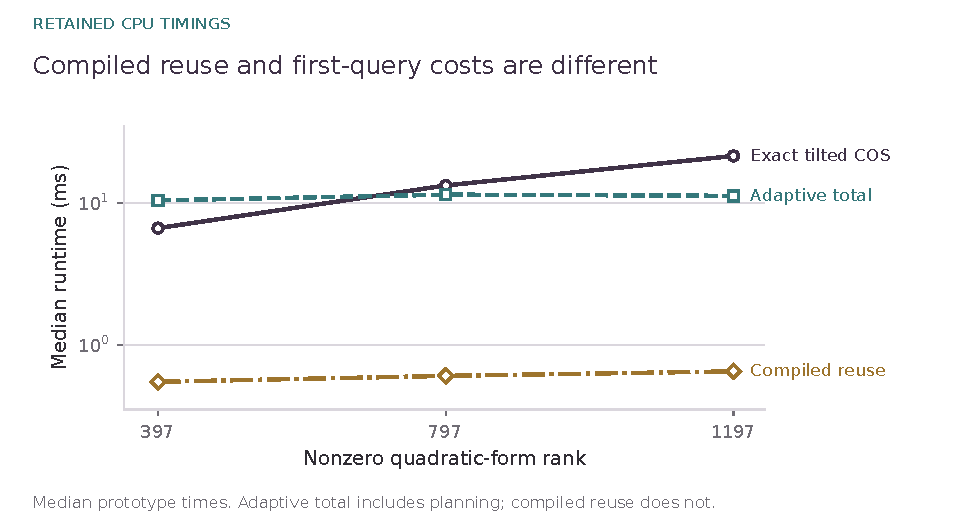
\includegraphics[width=\linewidth]{figures_production/runtime_scaling.pdf}
\caption{Retained median CPU timings for exact tilted COS, the adaptive calculation including planning, and reuse of a compiled spectral representation. The logarithmic vertical scale keeps the much smaller reuse cost visible. First-query and reuse costs are not interchangeable.}
\label{fig:runtime}
\end{figure}

Planning matters. The first adaptive query is slower at rank 397 and faster at rank 797 in this prototype. Compiled reuse measures a different cost. These timings establish no universal speedup.



\section{Numerical verification}\label{sec:final-28}

\begin{table}[htbp]
\centering
\caption{Stored-run identifiers and actual block counts.}
\begin{tabular}{lrrr}
\toprule
partition & blocks & Gram relative error & action relative error\\
\midrule
coarse 4 & 4 & \(2.91\times10^{-16}\) & \(5.99\times10^{-16}\)\\
fine 64 & 32 & \(3.39\times10^{-16}\) & \(6.00\times10^{-16}\)\\
irregular & 9 & \(3.34\times10^{-16}\) & \(5.87\times10^{-16}\)\\
singleton-front & 21 & \(2.43\times10^{-16}\) & \(5.82\times10^{-16}\)\\
permuted, block 73 & 29 & \(3.52\times10^{-16}\) & \(5.89\times10^{-16}\)\\
\bottomrule
\end{tabular}
\end{table}

Hierarchical refinement gave relative discrepancy $3.17\times10^{-16}$.
For $H=L^\top L$ with block-bidiagonal $L$, the smallest eigenvalue was
approximately $2.86$ and the largest norm outside the exact light cone
was zero. The QR-core singular-spectrum discrepancy was
$5.89\times10^{-16}$ in relative $\ell_2$ norm. These are finite controls,
not universal floating-point error bounds.




\chapter{Composition, scope, and contribution}\label{ch:synthesis}
\chapterlead{The useful synthesis is not that every decomposition commutes with every
other. It is that each layer preserves a specified object or exposes a
specified error. The final calculation is justified only when those objects
and bounds agree at their interfaces. This chapter states the exact
composition result, locates the contribution among established methods, and
makes the remaining implementation boundaries explicit.}
\section{Method synthesis: composable decompositions}\label{sec:final-29}

The solver is organized around four independent decomposition axes:
\[
\boxed{
\mathcal D
=
\mathcal D_{\rm storage}
\circ
\mathcal D_{\rm phase}
\circ
\mathcal D_{\rm rank}
\circ
\mathcal D_{\rm spectrum}.
}
\]
This display describes the pipeline schematically, not four endomorphisms
proved to commute pairwise.  The precise commutation theorem below is for
exact storage refinement and a fixed structural phase partition.  Full range
capture or residual completion preserves the nonzero spectrum exactly. A
truncated packet representation instead preserves the requested tail within
its explicit analytic error bound.

They answer different questions.  Storage decomposition controls what is
resident.  Phase decomposition controls where information can propagate.
Rank decomposition controls how many directions must be retained.  Spectral
packetization controls the cost of the final deep-tail transform.  The central
structural fact is that these representations can be changed independently
without changing the exact operator when their respective invariance
conditions are satisfied.

\subsection{Storage-phase commutation}

Fix a structural phase partition
\[
\{1,\ldots,m\}=\mathcal P_1\sqcup\cdots\sqcup\mathcal P_H
\]
and let each phase be subdivided into arbitrary storage blocks
\[
\mathcal P_h
=
J_{h1}\sqcup\cdots\sqcup J_{hB_h}.
\]
Let $S$ denote this physical storage subdivision.  The phase projectors
$P_h$ are defined by the structural phases, not by $S$.

\begin{theorem}[Storage-phase commutation theorem]\label{claim:final-29-1}
Let
\[
A=M_XGW^{1/2},
\qquad H=A^\top A,
\]
and let $S$ and $S'$ be any two exact storage refinements that respect the
same structural phase partition.  Then:
\begin{enumerate}[label=(\roman*)]
\item the exact operator $H$ is identical under $S$ and $S'$.
\item every phase coupling $P_hHP_g$ is identical under $S$ and $S'$.
\item the exact phase graph and every $k$-step polyphase light cone are
identical under $S$ and $S'$.
\item any exact matrix-free Krylov method applied through streamed products
produces the same Krylov subspaces in exact arithmetic under $S$ and $S'$.
\end{enumerate}
\end{theorem}

\begin{proof}
Storage refinement changes only the order and grouping of finite sums.
By partition refinement invariance, the streamed products reconstruct the
same $A$, $A^\top$, and therefore the same $H=A^\top A$.  Since each
$P_h$ is fixed by the structural phase partition, every block
$P_hHP_g$ is unchanged.  The phase graph is defined only by these blocks, so
its path structure and light cones are unchanged.  Finally, an exact
matrix-free Krylov method depends only on repeated applications of the same
operator to the same starting block. Hence its generated subspaces are
identical.
\end{proof}

\begin{corollary}[Adaptive resident-block scheduler]\label{claim:final-29-2}
An implementation may change resident block size at runtime, including
recursive splits after an allocation failure, without changing the exact
phase graph or the exact Krylov subspaces. All required storage blocks must
be processed exactly, with the operator and starting block held fixed.
\end{corollary}

This separates \emph{mathematical locality} from \emph{physical storage
granularity}.  A phase may remain fixed as an LD window or annotation class
while its physical representation is subdivided according to free GPU
memory, scalar precision, transfer granularity, or stream count.

\subsection{Frontier-to-I/O theorem}

\begin{theorem}[Exact frontier-to-I/O reduction]\label{claim:final-29-3}
Suppose a validated exact phase graph of the fixed operator $H=A^\top A$
is already supplied and the initial Krylov block is supported on a phase set
$F_0$.  Keep covariate projections, weights, and structural phase metadata
fixed, and assume all factor-action blocks required for the retained phase
operator are available.  At depth $k$, let $F_k$ be the graph
$k$-neighborhood of $F_0$.  Then no storage block lying wholly in a phase
outside $F_k$ can affect the $k$-step Krylov vector.  Such a block need not be
loaded when evaluating the requested power through the restricted factor
$A_{F_k}$.  Storage blocks mixing active and inactive phases require a
separate refinement before this omission is valid.
\end{theorem}

\begin{proof}
For every phase $h\notin F_k$ and every starting phase $g\in F_0$, the
polyphase light-cone theorem gives $P_hH^kP_g=0$.  Storage-phase commutation
allows each active phase operator to be evaluated through arbitrary exact
storage blocks.  Every path of length at most $k$ beginning in $F_0$ stays in $F_k$.
Let $J_F$ be the coordinate inclusion from the retained coordinates
$F=F_k$ into the full variant space. Thus $P_F=J_FJ_F^\top$ and
$A_F=AJ_F$. The compressed operator and its ambient embedding satisfy
\[
H_F=J_F^\top HJ_F=A_F^\top A_F,
\qquad P_FHP_F=J_FH_FJ_F^\top.
\]
These identities distinguish the compressed matrix from the larger ambient
matrix. Since every path of length at most $k$ from $F_0$ stays in $F$,
\[
H^kX=J_F H_F^k J_F^\top X.
\]
This includes the zero output outside $F$. Blocks wholly outside the retained
phase set may therefore be omitted from the restricted factor evaluation.
\end{proof}

The theorem turns an algebraic support statement into an execution law:
\[
\boxed{
\text{Krylov depth}
\longrightarrow
\text{reachable phases}
\longrightarrow
\text{storage blocks that must be transferred}.
}
\]
Discovery or verification of the phase graph may itself require all inputs.
The theorem does not claim minimum total I/O, omission of mixed-phase blocks,
or correctness for an unverified approximate graph.  The scheduler is constrained
by the exact operator graph rather than solely by available memory.

\subsection{Full method stack}

The representation pipeline may therefore be written as
\[
\boxed{\begin{aligned}
A
&\longrightarrow \text{resident storage blocks}\\
&\longrightarrow \text{structural phase frontier}\\
&\longrightarrow \text{phase-local Krylov/range core}\\
&\longrightarrow \text{residual moment certificate or exact completion}\\
&\longrightarrow \text{spectrum or verified spectral enclosure}.
\end{aligned}}
\]

From that point the implementation has two numerical paths. Centered packets
lead to an analytic error ledger evaluated in floating point. Direct evaluation
of the supplied positive spectrum leads to a directed probability enclosure.
The second path does not yet certify packet construction or packet arithmetic.

Three invariances make the stack composable:
\begin{enumerate}
\item storage refinement does not change the represented operator.
\item structural phase scheduling does not depend on physical block size.
\item once the spectrum or a certified spectral enclosure is obtained, the
      tail engine is independent of the application that produced it.
\end{enumerate}

The resulting method can be aggressive during basis discovery and still return
to exactness.  Approximate phase pruning is controlled by query and operator
budgets. Unresolved range structure is measured by trace, square-trace, and
spectral-cap invariants. And when the remaining rank is small, streamed
residual completion restores the exact nonzero spectrum before the final tail
evaluation.

\subsection{Method summary}

The resolved synthesis is
\[
\boxed{\begin{aligned}
&\text{exact streamed factor actions}
+\text{ structural light cones}
+\text{ certified pruning}\\
&+\text{ phase-local rank}
+\text{ residual moment certificates}
+\text{ exact residual completion}\\
&+\text{ spectral packets}
+\text{ log-domain extreme-tail evaluation}.
\end{aligned}}
\]

The central design principle is separation of representation from semantics:
changing how an operator is stored, scheduled, compressed, or evaluated must
not silently change the mathematical quadratic form.  Each approximation
layer therefore either carries an explicit certificate or terminates in an
exact completion step.



\section{Prior work and the contribution boundary}\label{sec:prior-work}
Characteristic-function methods for quadratic forms substantially predate
this engine.  Imhof's 1961 paper is a foundational historical comparator
\cite{Imhof1961}.  Davies' Algorithm AS~155 treats linear combinations of
noncentral chi-square variables with signed coefficients and an optional
Gaussian term, using characteristic-function inversion and explicit
truncation/integration controls \cite{Davies1980}.  Its documented difficult
low-degree cases are relevant to the retained low-rank limitations here.

The Fourier-cosine representation and the use of characteristic-function
values for cosine coefficients are due to Fang and Oosterlee
\cite{FangOosterlee2008}.  Their formulation distinguishes finite-domain
coefficients from the full characteristic-function coefficients used to
approximate them.  The support/folding argument above supplies the particular
positive-law alias bound needed here. A general COS accuracy theorem is not
inherited without checking its hypotheses.

The choice of truncation range is studied by Junike and Pankrashkin
\cite{JunikePankrashkin2022}, and explicit mode-count bounds under stated
regularity assumptions by Junike \cite{Junike2024}. Junike and Stier develop
a damped COS framework for distributional quantities and related integrals
\cite{JunikeStier2025}. These are relevant predecessors to the support,
mode, and reweighting layers. The bounds proved here are specialized to the
quadratic-form transform and must be justified under their own hypotheses.

No novelty is claimed for Gaussian spectral reduction, exponential tilting,
saddlepoint centering, Fourier-cosine inversion, Weyl bounds, QR updates, or
out-of-core multiplication themselves.  The proposed contribution is their
explicit integration with independently adjustable storage, structural,
range-residual, and query-specific centered spectral representations.  The
packet compiler in Chapter~\ref{ch:packets} is a concrete mechanism: its
local CGF remainder is propagated to the requested tail functional and
refined jointly with support and mode errors.  The finite refinement theorem
is an existence theorem, not a complexity guarantee or proof of planner
optimality.

The source-attribution record supports the listed COS and Davies formulas
and the Imhof bibliographic entry. It is not an exhaustive priority search.
The independent Imhof-style inversion checks support accuracy on the tested
heterogeneous spectra. They do not establish a universal runtime advantage
over a mature Davies implementation.


\section{Guarantee levels and scope}\label{sec:final-31}

The framework contains several different evidence levels.  They are kept
separate because a proved algebraic identity, a finite numerical validation,
and a directed-rounding probability enclosure are different kinds of claims.

\begin{center}
\small
\begin{tabular}{@{}P{0.30\linewidth}P{0.20\linewidth}P{0.41\linewidth}@{}}
\toprule
Statement & Status & Meaning\\
\midrule
Block factor and streamed-action identities &
proved &
Exact finite-dimensional matrix identities. Storage blocking introduces no
mathematical approximation.\\

Storage-phase commutation and exact light cones &
proved &
Physical block refinement does not change the structural phase graph. Phases
outside the exact finite-depth frontier contribute zero.\\

Approximate light-cone and pruning certificates &
proved + tested &
Weak discarded couplings carry explicit finite-depth transfer and
operator-norm budgets.\\

Range residual and exact completion &
proved + tested &
The unresolved factor is measured directly. Small residual rank can be
completed exactly.\\

Positive exact-spectrum tail enclosure &
directed rounding + proved remainders &
For rank \(>2\), the finite transform is enclosed numerically and enlarged by
proved support/alias and infinite-mode bounds.\\

Accuracy-driven positive tail solver &
certified / fail-closed &
A result is accepted only after
\(p_+/p_- - 1\le\varepsilon_{\rm requested}\) is proved.\\

Positive noncentral engine &
exact reduction + tested tail solver &
The Gaussian form is reduced to a deterministic shift plus positive
noncentral chi-square components.\\

Signed / indefinite engine &
proved reduction + analytic-ledger tests &
High-rank and finite-endpoint cases passed analytic error checks. Low-rank mixed-sign forms
remain limited by slow Fourier decay of the present COS certificate.\\

Binary64 factor to rigorous spectrum &
implemented at moderate dimension &
Candidate eigensystems are post-certified by directed-rounding orthogonality
and reconstruction bounds, then propagated monotonically into the tail.  The
remaining issue is scalable streamed/subspace verification rather than the
basic correctness theorem.\\
\bottomrule
\end{tabular}
\end{center}

Four implementation boundaries remain material:

\begin{enumerate}
\item The verified matrix-to-spectrum bridge is dense. Its streamed range-core
and residual-completion counterparts require verified linear algebra.
\item Packet construction and evaluation are not implemented with directed
rounding. Their analytic ledgers remain distinct from numerical enclosures.
\item The mixed-sign low-rank certificate is conservative. Signed and noncentral
numerical paths do not inherit the positive backend's directed guarantee.
\item Native GPU execution and hardware transfer/compute crossover measurements
are outside the supplied Python implementation and recorded benchmarks.
\end{enumerate}

These are boundaries of the implementation, not hidden assumptions in the
certified positive matrix-to-tail result at moderate dimension.



\section{Conclusion}\label{sec:final-32}

The quadratic-form problem can be separated into representation, structure,
spectral recovery, and tail evaluation.

At the representation level, factors can be streamed in blocks without
changing the operator.  At the structural level, phase graphs constrain
finite-depth propagation and allow certified scheduling.  At the spectral
level, unresolved range structure is measured rather than guessed and can be
completed exactly when its rank becomes small.  At the probability level,
exponential tilting and spectral packets make extreme tails computationally
tractable, while directed-rounding interval arithmetic and analytic remainder
bounds turn the positive exact-spectrum calculation into an explicit
probability enclosure.

The resulting numerical contract is deliberately stronger than
``approximately evaluate a small probability.''  For the rigorous positive
backend, the user supplies an accuracy requirement.  Internal resolution is
refined until that requirement is proved, or the solver returns an
uncertified interval rather than claiming success.

The deepest retained exact control reaches
\[
p\approx10^{-5000}.
\]
At that point the recorded accuracy-driven run reported relative multiplicative
uncertainty below \(10^{-18}\).  This establishes that extreme-tail depth by
itself is not the limiting numerical variable. The meaningful limit is whether
the complete error ledger can be made smaller than the requested tolerance.

The matrix-to-spectrum bridge closes that upstream correctness gap for
moderate binary64 factors by post-certifying an otherwise untrusted candidate
eigensystem.  Further numerical guarantees require scalable
representation and a directed implementation of packet arithmetic: carry the same enclosure through streamed range cores and
residual completion without forming a full dense eigenbasis, while extending
the fail-closed accuracy contract to difficult low-rank mixed-sign forms.





\appendix
\bookmarksetup{startatroot}
\chapter{Visual studies}\label{app:atlas}
\begingroup\small
These studies follow declared finite examples from an exact factor to a probability enclosure. Their Python sources and inputs accompany the volume. They are explanatory calculations, not additional production benchmarks.

{\displayface\fontsize{27}{30}\selectfont\color{ink}From a factor to a justified tail\par}
\vspace{3pt}
\begin{center}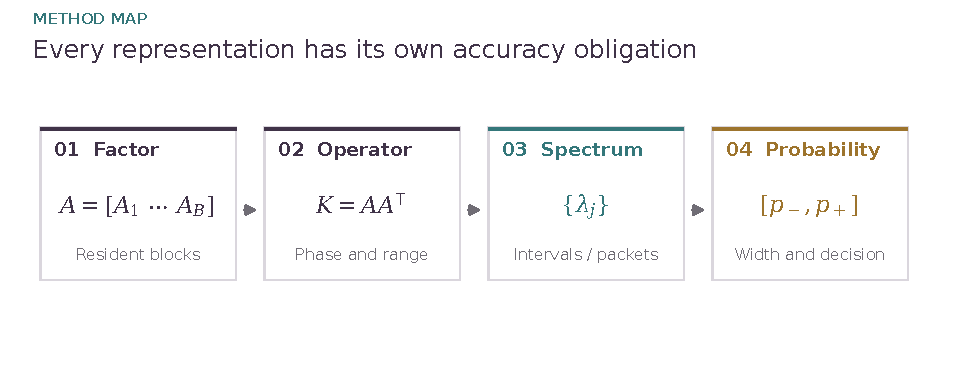
\includegraphics[width=\linewidth]{figures_production/00_pipeline.pdf}\end{center}
The four layers answer different questions: what must reside in memory, what can propagate, what range remains unresolved, and how the tail calculation meets its accuracy contract.

Integer controls check block identities and phase zeros. Floating calculations illustrate compression and analytic bounds. A finite positive sum supplies an independent deep-tail control. The main chapters supply the proofs, Appendix~\ref{app:lean} identifies formal coverage, and the final study separates algebraic, analytic, and numerical evidence.

\studyresult{Preserve exact identities where possible. Expose every approximation at the point where it enters.}
\vfill{\footnotesize\color{navy}\textbf{Reading connection.} Chapter~\ref{ch:synthesis}.}
\clearpage
\atlasheading{01}{Factor and law}{A spectrum is the distributional interface}
\vspace{3pt}
\begin{center}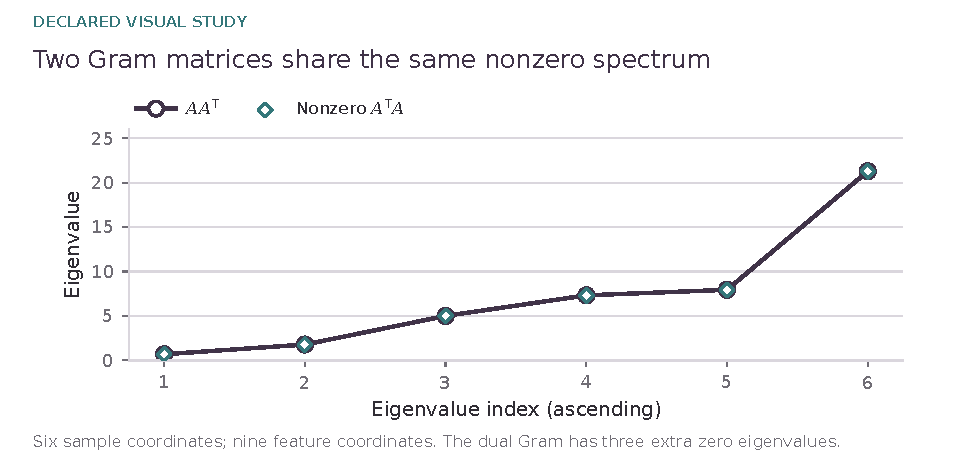
\includegraphics[width=\linewidth]{figures_production/01_factor_spectrum.pdf}\end{center}
{\small\color{navy}Two numerically evaluated nonzero Gram spectra for the declared integer factor. Their matching points use distinct markers.}

\[X=\Sigma^{1/2}Z,\quad Z\sim N(0,I),\quad H=\Sigma^{1/2}M\Sigma^{1/2}.\]
\[X^{\mathsf T}MX\overset d=\sum_{j=1}^{r}\lambda_jZ_j^2,\qquad \lambda_j\in\operatorname{spec}(H)\setminus\{0\}.\]
For a central Gaussian vector with covariance $\Sigma\succeq0$ and symmetric $M$, the quadratic form becomes a weighted sum of independent standard-normal squares after whitening and orthogonal diagonalization. The operator may originate in a kernel, a signal model, or another symmetric construction. Once its spectrum has been correctly obtained, the tail layer sees those coefficients.

The nonzero eigenvalues of the two Gram matrices coincide. The small integer factor in this guide has six sample coordinates and nine feature coordinates. One Gram matrix therefore has six eigenvalues. The other has the same six nonzero eigenvalues plus three zeros. The figure compares their floating evaluations.

Positive coefficients give support on the nonnegative half-line. Signed coefficients define a different support problem. The exact reduction extends to symmetric indefinite forms, while the positive-support interval backend developed later has narrower hypotheses.

\studyresult{Representation equivalence is exact mathematics. Certifying computed eigenvalues is a further numerical obligation.}
\vfill{\footnotesize\color{navy}\textbf{Reading connection.} Chapter~\ref{ch:gaussian}.}
\clearpage
\atlasheading{02}{Storage partition}{Column blocks add their Gram operators exactly}
\vspace{3pt}
\begin{center}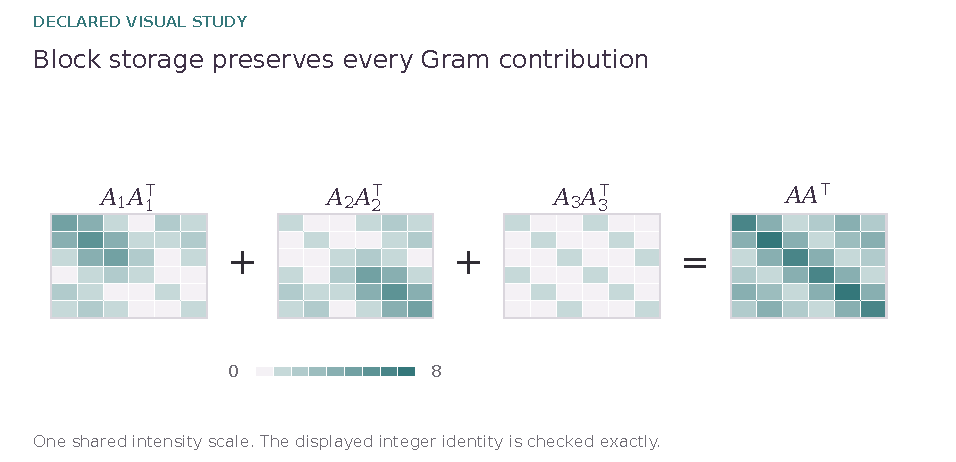
\includegraphics[width=\linewidth]{figures_production/02_block_gram.pdf}\end{center}
{\small\color{navy}All block Gram contributions use the same color scale. Their exact sum is the full sample kernel.}

\[A=[A_1\ \cdots\ A_B],\qquad AA^{\mathsf T}=\sum_{b=1}^B A_bA_b^{\mathsf T}.\]
\[KV=\sum_b A_b(A_b^{\mathsf T}V),\qquad A_b\in\mathbb R^{n\times c_b},\quad V\in\mathbb R^{n\times s}.\]
Partition a factor by columns and keep every block. Horizontal concatenation turns the sample-space Gram matrix into a sum of block Gram matrices. Changing the block widths or the order in which blocks are read preserves the represented operator.

The figure splits the declared $6\times9$ integer factor into three blocks of width three. Every matrix entry in the displayed identity is an integer, and the regeneration script checks equality exactly. Block storage introduces no statistical approximation.

A streamed action need not store each block kernel. It first multiplies by the block transpose, then by the block itself, and accumulates the sample-space result. The dimensions explain why the operator can remain exact even when the whole factor cannot reside at once.

\studyresult{Execution partitions determine residence and I/O. Keeping all blocks preserves the operator.}
\vfill{\footnotesize\color{navy}\textbf{Reading connection.} Chapter~\ref{ch:streaming}.}
\clearpage
\atlasheading{03}{Algebraic sizing}{Memory depends on the resident width}
\vspace{3pt}
\begin{center}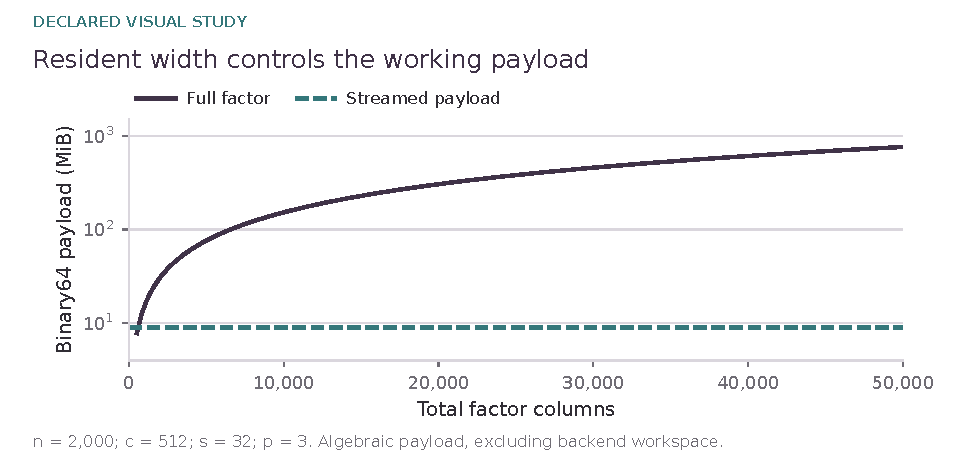
\includegraphics[width=\linewidth]{figures_production/03_memory.pdf}\end{center}
{\small\color{navy}An explicitly counted binary64 payload with fixed resident width. Total-factor storage grows linearly in $m$.}

\[\text{working storage}=O(nc+ns+cs+np).\]
\[\text{illustrated payload}=8\,(nc+2ns+cs+np)\ \text{bytes}.\]
A full factor holds $nm$ scalar entries. A streamed action with resident width $c$ and block-vector width $s$ keeps a factor block and a small number of action buffers. Residualization against a covariate basis of rank $p$ adds $np$ entries. At fixed $c,s,p$, this algebraic working set does not grow with total column count $m$.

The sizing curve is an illustration, not a measured memory profile. It uses $n=2000$, $c=512$, $s=32$, $p=3$, and binary64 entries. The plotted streamed payload counts one resident factor, two sample buffers, one block intermediate, and the covariate basis.

Backend workspace, I/O buffers, saved outputs, and spectral-solver storage require their own accounting. A two-dimensional sample/feature tile also needs its tile-local covariate data. An algebraic storage bound does not promise a device-specific allocation total.

\studyresult{Separate algebraic payload, implementation workspace, and persistent output when planning memory.}
\vfill{\footnotesize\color{navy}\textbf{Reading connection.} Chapter~\ref{ch:streaming}.}
\clearpage
\atlasheading{04}{Weighted-feature specialization}{Residualization is an orthogonal projection}
\vspace{3pt}
\begin{center}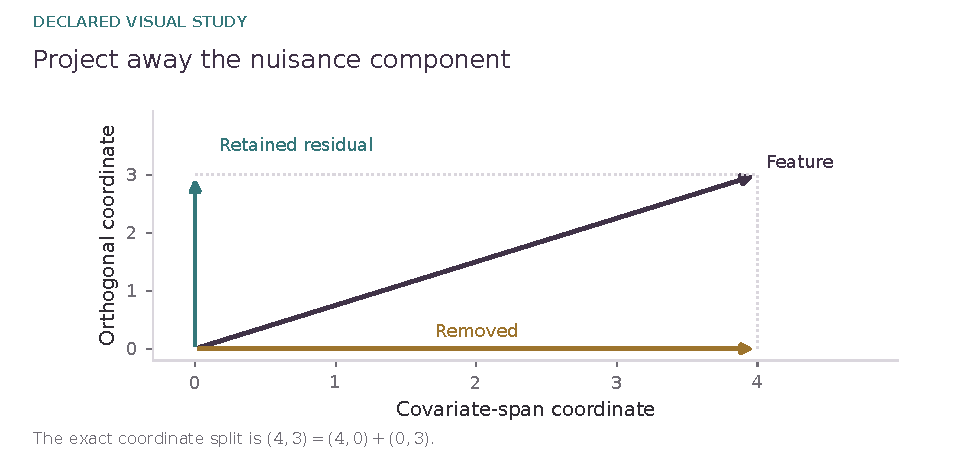
\includegraphics[width=\linewidth]{figures_production/04_residualization.pdf}\end{center}
{\small\color{navy}An exact two-coordinate projection splits a feature into removed and retained components.}

\[Q_X^{\mathsf T}Q_X=I,\quad M_X=I-Q_XQ_X^{\mathsf T},\quad M_X^2=M_X=M_X^{\mathsf T}.\]
\[A=M_XGW^{1/2},\qquad K=AA^{\mathsf T}.\]
For a covariate range basis $Q_X$ with orthonormal columns, the residualizer $M_X=I-Q_XQ_X^{\mathsf T}$ removes the component in the covariate span. It is symmetric and idempotent. Applying it to the weighted feature factor restricts the kernel to variation left after the null-model covariates have been removed.

The two-coordinate control draws the exact split $(4,3)=(4,0)+(0,3)$. The horizontal axis represents the covariate span and the vertical axis its orthogonal complement. This picture explains the geometry. The general projector acts in the full sample space.

The factor $A=M_XGW^{1/2}$ is one specialization of the domain-independent engine. A correct range basis must represent the actual covariate span. Rank deficiency cannot be handled by silently treating extra QR columns as covariate directions.

\studyresult{The general engine operates on factors. Residualized weighted features provide one important factor construction.}
\vfill{\footnotesize\color{navy}\textbf{Reading connection.} Chapter~\ref{ch:streaming}.}
\clearpage
\atlasheading{05}{Structural locality}{Exact zeros create a finite phase cone}
\vspace{3pt}
\begin{center}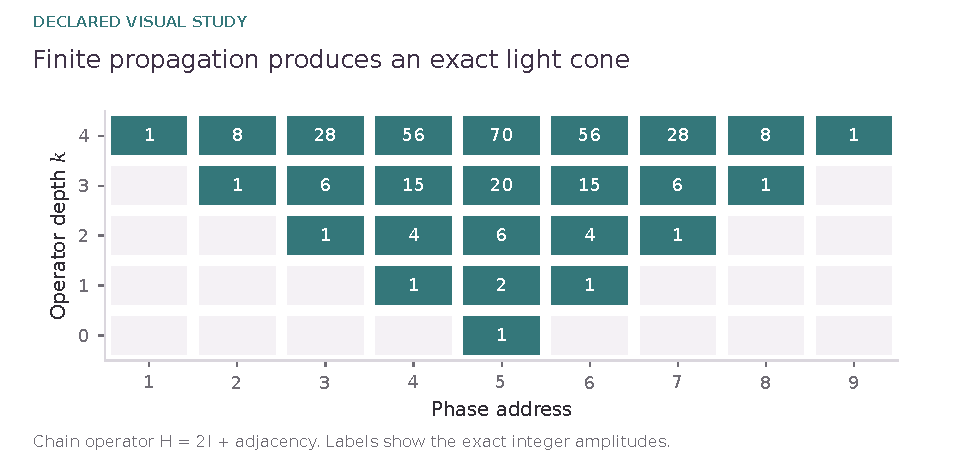
\includegraphics[width=\linewidth]{figures_production/05_phase_cone.pdf}\end{center}
{\small\color{navy}Exact integer phase support for depths zero through four. A colored entry is genuinely nonzero.}

\[\sum_hP_h=I,\qquad g\to h\iff P_hHP_g\ne0.\]
\[\operatorname{dist}(g,h)>k\quad\Longrightarrow\quad P_hH^kP_g=0.\]
Choose a complete orthogonal family of phase projectors on feature space and form $H=A^{\mathsf T}A$. An edge from phase $g$ to phase $h$ exists when the transfer block $P_hHP_g$ is nonzero. Each operator application follows one graph edge. An iterate of depth $k$ cannot reach a phase farther than $k$ edges away.

The finite control is a nine-phase chain with $H=2I+S+S^{\mathsf T}$ and a unit start in phase five. The printed entries are exact integers in $H^kx$, and the shaded support expands by one phase at each step. The script checks every zero outside the cone.

These exact zeros justify omitting inactive phases for that finite-depth query. Storage blocks may still subdivide each active phase arbitrarily. The phase graph answers propagation questions, while the storage partition answers residence questions.

\studyresult{A certified zero allows exact omission. A merely small coupling needs an error bound.}
\vfill{\footnotesize\color{navy}\textbf{Reading connection.} Chapter~\ref{ch:phases}.}
\clearpage
\atlasheading{06}{Approximate locality}{Weak edges need a transfer envelope}
\vspace{3pt}
\begin{center}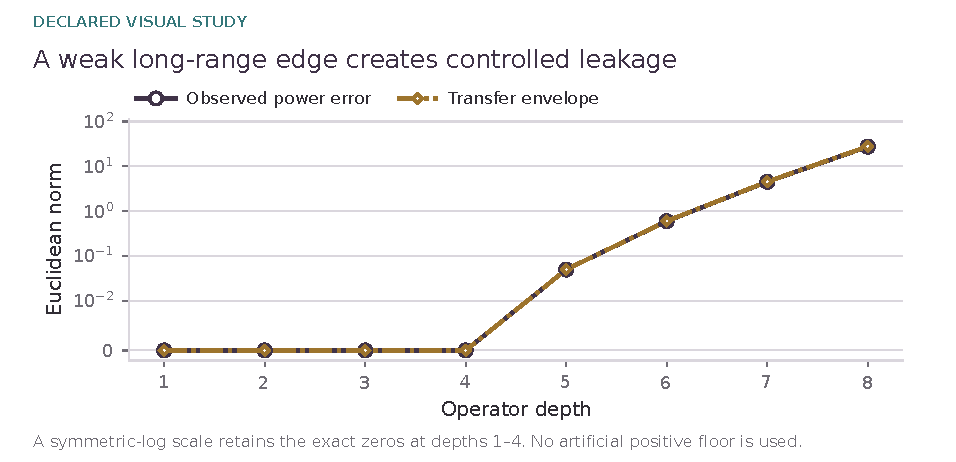
\includegraphics[width=\linewidth]{figures_production/06_approximate_cone.pdf}\end{center}
{\small\color{navy}One declared weak-edge control. A symmetric-log axis keeps exact zeros at zero rather than assigning a positive display floor.}

\[\rho(X)_h=\|P_hX\|_F,\qquad \mathcal B_{hg}=\|P_hHP_g\|_2.\]
\[\rho(H^kX)\le\mathcal B^k\rho(X),\qquad\rho((H^k-H_0^k)X)\le(\mathcal B^k-\mathcal B_0^k)\rho(X).\]
A weak nonzero coupling destroys the exact-zero conclusion. Record the spectral norm of every phase block in a nonnegative transfer matrix $\mathcal B$. The phase-norm profile of any block vector is dominated componentwise by multiplication with $\mathcal B$.

For a retained operator $H_0$, let $\mathcal B_0$ keep the corresponding entries. Telescoping the two operator powers gives a phasewise bound on the omitted action. Symmetric block retention preserves self-adjointness. The power estimate itself does not require the retained operator to be positive.

The toy chain receives a signed weak edge of weight $-0.035$ between phases one and nine. Starting in phase five, that edge has no effect through depth four. At later depths the figure compares floating observed error with the transfer-envelope evaluation. The theorem supplies the general bound. The plot checks this finite instance.

\studyresult{Approximate locality produces a budgeted leakage quantity, not an exact support assertion.}
\vfill{\footnotesize\color{navy}\textbf{Reading connection.} Chapter~\ref{ch:phases}.}
\clearpage
\atlasheading{07}{Core and residual}{The unresolved range has positive structure}
\vspace{3pt}
\begin{center}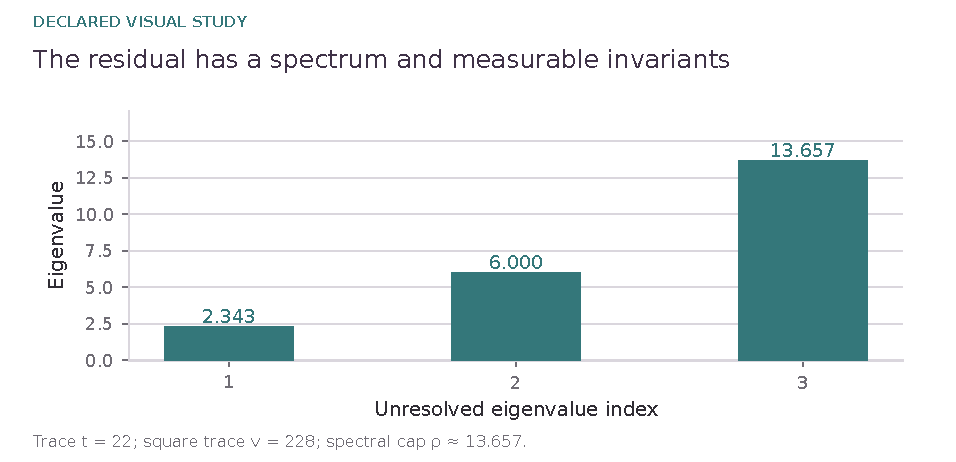
\includegraphics[width=\linewidth]{figures_production/07_residual.pdf}\end{center}
{\small\color{navy}Positive residual coefficients and their invariants for a declared coordinate-range control.}

\[A=UB+F,\quad U^{\mathsf T}F=0,\quad A^{\mathsf T}A=B^{\mathsf T}B+F^{\mathsf T}F.\]
\[t=\operatorname{tr}R=\|F\|_F^2,\quad v=\operatorname{tr}(R^2),\quad \rho_R=\|R\|_2.\]
Let $U$ contain $d$ orthonormal sample-space directions. Project the factor into its captured range coordinates $B=U^{\mathsf T}A$ and residual $F=(I-UU^{\mathsf T})A$. Orthogonality eliminates the cross terms in the feature-space Gram matrix.

The missing term is the positive operator $R=F^{\mathsf T}F$. Its trace is the missing mean of the Gaussian quadratic form. Its square trace measures concentration, and its spectral norm caps any unresolved coefficient. These invariants convey more information than one generic operator-norm error.

The control captures the first three coordinate directions of the integer factor. Its Gram decomposition is checked exactly. Residual eigenvalues and the cap are floating diagnostics. A small residual norm alone does not prove that an extreme-tail probability has the requested relative accuracy.

\studyresult{Unresolved spectral mass is an explicit object with its own trace, concentration, and cap.}
\vfill{\footnotesize\color{navy}\textbf{Reading connection.} Chapter~\ref{ch:spectrum}.}
\clearpage
\atlasheading{08}{Exact completion}{A small remaining range can be completed}
\vspace{3pt}
\begin{center}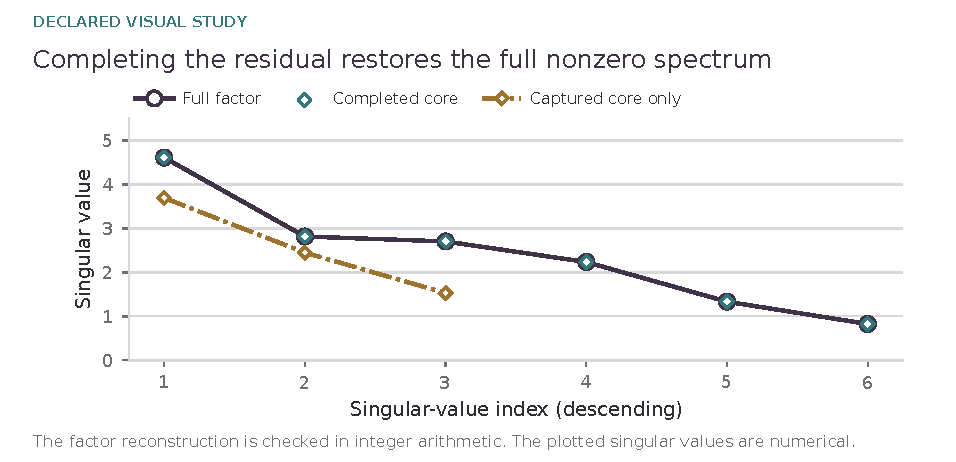
\includegraphics[width=\linewidth]{figures_production/08_completion.pdf}\end{center}
{\small\color{navy}Completed and full singular spectra coincide in the integer factor control. The captured core is incomplete.}

\[U^{\mathsf T}W=0,\qquad A=[U\ W]\begin{bmatrix}B\\D\end{bmatrix}.\]
\[\left\lceil\max\{t/\rho_R,t^2/v\}\right\rceil\le\operatorname{rank}F\le n-d\quad(F\ne0).\]
If the residual admits $F=WD$ with orthonormal columns of $W$, its range lies orthogonal to $U$. Appending $W$ therefore creates an orthonormal synthesis factor, and stacking the two coordinate cores recovers the full factor.

The nonzero singular values of the completed core equal those of the original factor. The figure compares the incomplete captured core with the completed core in the declared integer example. Exact reconstruction of that factor is checked before numerical singular values are plotted.

Residual moments also provide a rank lower bound. Together with the orthogonal-complement dimension they can identify the missing rank when the two integers agree. A completion procedure must retain all genuine residual directions. A floating rank threshold has a separate error obligation.

\studyresult{When the remaining rank is affordable, exact completion can replace further approximate iteration.}
\vfill{\footnotesize\color{navy}\textbf{Reading connection.} Chapter~\ref{ch:spectrum}.}
\clearpage
\atlasheading{09}{Probability reweighting}{Tilting moves the query into the bulk}
\vspace{3pt}
\begin{center}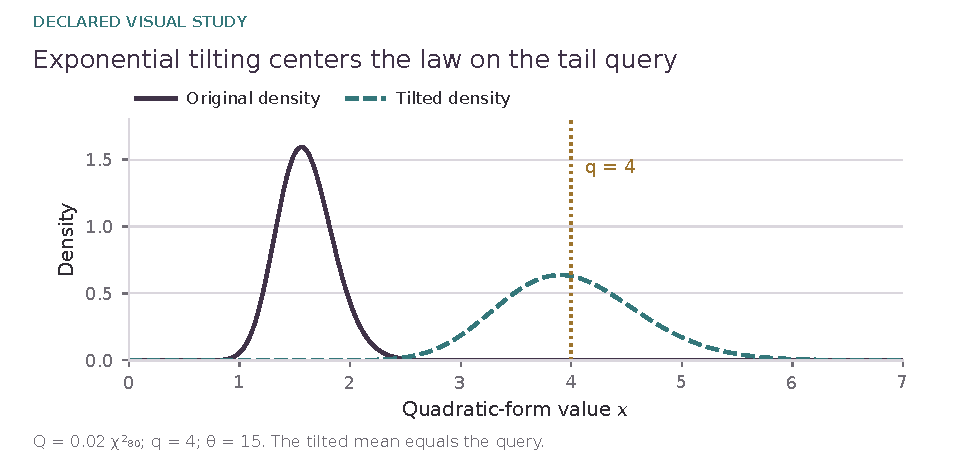
\includegraphics[width=\linewidth]{figures_production/09_tilt.pdf}\end{center}
{\small\color{navy}The threshold becomes central under the tilted law. The likelihood-ratio weight restores the original tail.}

\[\kappa(s)=-\frac12\sum_j\log(1-2s\lambda_j),\qquad 0<\theta<\frac1{2\lambda_{\max}}.\]
\[P(Q\ge q)=e^{\kappa(\theta)-\theta q}\,\mathbb E_\theta[e^{-\theta(Q-q)}\mathbf1_{\{Q\ge q\}}].\]
For a positive spectrum, the cumulant generating function is a sum of logarithms. A real tilt inside its domain defines a normalized reweighted law. The original upper tail becomes an exponential prefactor times a bounded weighted expectation under that law.

For an upper-tail planner query $q>\mathbb E Q$, the saddlepoint solves $\kappa'(\theta)=q$. It centers the tilted law at the threshold and often improves numerical efficiency. The enclosure identity holds for any admissible positive tilt. Certification does not require solving the saddlepoint exactly.

The figure uses $Q=0.02\chi^2_{80}$ and $q=4$. Its original mean is $1.6$, while the tilted mean is $4$ at $\theta=15$. The plotted densities follow the same exact gamma family with different scales. No approximation to the probability law is introduced by tilting.

\studyresult{Use the tilt to condition the calculation. Retain the exact reweighting identity to preserve the target probability.}
\vfill{\footnotesize\color{navy}\textbf{Reading connection.} Chapter~\ref{ch:packets}.}
\clearpage
\atlasheading{10}{Local transform representation}{A spectral packet stores centered moments}
\vspace{3pt}
\begin{center}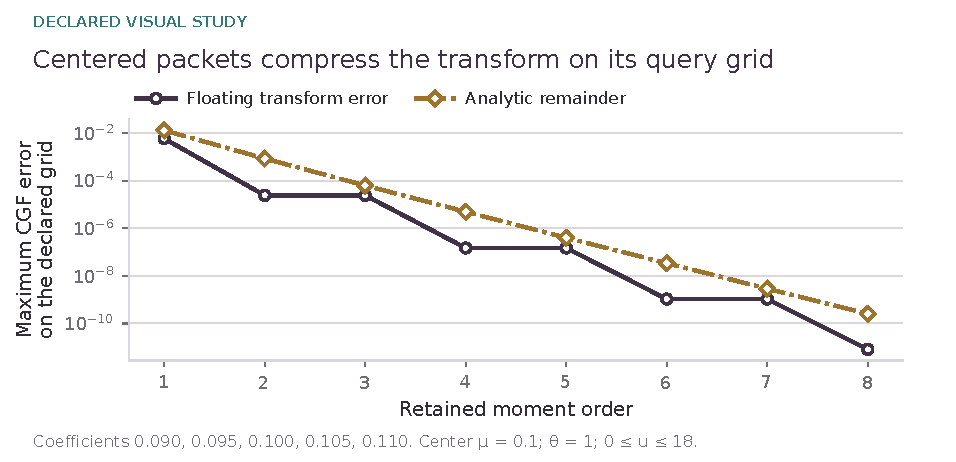
\includegraphics[width=\linewidth]{figures_production/10_packet.pdf}\end{center}
{\small\color{navy}Centered storage and the declared-grid remainder ladder for one finite packet.}

\[M_{P,m}=\sum_{j\in P}(\lambda_j-\mu_P)^m,\quad\alpha_P(s)=\frac{2s}{1-2s\mu_P},\quad\rho_P(s)=|\alpha_P(s)|\max_{j\in P}|\lambda_j-\mu_P|.\]
\[\kappa_P(s)=-\frac{n_P}{2}\log(1-2s\mu_P)+\frac12\sum_{m=1}^{p}\frac{\alpha_P(s)^m M_{P,m}}m+R_{P,p}(s),\]
\[|R_{P,p}(s)|\le\frac{n_P}{2}\frac{\rho_P(s)^{p+1}}{(p+1)(1-\rho_P(s))}.\]
The packet stores nearby eigenvalues through their mean $\mu_P$ and centered power sums $M_{P,m}$, with $M_{P,1}=0$. It expands the log transform rather than substituting a surrogate distribution.

Use a nonempty positive packet, integer order $p\ge0$, and $\Re s<1/(2\lambda_{\max})$. The factor logarithms use their principal branches and sum to the analytic $\kappa$ normalized at zero. For $\rho_P(s)<1$, the series has the stated remainder, which decreases geometrically when the radius ratio stays away from one.

The five-eigenvalue control uses $0.09,0.095,0.10,0.105,0.11$, a tilt of one, and 220 frequencies from zero to eighteen. The figure compares floating transform errors with the analytic remainder at orders one through eight. These computations illustrate the bound. They do not enclose library rounding.

\studyresult{The local packet representation requires the transform domain, logarithm branch, and printed radius condition.}
\vfill{\footnotesize\color{navy}\textbf{Reading connection.} Chapter~\ref{ch:packets}.}
\clearpage
\atlasheading{11}{Grid-dependent compilation}{The query determines the useful packet}
\vspace{3pt}
\begin{center}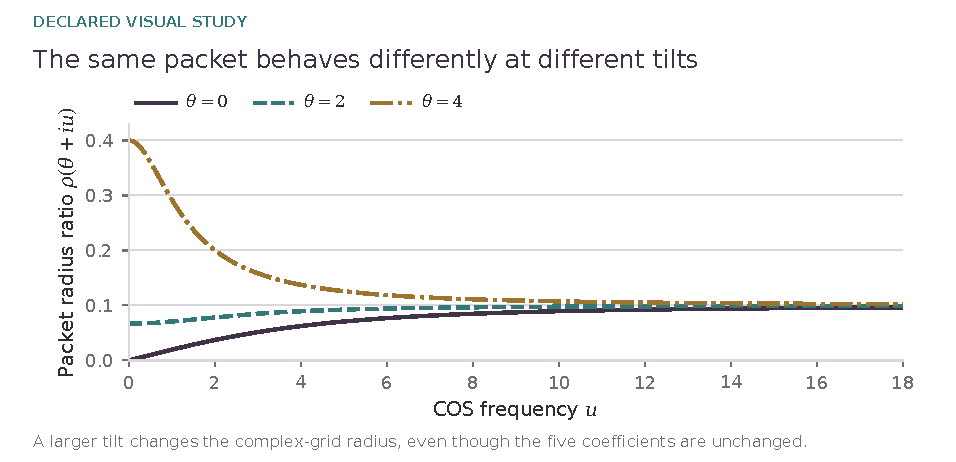
\includegraphics[width=\linewidth]{figures_production/11_query_grid.pdf}\end{center}
{\small\color{navy}The same spectral packet has different expansion ratios at tilts zero, two, and four.}

\[s_k=\theta+i\frac{k\pi}{b},\qquad\rho_P(s_k)<1\quad\text{on every retained frequency}.\]
\[(\Lambda,q,\varepsilon)\longmapsto\mathcal P_{\Lambda,q,\varepsilon}.\]
A distance between eigenvalues is insufficient to decide whether a packet is useful. The expansion must be controlled at the actual complex arguments $s_k=\theta+i k\pi/b$ selected by the tail query. The tilt, support endpoint, and retained mode count all change that grid.

The figure holds the same five eigenvalues and packet center fixed while changing the tilt. Near the transform singularity the low-frequency radius can grow sharply. At high frequency the radius approaches the relative packet half-width. Neither effect is captured by inspecting raw eigenvalue spacing alone.

The compiled representation may retain large spikes exactly and packetize a smooth spectral bulk. Split a packet or raise its order when its propagated error exceeds budget. A plan can be reused only after checking that its stored conditions and grid remain applicable to the new request.

\studyresult{The passport belongs to a spectrum, a query, and an accuracy contract, rather than to the spectrum alone.}
\vfill{\footnotesize\color{navy}\textbf{Reading connection.} Chapter~\ref{ch:packets}.}
\clearpage
\atlasheading{12}{Finite-window transform}{Cosine inversion integrates a weighted tail}
\vspace{3pt}
\begin{center}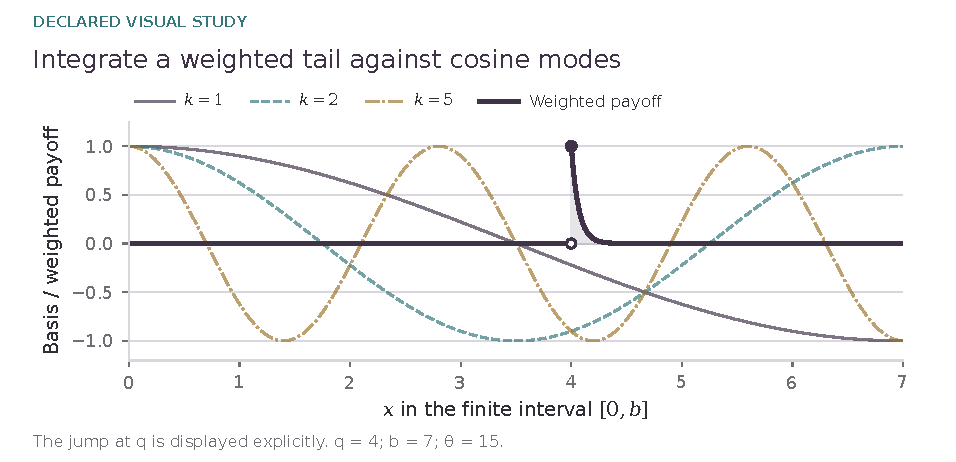
\includegraphics[width=\linewidth]{figures_production/12_cos.pdf}\end{center}
{\small\color{navy}The weighted payoff and finite-interval basis have different roles. The prime gives half weight to mode zero.}

\[J_k=\int_q^be^{-\theta(x-q)}\cos(u_kx)\,dx=\Re\!\left[e^{iu_kq}\frac{1-e^{(-\theta+iu_k)(b-q)}}{\theta-iu_k}\right].\]
\[S_N=\frac2b\sum_{k=0}^{N-1}{}^{\prime}\, J_k\,\Re\,\phi_\theta(u_k),\qquad\phi_\theta(t)=e^{\kappa(\theta+it)-\kappa(\theta)}.\]
On a positive-support interval $[0,b]$, the cosine frequencies are $u_k=k\pi/b$. The payoff is zero below the threshold and decays exponentially above it. Integrating each cosine mode against that payoff gives an explicit coefficient.

The finite sum uses the tilted characteristic function rather than a CDF value close to one. Multiplying by the likelihood-ratio prefactor returns the original tail scale. This avoids subtracting two almost equal numbers, but it does not remove the need to bound discarded support and omitted modes.

The picture uses $q=4$, $b=7$, and $\theta=15$. The payoff and three cosine modes share one coordinate system, with distinct line styles and an explicit payoff discontinuity. Correctness of the positive-support backend requires $q\ge0$ and $b>q$. The saddlepoint planner additionally selects upper-tail queries above the original mean.

\studyresult{A finite-window, finite-mode transform is an intermediate quantity whose omitted contributions require bounds.}
\vfill{\footnotesize\color{navy}\textbf{Reading connection.} Chapter~\ref{ch:inversion}.}
\clearpage
\atlasheading{13}{Omitted Fourier modes}{Mode decay bounds the infinite remainder}
\vspace{3pt}
\begin{center}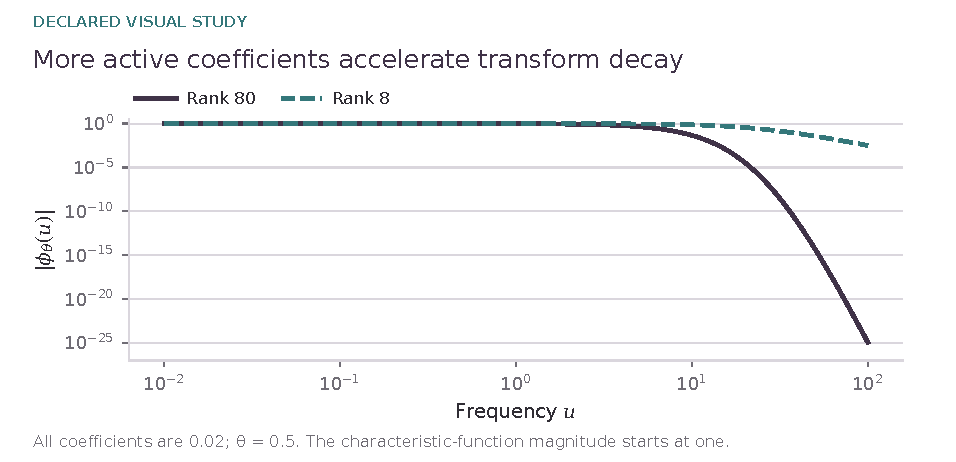
\includegraphics[width=\linewidth]{figures_production/13_mode_decay.pdf}\end{center}
{\small\color{navy}Declared equal-coefficient controls illustrate why the number of active coefficients affects high-frequency decay.}

\[a_j=\frac{2\lambda_j}{1-2\theta\lambda_j},\quad|\phi_\theta(t)|=\prod_j(1+(a_jt)^2)^{-1/4}\le C_\theta t^{-r/2}.\]
\[E_{\rm series}\le\frac{2C_\theta}{b\theta}\left(\frac b\pi\right)^\nu\left[N^{-\nu}+\frac{N^{1-\nu}}{\nu-1}\right],\quad\nu=r/2>1.\]
The modulus of the normalized tilted characteristic function has a positive product formula. Its decay is controlled by the actual transformed coefficients. More active positive coefficients increase the asymptotic decay exponent.

The figure compares eight and eighty equal coefficients at the same admissible tilt. It evaluates the exact modulus formula in ordinary floating arithmetic. A rapidly falling curve is useful for choosing modes, but acceptance depends on a proved bound for the entire omitted series.

The rigorous interval backend uses a simple envelope $C_\theta t^{-r/2}$ and the payoff bound $|J_k|\le1/\theta$. Its resulting series bound requires $r>2$. The packetized analytic path has a sharper frequency-dependent decay-rate bound. Those are distinct formulas with distinct implementation scopes.

\studyresult{The infinite-mode remainder is a mathematical tail of a series, separate from floating summation error.}
\vfill{\footnotesize\color{navy}\textbf{Reading connection.} Chapter~\ref{ch:inversion}.}
\clearpage
\atlasheading{14}{Analytic and arithmetic budgets}{The error ledger keeps separate causes}
\vspace{3pt}
\begin{center}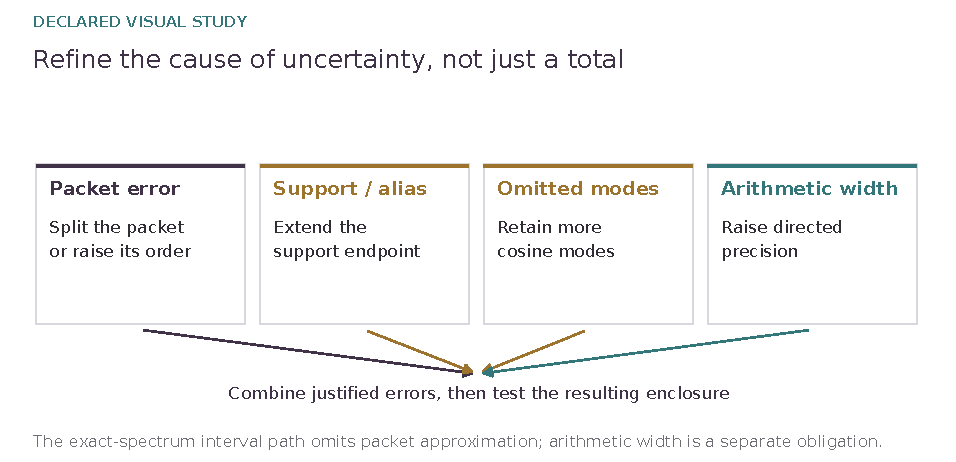
\includegraphics[width=\linewidth]{figures_production/14_ledger.pdf}\end{center}
{\small\color{navy}Four causes of uncertainty and their natural controls. Every budget must be justified before acceptance.}

\[|p-\widehat p|\le E_{\rm packet}+E_{\rm support}+E_{\rm modes}\quad\text{(analytic packet path)}.\]
\[S_\theta(q)\in\boldsymbol S_N+[-E,E],\qquad E=E_{\rm support}+E_{\rm series}\quad\text{(exact-spectrum interval path)}.\]
Packet approximation changes the retained-grid transform. Support truncation and cosine periodization change the finite-window functional. Mode truncation removes infinitely many terms. These three mathematical approximation errors have different refinement controls and must be accounted for separately.

Directed-rounding arithmetic introduces a fourth quantity: the width of the computed interval for finite operations. That width is not a substitute for an analytic remainder. Conversely, an analytic bound does not automatically enclose the rounding of logarithms, exponentials, or summation.

For the exact-spectrum interval backend, no packet approximation is used. The finite transform interval is enlarged by support and series bounds, then passed through a positive logarithm and prefactor enclosure. Extending directed-rounding certification to the packet transform requires enclosing its moment construction and remainder propagation as well.

\studyresult{Name the uncertainty before refining it. The same scalar tolerance can hide different unresolved causes.}
\vfill{\footnotesize\color{navy}\textbf{Reading connection.} Chapter~\ref{ch:inversion}.}
\clearpage
\atlasheading{15}{Requested accuracy}{Acceptance is a logarithmic interval test}
\vspace{3pt}
\begin{center}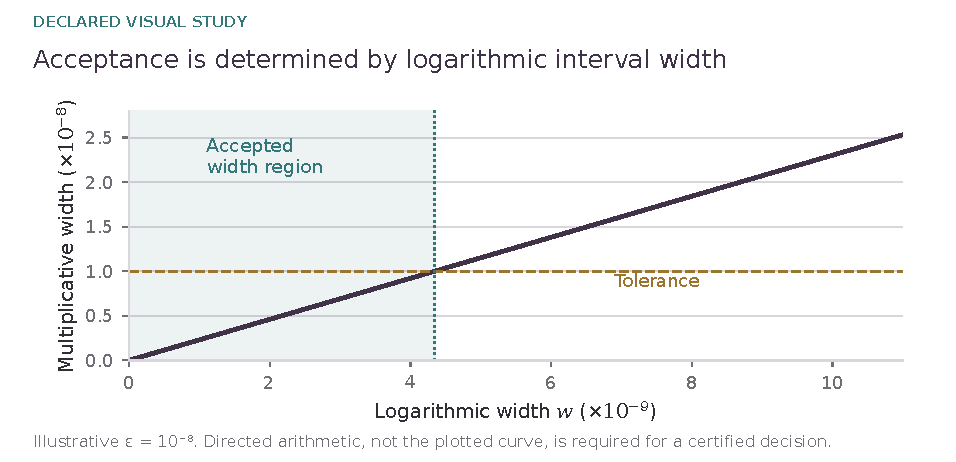
\includegraphics[width=\linewidth]{figures_production/15_acceptance.pdf}\end{center}
{\small\color{navy}An illustrative tolerance of $10^{-8}$ determines the permitted log width. The plotted curve is numerical.}

\[\log_{10}p\in[d_-,d_+],\quad w=d_+-d_-,\quad\frac{p_+}{p_-}-1=\operatorname{expm1}(\log(10)w).\]
\[\operatorname{expm1}(\log(10)w)\le\varepsilon\quad\Longrightarrow\quad\text{requested enclosure width is met}.\]
A positive probability enclosure can be stored on a logarithmic scale even when its endpoints are below ordinary floating-point range. If $d_-$ and $d_+$ enclose $\log_{10}p$, the width determines the maximum multiplicative uncertainty.

For validated acceptance, compute the width and $\operatorname{expm1}(\log(10)w)$ with directed interval arithmetic. Compare the ratio interval\textquotesingle s upper endpoint to the exact tolerance enclosure\textquotesingle s lower endpoint. Preserve the literal outer endpoints throughout parsing and conversion. High precision alone does not prove this decision.

The controller returns an accepted result only after the full enclosure passes the requested tolerance. An unresolved positive lower bound, invalid transform domain, inadequate mode budget, or exhausted precision budget must produce a failure status. A point estimate can still be informative, but it cannot be relabeled as an accepted enclosure.

\studyresult{The decision logic and input semantics are part of certification, just as the transform arithmetic is.}
\vfill{\footnotesize\color{navy}\textbf{Reading connection.} Chapter~\ref{ch:accuracy}.}
\clearpage
\atlasheading{16}{Independent control family}{An exact-law control reaches deep logarithms}
\vspace{3pt}
\begin{center}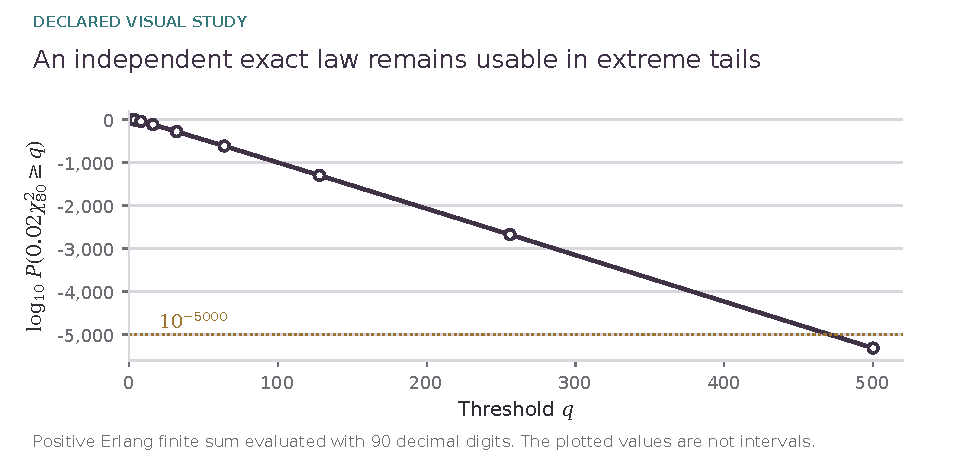
\includegraphics[width=\linewidth]{figures_production/16_exact_control.pdf}\end{center}
{\small\color{navy}An independently evaluable exact-law family. The plot is regenerated from a positive finite sum in decimal arithmetic.}

\[z=q/0.04,\qquad P(Q\ge q)=e^{-z}\sum_{k=0}^{39}\frac{z^k}{k!}.\]
\[\log_{10}P(Q\ge q)=\frac{-z+\log\!\left(\sum_{k=0}^{39}z^k/k!\right)}{\log(10)}.\]
For an even-degree chi-square variable, the upper tail has a finite positive-sum formula. The control $Q=0.02\chi^2_{80}$ is a gamma law of integer shape forty and scale $0.04$. Its survival probability can therefore be evaluated independently of cosine inversion.

The curve computes the logarithm first. At thresholds from $1.6$ through $500$, it evaluates the finite sum with ninety decimal digits and plots its logarithm. The exact law supplies the formula. The numeric points are high-precision evaluations rather than directed-rounding enclosures.

This control can distinguish a transform error from a reference error without relying on another COS run. Its equal-coefficient structure also means that one packet can represent the spectrum exactly. Success on this family does not establish equal performance for heterogeneous spectra, signed laws, or every matrix-to-spectrum bridge.

\studyresult{Choose a reference with a different mathematical route. Report its arithmetic scope alongside the result.}
\vfill{\footnotesize\color{navy}\textbf{Reading connection.} Chapter~\ref{ch:intervals}.}
\clearpage
\atlasheading{17}{Publication and evidence map}{Read each evidence layer on its own terms}
\vspace{3pt}
\vspace{5pt}\begin{center}\small\renewcommand{\arraystretch}{1.3}\begin{tabular}{@{}>{\raggedright\arraybackslash}P{.25\linewidth}>{\raggedright\arraybackslash}P{.33\linewidth}>{\raggedright\arraybackslash}P{.36\linewidth}@{}}\toprule
Representation layer & Evidence to inspect & Scope to preserve\\
\midrule
Block / projector algebra & Exact identities. Selected Lean sources & All required hypotheses and finite dimensions\\
Computed spectrum & Validated matrix-to-spectrum bridge & Input semantics. Residual and rounding enclosures\\
Spectral packet transform & Analytic remainders. Executable checks & Complex-grid radius. Arithmetic error\\
Positive exact-spectrum tail & Directed-rounding interval. Analytic bounds & Admissible tilt. Positive support. Active rank\\
Controller decision & Enclosure-width test. Precision and parsing tests & Requested tolerance. Explicit failure status\\
\bottomrule\end{tabular}\end{center}
\[\text{matrix input}\ \longrightarrow\ \text{spectral enclosure}\ \longrightarrow\ \text{tail enclosure}\ \longrightarrow\ \text{accepted width}.\]
The main chapters explain the operator identities, propagation bounds, residual structure, packet construction, and probability enclosures. The atlas makes those mechanisms inspectable through small declared cases. The formalization appendix identifies exactly which finite-algebra or order statements are represented by its source files and what the checked build establishes.

A Lean proof of block matrix algebra does not automatically certify a Python eigensolver, a decimal parser, or a transcendental interval library. A directed-rounding tail computation for exact supplied coefficients does not automatically certify coefficients computed by an unverified SVD. Each interface needs its own evidence.

The accompanying package preserves executable sources and verification records. Rebuild the figures with \decl{illustrations/production_figures.py}, inspect its input manifest, and compare the formalization guide with its checked sources. All illustrations use declared controls, and no empirical timing or production tail claim is introduced by this atlas.

\studyresult{A complete result carries its assumptions, representation semantics, numerical enclosure, and formal scope.}
\vfill{\footnotesize\color{navy}\textbf{Reading connection.} Appendix~\ref{app:lean}.}

\endgroup

\bookmarksetup{startatroot}
\chapter{Formalization and theorem correspondence}\label{app:lean}
The formal companion covers exact finite Gram algebra, disjoint block
refinement, reindexing, streamed actions, nonnegativity, coefficient order,
and arithmetic consequences of supplied enclosures. It does not establish
the Gaussian reduction, Fourier inversion, analytic remainders, spectral
post-verification algorithm, or transcendental interval-library correctness.
A theorem that assumes an enclosure does not construct that enclosure.

\begin{scopebox}
\textbf{Recorded kernel evidence.} The retained compiler record accepts
26 theorem declarations and 8 definitions, with a 34-declaration axiom audit.
The audited dependencies are confined to \texttt{propext},
\texttt{Classical.choice}, and \texttt{Quot.sound}. No \texttt{sorryAx} or
custom axiom appears. A valid arithmetic control was accepted, while false
arithmetic and an acceptance proof missing its error-budget premise were
rejected. This volume preserves that evidence and the pinned sources. It
does not claim a new Lean compilation.
\end{scopebox}

\label{app:lean-contract}
\section{How the formal model represents the engine}

The factor has a finite sample index type $I$ and an arbitrary variant index
 type $V$. A variant block is a finite set $s\subseteq V$. The factor entries
are exact real numbers, $A:I\times V\to\R$. The Lean type is
\decl{Row -> Variant -> Real}. The sample coordinates carry a
\decl{Fintype} instance. The variants carry a \decl{DecidableEq} instance to
support finite-set unions, singleton blocks, and reindexing.

The residualized weighted factor in the main text is
\[
 A=M_X G W^{1/2}.
\]
For this companion, $A$ is supplied. Proving that a particular floating-point
residualization procedure computes that mathematical factor would require
additional implementation and numerical-error reasoning. These modules do
not assume a covariance model or a distribution for the vector $v$.

There are five central finite-algebra definitions:
\begin{align*}
 \operatorname{gramEntry}(s,A,i,j)&=\sum_{k\in s}A_{ik}A_{jk},\\[6pt]
 \operatorname{matrixAction}(K,v,i)&=\sum_{j\in I}K_{ij}v_j,\\[6pt]
 \operatorname{streamedAction}(s,A,v,i)&=\sum_{k\in s}A_{ik}\sum_{j\in I}A_{jk}v_j,\\[6pt]
 \operatorname{quadraticForm}(K,v)&=\sum_{i\in I}v_i\operatorname{matrixAction}(K,v,i),\\[6pt]
 \operatorname{factorEnergy}(s,A,v)&=\sum_{k\in s}\left(\sum_{i\in I}A_{ik}v_i\right)^2.
\end{align*}
The source uses ordinary finite sums in $\R$. The factor convention is the
sample Gram $AA^\top$, matching \decl{stream_sample_gram}. It is not the dual
Gram $A^\top A$. The case-study statistic $Q=\tfrac12 v^\top Kv$ requires the
additional scalar factor $\tfrac12$ when applying these identities.

\section{Exact block refinement}

The principal refinement theorem is \decl{gramEntry_union}. Its hypotheses
are finite sets $s,t\subseteq V$ and $\operatorname{Disjoint}(s,t)$. It proves,
for all sample coordinates $i,j$,
\[
 \operatorname{gramEntry}(s\cup t,A,i,j)
 =\operatorname{gramEntry}(s,A,i,j)+\operatorname{gramEntry}(t,A,i,j).
\]
Disjointness prevents repeated columns from being counted twice. It is a
mathematical condition, not a performance assumption. The theorem applies to
empty blocks and zero factors. It does not require positive weights, since
$A$ is already supplied as a real factor.

The proof unfolds \decl{gramEntry} and invokes the finite-sum union identity.
No numerical approximation is involved. Repeated application establishes
invariance along any explicitly checked sequence of binary disjoint splits.
The source does not encode a whole scheduler or its memory allocation policy.
A scheduler correctness proof would additionally track complete coverage,
disjointness, and termination at every split.

The same refinement has formal consequences for the operator action and the
quadratic statistic:
\begin{align*}
 (K_{s\cup t}v)_i&=(K_s v)_i+(K_t v)_i,\\
 v^\top K_{s\cup t}v&=v^\top K_s v+v^\top K_t v.
\end{align*}
These are \decl{matrixAction_gram_union} and
\decl{quadraticForm_gram_union}. The independent
\decl{streamedAction_union} proves the corresponding streamed accumulation
identity directly.

The reindexing theorem \decl{gramEntry_reindex} handles a bijection
$e:V\simeq V$. It moves the block to $e(s)$ and transforms the factor to
$A'_{ik}=A_{i,e^{-1}(k)}$. The resulting Gram entry is unchanged. Permuting
only the coordinates without moving their factor columns falls outside this
statement.

\section{Streamed actions and the sum-of-squares identity}

\decl{matrixAction_gram_eq_streamed} proves
\[
 \sum_{j\in I}\left(\sum_{k\in s}A_{ik}A_{jk}\right)v_j
 =\sum_{k\in s}A_{ik}\left(\sum_{j\in I}A_{jk}v_j\right).
\]
This is the exact algebra behind multiplication by a sample Gram matrix
without constructing that matrix. Lean checks the finite-sum interchange and
associativity of real multiplication. It does not assert that a given
sequence of device operations has exact real semantics.

The next theorem, \decl{quadraticForm_gram_eq_energy}, proves
\[
 v^\top K_s v=\sum_{k\in s}\left(\sum_{i\in I}A_{ik}v_i\right)^2.
\]
It expands the action, interchanges the finite sums, factors each coordinate
sum, and identifies the product of a projection with itself. The resulting
\decl{quadraticForm_gram_nonneg} states $0\le v^\top K_s v$ for every real
vector $v$. This is positive semidefiniteness of the supplied Gram form.

These identities are useful together. Refinement preserves the represented
operator, streaming preserves its action, and the energy identity verifies
its positivity. They do not require the eigenvalues or the spectral theorem.
The full engine subsequently uses numerical rank compression and spectral
information, whose correctness contracts are separate.

\section{A complete exact algebra example}

Consider one sample coordinate and two variant columns with
\[
 A=(3\quad4),\qquad v=2.
\]
The two singleton Gram contributions are $9$ and $16$. Their disjoint union
has Gram entry $25$. Matrix multiplication gives $Kv=50$ and
$v^\top Kv=100$. The streamed action instead computes
\[
 3(3\cdot2)+4(4\cdot2)=18+32=50.
\]
The energy expression gives
\[
 (3\cdot2)^2+(4\cdot2)^2=36+64=100.
\]
Thus the engine statistic with the stated half normalization is $Q=50$.
All paths are exact real identities. This example explains the type and
normalization choices. The universal theorems establish them for arbitrary
finite sample coordinates and variant blocks.

If the two blocks overlap in one column, their sum repeats that column's
outer product. For $s=t=\{1\}$ and $A_{i1}=3$, the union has contribution $9$
while the sum of the two blocks is $18$. This is why
\decl{gramEntry_union} requires disjointness.

\section{Supplied coefficient intervals}

The separate definition
\[
 \operatorname{weightedSquares}(s,c,z)=\sum_{k\in s}c_k z_k^2
\]
models a supplied diagonal quadratic form. Its coefficients need not be
eigenvalues obtained by a proved diagonalization. It has three theorems:
\begin{itemize}
 \item \decl{weightedSquares_mono}: if $l_k\le u_k$ for every $k\in s$, then
 $\sum l_kz_k^2\le\sum u_kz_k^2$.
 \item \decl{weightedSquares_nonneg}: if $c_k\ge0$ for every $k\in s$, then
 $\sum c_kz_k^2\ge0$.
 \item \decl{weightedSquares_tail_imp}: coefficientwise order gives the
 pointwise implication $q\le\sum l_kz_k^2\Rightarrow q\le\sum u_kz_k^2$.
\end{itemize}
The first and third allow signed coefficients because squares remain
nonnegative. The second has an explicit nonnegativity hypothesis.

The pointwise implication is a prerequisite for probabilistic tail
sandwiching. It does not itself state a probability inequality or build a
coupling. To turn it into such a statement, one must supply measurable random
coordinates on a common probability space and use monotonicity of measure.
To apply it to matrix spectra, one must also establish that each true
coefficient lies inside the supplied interval.

\section{Enclosures and error ledgers}

The interval module uses two elementary predicates:
\begin{align*}
 \operatorname{Enclosed}(x,L,U)&\;:\Longleftrightarrow\;L\le x\le U,\\
 \operatorname{ErrorBound}(x,\widehat x,r)&\;:\Longleftrightarrow\;
 |x-\widehat x|\le r.
\end{align*}
The equivalence \decl{errorBound_iff_enclosed} proves
\[
 |x-\widehat x|\le r
 \quad\Longleftrightarrow\quad
 \widehat x-r\le x\le\widehat x+r.
\]
There is no extra nonnegativity hypothesis: if this predicate holds, then the
radius is necessarily nonnegative. The definition accepts arbitrary real
inputs, and the theorem states the exact logical equivalence.

For the K-COS error ledger, distinguish the ideal analytic quantity $x$, an
exact finite transform $m$, and the computed estimate $\widehat x$. If
\[
 |x-m|\le a,\qquad |m-\widehat x|\le b,
\]
then \decl{errorBound_compose} proves
\[
 |x-\widehat x|\le a+b.
\]
The proof is the triangle inequality. The hypotheses must be proved
independently. In particular, $a$ can contain a support/alias bound and an
omitted-mode bound. This theorem only composes those supplied facts.

\decl{errorBound_accept} adds the hypothesis $a+b\le\varepsilon$ and concludes
$|x-\widehat x|\le\varepsilon$. This is the arithmetic core of acceptance by a
proved budget. A sequence of numerically stable estimates, without valid
bounds, does not satisfy its hypotheses.

\section{Safe transformations of an enclosure}

The remaining interval statements are reusable exact-real rules.
\decl{enclosed_add} adds two enclosed quantities.
\decl{enclosed_scale} scales the interval by a nonnegative real factor.
\decl{enclosed_widen} permits an explicitly wider interval.
\decl{enclosed_intersect} combines two independently valid enclosures of the
same quantity using $\max$ on the lower endpoints and $\min$ on the upper
endpoints.

\decl{enclosed_positive} requires a strictly positive lower endpoint. It then
proves that the enclosed quantity is positive. This is relevant before
applying a logarithm to a corrected tilted finite sum. A lower endpoint equal
to zero does not establish positivity.

Finally, \decl{enclosed_monotone} transports an interval through a supplied
monotone function. Its hypothesis is global monotonicity on $\R$. The source
does not directly instantiate this rule with the real logarithm, which needs
a positive-domain formulation. A log-tail certificate therefore still needs
both positivity and a separate domain-correct monotonicity argument. The
interval-library implementation also requires its own correctness contract.

\section{Declaration inventory and theorem correspondence}

All names below are prefixed by \decl{KomorebiQCOS}. The inventory counts
project theorems only. Imported mathlib theorems are not counted.

{\small
\begin{longtable}{@{}P{0.49\linewidth}P{0.45\linewidth}@{}}
\toprule Declaration & Exact formal scope\\\midrule\endhead
\decl{gramEntry_empty} & Empty variant block gives zero.\\
\decl{gramEntry_singleton} & One column gives its outer product.\\
\decl{gramEntry_symm} & Real Gram entry symmetry.\\
\decl{gramEntry_union} & Disjoint binary block refinement.\\
\decl{gramEntry_reindex} & Factor-column permutation invariance.\\
\decl{matrixAction_gram_eq_streamed} & Gram action equals streamed factor action.\\
\decl{matrixAction_add} & Operator-action additivity.\\
\decl{matrixAction_gram_union} & Action refinement invariance.\\
\decl{streamedAction_union} & Streamed accumulation over disjoint blocks.\\
\decl{quadraticForm_add} & Quadratic-form additivity in the matrix.\\
\decl{quadraticForm_gram_eq_energy} & Gram form equals factor energy.\\
\decl{quadraticForm_gram_nonneg} & Positivity of the supplied Gram form.\\
\decl{quadraticForm_gram_union} & Statistic refinement invariance.\\
\decl{weightedSquares_mono} & Pointwise coefficientwise order.\\
\decl{weightedSquares_nonneg} & Positivity for nonnegative coefficients.\\
\decl{weightedSquares_tail_imp} & Pointwise tail-event implication.\\
\decl{enclosed_order} & A valid enclosure has ordered endpoints.\\
\decl{enclosed_add} & Additive interval composition.\\
\decl{enclosed_scale} & Nonnegative scaling.\\
\decl{enclosed_widen} & Valid interval widening.\\
\decl{enclosed_intersect} & Intersection of valid enclosures.\\
\decl{errorBound_iff_enclosed} & Absolute-error/enclosure equivalence.\\
\decl{errorBound_compose} & Analytic and arithmetic budget composition.\\
\decl{errorBound_accept} & Acceptance below a supplied tolerance.\\
\decl{enclosed_positive} & Positive lower endpoint proves positivity.\\
\decl{enclosed_monotone} & Supplied monotone transformation.\\
\bottomrule
\end{longtable}
}

The exact-block, hierarchical-blocking, and streamed-action sections of the
main text map to the Gram theorems under the definitions above. The
error-ledger and acceptance sections map only to the arithmetic consequences
of already valid bounds. The matrix-to-tail bridge maps to pointwise
coefficient order only. The detailed machine-readable concordance includes
source filenames and implementation anchors.

\section{Reproduction and trusted dependencies}

The companion includes the pinned toolchain and dependency manifest, two
mathematical modules, a root import, an axiom audit, controls, and retained
build logs. From the companion directory, run:
\begin{verbatim}
lake exe cache get
lake build
lake env lean AxiomAudit.lean
\end{verbatim}
Reproduction requires the pinned compiler and dependencies. Compiler
binaries and the mathlib cache are not distributed in this package.
The retained runtime record includes an executable-location adapter and its
source. It did not modify the compiler or proof kernel.

The positive and negative controls supplement the theorem build. The
axiom audit records each declaration's dependencies. Classical choice,
propositional extensionality, and quotient soundness are the reported
foundational dependencies. Any \decl{sorryAx} occurrence would indicate an
admitted proof. A clean admission scan alone does not establish acceptance.
The retained compiler logs and axiom output provide that evidence.

\section{Remaining formal obligations}

An end-to-end formal certificate would also require:
\begin{enumerate}[nosep,topsep=4pt]
 \item Gaussian whitening and central, signed, and noncentral reductions
 under their exact hypotheses.
 \item Spectral decomposition and a proved connection between the input
 matrix, its factor, and coefficient intervals.
 \item Probability monotonicity under a common measurable coupling.
 \item Exponential tilting and the transform/payoff inversion identity.
 \item Support, alias, and omitted-mode bounds with their rank and
 moment-generating-function domain conditions.
 \item Exact interval semantics for input literals, directed rounding,
 roots, complex transforms, logarithms, and transcendental operations.
 \item A verified implementation-to-bound correspondence, including
 input parsing and output endpoint conversion.
\end{enumerate}
These are separate obligations. The retained checks establish the finite
algebra and enclosure arithmetic listed in the inventory, not the
additional analytic or numerical layers.

\bookmarksetup{startatroot}
\chapter{Computation and reproducibility}\label{app:reproduction}

\section{Reference pseudocode}\label{sec:final-A}

For weighted blocks before residualization, \texttt{project} applies the
fixed projector $M_X$. For already residualized factor blocks, use the
identity default. The listing is a binary64 reference implementation of the
streamed identity, not an interval-arithmetic proof of that identity. The
tail import is available when \path{engine/} is on the Python import path.

\begin{lstlisting}[language=Python]
import numpy as np
from accuracy_driven import certified_positive_logsf

def stream_KV(block_source, V, project=lambda x: x):
    U = project(np.asarray(V, dtype=np.float64))
    Y = np.zeros_like(U, dtype=np.float64)
    for A_block in block_source:
        Y += A_block @ (A_block.T @ U)
    return project(Y)

def certified_tail(q, spectrum, relative_accuracy):
    # Refines support, COS modes, and interval precision.
    # Returns certified=False if the requested accuracy is not proved.
    return certified_positive_logsf(
        q, spectrum, relative_accuracy=relative_accuracy
    )
\end{lstlisting}


\section{Executable layers}\label{sec:final-B}
The accompanying package contains the Python engine, deterministic tests,
recorded numerical inputs, and the pinned Lean companion. The programs are
research implementations with precisely stated numerical contracts. They are
not presented as a measured native GPU production runtime.

\begin{longtable}{@{}P{.40\linewidth}P{.55\linewidth}@{}}
\toprule
Module & Responsibility\\
\midrule
\endhead
\path{quadratic_form_engine.py} & Central and positive noncentral interfaces.\\
\path{accuracy_driven.py} & Refinement and fail-closed acceptance.\\
\path{interval_kcos.py} & Directed positive-spectrum tail enclosures.\\
\path{directed_accuracy.py} & Directed ratio tests and outward serialization.\\
\path{verified_spectrum.py} & Dense candidate-eigensystem post-verification.\\
\path{generalized_tail.py} & Signed and noncentral floating paths.\\
\path{residual_completion.py} & Completion of unresolved factor range.\\
\path{streaming_skat.py} & Replayable factor and kernel actions.\\
\bottomrule
\end{longtable}

\section{Names used by the implementation}
The analysis uses $\kappa(s)$, $b$, $J_k$, and $N$. The numerical source retains the names \texttt{K(s)} for the cumulant, \texttt{U} for the support endpoint, \texttt{I\_k} for the payoff integral, and \texttt{K} for the integer mode count. These names do not denote additional mathematical objects. The exact inputs and serialized output intervals determine the calculation.

\section{Replayed numerical controls}\label{app:fresh-validation}
The release replay executes all six regression groups on the supplied
engine, including the interval-width reporting tests, and runs both
independent containment controls. Its record identifies the environment,
commands, source hashes, test counts, and outcomes. The engine source was
unchanged during this execution. These results are separate from the
recorded timing experiments in the main text.

The release records are in \path{verification/closing/}. Earlier reports
remain as provenance, not as substitutes for this replay.

\begin{center}
\begin{tabular}{@{}lrl@{}}
\toprule
Regression group & Tests & Result\\
\midrule
Streaming, phases, pruning, residuals, and case study & 31 & pass\\
Directed positive COS interval backend and width reporting & 5 & pass\\
Accuracy-driven positive controller & 2 & pass\\
Verified dense spectrum and matrix-to-tail bridge & 4 & pass\\
Signed and noncentral analytic-ledger engines & 8 & pass\\
Directed acceptance and endpoint serialization & 10 & pass\\
\midrule
Total & 60 & pass\\
\bottomrule
\end{tabular}
\end{center}

All 60 test methods passed, with no failures, errors, or skips. Test methods
can contain multiple subcases, so this is not an assertion count. Source
hashes before and after the replay agree.

The exact-spectrum control $0.02\chi^2_{80}$ near $10^{-5000}$ met a
requested multiplicative tolerance of $10^{-18}$. Its directed ratio upper
bound was less than $9.202\times10^{-20}$, and an independently evaluated
finite Erlang log interval was fully contained in the returned interval.

The dense $64\times64$ exact-binary64 Hadamard-factor control near
$10^{-16}$ met a requested tolerance of $10^{-12}$. All 64 known exact
eigenvalues were enclosed. The final directed probability ratio upper bound
was less than $2.783\times10^{-15}$. These displayed bounds are rounded
upward. The full outward endpoints and literal inputs are in the accompanying
control record.


A successful finite replay is evidence about those executions. It is not a
proof of all inputs or of the arithmetic library. Directed enclosures rely on
the stated interval arithmetic and transcendental implementation. The shared
interval-precision context requires sequential calls. Floating summary fields
are display values. Widths and multiplicative-ratio summaries are computed
before conversion to binary64, avoiding cancellation between rounded endpoint
summaries. The outward decimal endpoint strings carry the numerical enclosure,
and directed acceptance uses those strings rather than the display fields.

\section{Why parsing and output are part of the proof obligation}
An interval can be valid internally and become invalid when printed. A narrow
logarithmic width can also disappear if it is first evaluated in an
insufficient point-precision context. The implementation therefore preserves
literal interval endpoints, compares an upper bound on the multiplicative
ratio with a lower bound on the requested tolerance, and serializes the lower
and upper endpoints outward. Unsupported domain inputs are rejected rather
than admitted to a formula outside its hypotheses.

\section{Figure and data provenance}\label{app:provenance}
All fifty graphics are supplied as vector PDF and editable SVG files. The
plots use recorded measurements, explicit storage models, or declared finite
illustrations. Their plotting sources and input hashes are included, and
the figure labels distinguish these evidence types. The fixed-resolution
interval-width figure is regenerated from full outward endpoint strings,
with its exact inputs, computed widths, and plotting code retained in the
proofreading record. The visual atlas
uses declared finite models and its own reproducible Python generators.
These are distinct sources of evidence. A diagram of an exact identity is
not a new runtime benchmark, and a replacement layout is not a new numerical
experiment.

Two retained empirical illustrations need a particular qualification. The raw
singular-value vectors for the phase-rank and QR illustrations were not retained. Their
displays use the recorded rank audit and QR discrepancy audit rather than inventing
missing samples. The packet illustration in Chapter~\ref{ch:packets} instead uses a
fully declared four-coefficient example with reproducible complex-grid evaluations.
The captions identify the available rank and discrepancy evidence.

\section{Reproducing the running example}
The four-dimensional factor, block actions, Gaussian law, and saddlepoint identity are checked symbolically. The packet comparison is evaluated at high precision. The positive tail is enclosed with directed arithmetic and compared with an independent interval for the closed-form survival probability. A failed fixed-resolution decision is retained, followed by the successful mode refinement.
\begin{lstlisting}
python illustrations/worked_example.py
\end{lstlisting}
The script writes its declared figures and machine-readable results. It does not replace the existing test suite or establish performance for larger problems. To regenerate the publication graphics from their declared sources, run
\begin{lstlisting}
python illustrations/production_figures.py
\end{lstlisting}

\section{Rebuilding and replaying}
Run the document builder from the package root:
\begin{lstlisting}
python build.py
\end{lstlisting}
It compiles the editable LaTeX source and writes the monograph PDF. A TeX
installation with the packages listed in the source is required.

Run the numerical replay separately:
\begin{lstlisting}
python replay.py --include-controls
\end{lstlisting}
The replay writes separate logs. The \path{lean/} directory contains the pinned formal source and retained compiler evidence. Compiler and dependency caches are not bundled. Reproduction requires the exact pinned toolchain and dependencies.

\section{Scope of the publication checks}
The closing audit checks source correspondence, figure-data provenance,
labels and references, navigation, and page geometry. It also records the
fresh numerical replay and finite algebra controls. Rendered pages are
inspected separately from those programmatic checks. No new hardware
benchmark is claimed.

The Lean compiler was unavailable in the closing environment. The formal
sources and retained compiler evidence are unchanged, and no new Lean
compilation is claimed. Neither a successful finite replay nor a publication
audit establishes an end-to-end formal proof of the numerical implementation.

To verify the delivered files and repeat the publication audit, run:
\begin{lstlisting}
python verify_manifest.py
python audit.py
\end{lstlisting}

\bookmarksetup{startatroot}
\chapter{Glossary and notation}\label{app:glossary}
\begingroup
\small
\renewcommand{\arraystretch}{1.08}


\begin{longtable}{@{}P{.25\linewidth}P{.70\linewidth}@{}}
\toprule
Term & Meaning\\
\midrule
\endhead
Analytic ledger & A bound on packet, support, and mode approximation errors in the real or complex arithmetic model. It does not, by itself, enclose numerical rounding.\\
Binary64 & The IEEE double-precision binary format. A finite stored value represents an exact dyadic rational, although earlier preprocessing may have rounded the intended input.\\
CDF & Cumulative distribution function, $F(q)=\Pr(Q\le q)$.\\
CGF & Cumulant generating function. In the complex transform domain, the analytic logarithm normalized at zero is used.\\
Central form & A quadratic form of a Gaussian vector with zero mean.\\
Certificate & A justified bound with a stated object and scope. Structural, analytic, numerical, and formal certificates are not interchangeable.\\
Centered packet & A nonempty spectral group represented by its center, centered moments, and a remainder bound valid on a specified complex grid.\\
COS & Fourier-cosine evaluation of a functional using characteristic-function coefficients.\\
Directed enclosure & An outer interval whose finite arithmetic is rounded outward and which is enlarged by proved analytic remainders.\\
Effective rank & The participation ratio $(\sum_j\lambda_j)^2/\sum_j\lambda_j^2$ for a nonzero positive spectrum. It need not be an integer.\\
Exact completion & Recovery of unresolved factor directions when a residual-rank argument permits the remaining range to be represented explicitly.\\
Exact input & The mathematical value encoded by the supplied literal or stored binary entry, not an unspecified quantity before rounding.\\
Fail-closed & A numerical policy that does not label a result certified unless the stated acceptance inequality is proved.\\
Folding & Reflection of a positive-support measure into a cosine period. It explains the alias contribution from mass outside the selected window.\\
Gram representation & The operator $AA^\top$ or its dual $A^\top A$. Their positive eigenvalues agree with multiplicity.\\
Krylov query & A vector or block-vector expression generated by repeated operator actions, often summarized as a polynomial in the operator.\\
LD & Linkage disequilibrium, the dependence among alleles at distinct loci represented by the synthetic genotype models.\\
Light cone & The phases reachable from a specified initial support in a bounded number of exact structural steps.\\
MAF & Minor-allele frequency, used to define a variant's weight in the synthetic kernel examples.\\
MiB & Mebibyte, equal to $2^{20}$ bytes. Memory tables report modeled payload, not total device allocation.\\
Noncentrality & The squared mean displacement in a standardized Gaussian direction. The symbol $\delta_i$ in a noncentral chi-square component differs from a centered packet deviation.\\
Phase & A structural subspace specified by an orthogonal projector. It need not coincide with a physical storage block.\\
Post-verification & Certification of a candidate numerical output using independently enclosed residuals rather than trust in the algorithm that proposed it.\\
Range core & A small factor or operator representation on a captured subspace. Exact spectral equivalence requires that the relevant range be captured.\\
Residual & The component not represented by a chosen subspace or approximation. Its trace, square-trace, norm, and rank carry different information.\\
Saddlepoint tilt & An admissible exponential tilt satisfying $\kappa'(\theta_*)=q$. It improves centering, but exact solution of that equation is not required for the directed enclosure theorem.\\
SKAT & Sequence kernel association test, used here as an application of Gaussian quadratic-form evaluation.\\
Spectral passport & The query-dependent collection of spikes, packet centers, moments, radii, and COS parameters needed for repeated evaluation.\\
Storage refinement & Splitting a factor block into disjoint smaller blocks while retaining all columns and hence the same Gram operator.\\
Survival probability & The upper-tail probability $\Pr(Q\ge q)$. For the nondegenerate continuous laws considered here, strict and non-strict thresholds agree.\\
\bottomrule
\end{longtable}

\clearpage\section{Principal symbols}
\begin{longtable}{@{}P{.25\linewidth}P{.70\linewidth}@{}}
\toprule
Symbol & Convention\\
\midrule
\endhead
$Q$ & A quadratic random variable. In the candidate-eigensystem theorem, the local symbol $Q$ instead denotes a candidate basis matrix.\\
$A$, $A_b$ & A real factor and its resident column blocks.\\
$H$, $K$ & Symmetric operators, with sample Gram $K=AA^\top$ and feature Gram $H=A^\top A$ in the streaming construction.\\
$\Sigma$, $M$, $\mu$ & Covariance, quadratic weight, and Gaussian mean.\\
$\lambda_j$ & Spectral coefficients. Positivity is imposed whenever a positive-support theorem requires it.\\
$q$ & The tail threshold.\\
$\kappa$ & Cumulant generating function. The implementation name \texttt{K(s)} is mapped in Appendix~\ref{app:reproduction}.\\
$\theta$, $\eta$ & Admissible exponential tilts, with $\eta>\theta$ when used in a Chernoff support bound.\\
$b$ & Upper endpoint of the positive COS support window. The implementation calls this \texttt{U}.\\
$N$ & Retained COS mode count. The implementation argument is \texttt{K}.\\
$P_h$ & Orthogonal structural phase projectors.\\
$M_{P,m}$ & The $m$th centered power sum of a spectral packet $P$.\\
$\rho_P(s)$ & The packet's complex-grid convergence radius parameter.\\
$\varepsilon_{\rm pkt}$, $\varepsilon_{\rm sup}$, $\varepsilon_{\rm COS}$ & Packet, support/folding, and omitted-mode contributions to the analytic budget.\\
$[p_-,p_+]$ & A probability enclosure. Acceptance at relative tolerance $\varepsilon$ requires $p_->0$ and $p_+/p_- -1\le\varepsilon$.\\
$[d_-,d_+]$ & A base-ten logarithmic probability enclosure.\\
\bottomrule
\end{longtable}


\endgroup

\bookmarksetup{startatroot}
\backmatter
\chapter{Sources and further reading}
The volume combines the quadratic-form engine, query-adaptive packet theory, and streaming polyphase analysis. Their source correspondence and reproducible records accompany the editable book. The works below provide the classical inversion, COS, and statistical foundations. Section~\ref{sec:prior-work} distinguishes those foundations from the contribution developed here.

\begingroup\small
\patchcmd{\thebibliography}{\chapter*{\bibname}}{\section*{\bibname}}{}{}
\begin{thebibliography}{9}
\bibitem{Imhof1961} J.~P. Imhof, Computing the distribution of quadratic forms
in normal variables, \emph{Biometrika} 48(3--4) (1961), 419--426.
\href{https://doi.org/10.1093/biomet/48.3-4.419}{doi:10.1093/biomet/48.3-4.419}.
\bibitem{Davies1980} R.~B. Davies, Algorithm AS~155: The distribution of a
linear combination of $\chi^2$ random variables,
\emph{Applied Statistics} 29(3) (1980), 323--333.
\href{https://doi.org/10.2307/2346911}{doi:10.2307/2346911}.
\bibitem{FangOosterlee2008} F. Fang and C.~W. Oosterlee, A novel pricing
method for European options based on Fourier-cosine series expansions,
\emph{SIAM Journal on Scientific Computing} 31(2) (2008--2009), 826--848.
Published online in 2008.
\href{https://doi.org/10.1137/080718061}{doi:10.1137/080718061}.
\bibitem{JunikePankrashkin2022} G. Junike and K. Pankrashkin,
Precise option pricing by the COS method---How to choose the truncation range,
\emph{Applied Mathematics and Computation} 421 (2022), 126935.
\href{https://doi.org/10.1016/j.amc.2022.126935}{doi:10.1016/j.amc.2022.126935}.
\bibitem{Junike2024} G. Junike, On the number of terms in the COS method
for European option pricing, \emph{Numerische Mathematik} 156 (2024), 533--564.
\href{https://doi.org/10.1007/s00211-024-01402-1}{doi:10.1007/s00211-024-01402-1}.
\bibitem{JunikeStier2025} G. Junike and H. Stier, From characteristic
functions to multivariate distribution functions and European option prices
by the (damped) COS method, \emph{SIAM Journal on Numerical Analysis}
63(6) (2025), 2421--2453.
\href{https://doi.org/10.1137/24M1666240}{doi:10.1137/24M1666240}.
\bibitem{Wu2011} M.~C. Wu, S. Lee, T. Cai, Y. Li, M. Boehnke, and X. Lin,
Rare-variant association testing for sequencing data with the sequence
kernel association test, \emph{American Journal of Human Genetics}
89(1) (2011), 82--93.
\href{https://doi.org/10.1016/j.ajhg.2011.05.029}{doi:10.1016/j.ajhg.2011.05.029}.
\end{thebibliography}
\endgroup

\end{document}
